%!TEX TS-program = pdflatex
%!BIB program = biber
% -- Author: Jannes Bantje, j.bantje@wwu.de
%!TEX root = bachelor.tex
% -- Author: Jannes Bantje, j.bantje@wwu.de
\documentclass[german,a4paper,index=totoc,toc=listof,fontsize=12,DIV=13,headinclude,twoside,BCOR=12mm,cleardoublepage=empty]{scrreprt}


%-- Basics für graphische Sachen
\usepackage[usenames,x11names]{xcolor} % Die Optionen definieren zusätzliche Farben (siehe Dokumentation)
\usepackage[final]{graphicx}

%-- Figures centering
\makeatletter
\g@addto@macro\@floatboxreset\centering
\makeatother
%Figure barriers
\usepackage{placeins}
\usepackage[labelformat=simple]{subcaption}
\renewcommand\thesubfigure{(\alph{subfigure})}

%-- typografische Verbesserungen, Codierungskram, Schriftwahl und erste Mathepakete
\usepackage{hyphenat}
\usepackage[utf8]{inputenc}
\usepackage[lining,semibold]{libertine}
\usepackage[T1]{fontenc}
\usepackage{textcomp} % verhindert ein paar Fehler bei den Fonts
\usepackage[varl]{zi4}
\usepackage{mathtools,amssymb,amsthm} % Verbesserung von amsmath (die amsmath selbst lädt)
\usepackage[libertine,cmintegrals,bigdelims,varbb]{newtxmath}
\usepackage[ngerman]{babel}
\usepackage[babel=true, tracking=true,final]{microtype}

%Tabellen
\usepackage{tabularx}

\usepackage{caption}
\usepackage[Algorithmus]{algorithm} % Wrapper für Pseudo-Code
\usepackage{algpseudocode} % Für Pseudo-Code
\renewcommand{\algorithmiccomment}[1]{{\color{gray}\textit{// #1}}} %Comment-Style
\newenvironment{breakablealgorithm}
{% \begin{breakablealgorithm}
	\begin{center}
		\refstepcounter{algorithm}% New algorithm
		\hrule height.8pt depth0pt \kern2pt% \@fs@pre for \@fs@ruled
		\renewcommand{\caption}[2][\relax]{% Make a new \caption
			{\raggedright\textbf{Algorithmus~\thealgorithm} ##2\par}%
			\ifx\relax##1\relax % #1 is \relax
			\addcontentsline{loa}{algorithm}{\protect\numberline{\thealgorithm}##2}%
			\else % #1 is not \relax
			\addcontentsline{loa}{algorithm}{\protect\numberline{\thealgorithm}##1}%
			\fi
			\kern2pt\hrule\kern2pt
		}
	}{% \end{breakablealgorithm}
	\kern2pt\hrule\relax% \@fs@post for \@fs@ruled
	\end{center}
}

\usepackage{listings}
%\usepackage{minted}
%\renewcommand\listoflistingscaption{Liste der Quelldateien}
%\setminted[java]{
%	linenos,
%	autogobble=true,
%	breaklines=true,
%	numbersep=6pt}
%\setminted[text]{
%	linenos,
%	autogobble=true,
%	breaklines=true,
%	numbersep=6pt}
%
%\newcommand{\java}[1]{\mintinline{java}{#1}}

% \useosf % aktiviert sog. "old style figures", also werden Zahlen – im Text – teilweise unterhalb der Grundlinie angezeigt. Muss man mögen...


%-- Alternative Konfiguration mit XeLaTeX, die ein großes "ß" anzeigen kann!
%-- ACHTUNG: wenn diese benutzt werden soll, dan MUSS man in der ersten Zeile von bachelor.tex "pdflatex" durch "xelatex" ersetzen und natürlich den obigen Block auskommentieren und diesen wiederrum aktivieren!!!

% \usepackage{lmodern}
% \usepackage{mathtools,amssymb,amsthm} % Verbesserung von amsmath (die amsmath selbst lädt)
% \usepackage[libertine,cmintegrals,bigdelims,varbb]{newtxmath}
% \usepackage[no-math]{fontspec}
% \usepackage{polyglossia} % moderner babel-ersatz
% \setmainlanguage[spelling=new,babelshorthands=true]{german}
% \shorthandoff{"}
% \defaultfontfeatures{Mapping=tex-text, Ligatures={Required,Common,Contextual}}
% \setmainfont{LinLibertine}[Extension=.otf,UprightFont=*_R,BoldFont=*_RZ,ItalicFont=*_RI,BoldItalicFont=*_RZI,ItalicFeatures={Ligatures=Historical}]
% \setsansfont{LinBiolinum}[Scale=MatchUppercase, Extension=.otf, UprightFont=*_R, BoldFont=*_RB, ItalicFont=*_RI,BoldItalicFont=*_RBO]
% \setmonofont{Inconsolatazi4}[Scale=MatchUppercase,Extension=.otf,UprightFont=*-Regular,BoldFont=*-Bold,StylisticSet=1]
% \usepackage[final]{microtype}


%-- Zeilenabstand einstellen
\usepackage{setspace}
% Nun kann man, wenn gewünscht den Zeilenabstand zum Beispiel auf 1,5 setzen mit \onehalfspacing

\newcommand{\command}[1]{\texttt{\textbackslash{}#1}}

\newcommand{\pathdiff}[1]{\textbf{#1}}



%-- Mathematikpakete und Einstellungen
\mathtoolsset{centercolon} % sorgt dafür dass := und =: besser aussehen
\usepackage{mathdots} % sorgt dafür, dass Punte wie zB \ddots besser aussehen
\newcommand{\Underbrace}[2]{{\underbrace{#1}_{#2}}} % Underbrace als Befehl in LaTeX-Syntax (und ohne Spacing-Probleme mit nachfolgenden Operatoren...)
\renewcommand{\le}{\leqslant} % ich finde Kleinergleich mit schrägen Strich schöner
\renewcommand{\ge}{\geqslant}

%-- charakteristische-Funktion-/Indikatorfunktion-Eins '\ind'
\usepackage{silence}
\WarningFilter{latexfont}{Size substitutions with differences}
\WarningFilter{latexfont}{Font shape `U/bbold/m/n' in size}
\DeclareSymbolFont{bbold}{U}{bbold}{m}{n}
\DeclareSymbolFontAlphabet{\mathbbold}{bbold}
\newcommand{\ind}{\mathbbold{1}}


\newcommand{\atano}{\text{atan}}
\newcommand{\atant}{\text{atan2}}
%-- Ein sehr hübscher Mengen-Befehl
\newcommand\SetSymbol[1][]{\nonscript\:#1\vert\allowbreak\nonscript\:\mathopen{}}
\providecommand\given{} % to make it exist
\DeclarePairedDelimiterX\set[1]\{\}{\renewcommand\given{\SetSymbol[\delimsize]}#1}

%-- Klammern, Skalarprodukt und Norm
\DeclarePairedDelimiter{\enbrace}{(}{)}
\DeclarePairedDelimiter{\abs}{|}{|}
\DeclarePairedDelimiterX\skal[2]{\langle}{\rangle}{#1\,\delimsize\vert\,#2}
\DeclarePairedDelimiter{\norm}{\lVert}{\rVert}

%-- Differentialrechnung
\newcommand{\mathd}{\mathrm{d}\mkern-0.5mu}
\newcommand{\diff}[2]{\frac{{\partial #1}}{{\partial #2}} }
\newcommand{\diffd}[2]{\frac{\mathd #1}{\mathd #2} }

%-- eigene Befehle
\DeclareMathOperator{\sgn}{sgn}


%-- kommutative Diagramme
\usepackage{tikz-cd} %-- meiner Meinung nach das beste Paket für kommutative Diagramme
\tikzset{% um Kompatibilität mit Babel herzustellen und die angenehme "<label>"-Syntax zu nutzen
  every picture/.append style={
    execute at begin picture={\shorthandoff{"}},
    execute at end picture={\shorthandon{"}}
  }
}
\usetikzlibrary{quotes,babel}
\usepackage{onimage}

%-- Für Literaturangaben, hier wird NICHT das total veraltete bibtex benutzt!
\usepackage[%
	backend=biber,
	sortlocale=auto,
	natbib,
	hyperref,
	backref,
	style=alphabetic % eine unvollständige Auswahl von Styles: ieee, numeric, apa
	]%
{biblatex}
\addbibresource{quellen.bib} % Literaturdatei einlesen

% -- Konfiguration von Hyperref (sorgt für anklickbare Links und ein PDF-Inhaltsverzeichnis)
\usepackage[hidelinks, pdfpagelabels, bookmarksopen=true, bookmarksnumbered=true, linkcolor=black, urlcolor=SkyBlue2, plainpages=false,pagebackref, citecolor=black, hypertexnames=true, pdfborderstyle={/S/U}, linkbordercolor=SkyBlue2, colorlinks=false, backref=false]{hyperref}
\hypersetup{final}

%-- Für Aufzählungen und andere Listen, Anführungszeichen und Zitate
\usepackage[shortlabels]{enumitem} % durch die Option ist die gleiche Syntax wie zB mit dem Paket paralist möglich
\setlist[enumerate,description]{font=\sffamily\bfseries} % sorgt dafür, dass die Labels bei enumerate und description fett sind
\usepackage[german=quotes]{csquotes}

%-- Für hilfreiche Anmerkungen am Seitenrand
\usepackage[obeyDraft,textsize=small]{todonotes}

%-- Kopf- und Fußzeilen bearbeiten
\usepackage{scrpage2}
\pagestyle{scrheadings}
\clearscrheadfoot % Standardkonfiguration löschen
\setheadsepline{1pt}[\color{gray}] % Linie für die Kopfzeile
\automark[section]{chapter} % definiert, welcher Text in den Kolumnentiteln erscheinen soll
\rohead{\rightmark} % section erscheint rechts oben
\lehead{\scshape\leftmark} % chapter erscheint links oben in ist in small caps gesetzt
\ofoot[\pagemark]{\pagemark} % Seitenzahlen immer außen, hier wir auch der plain Stil bearbeitet!
%\ifoot[Titel der Bachelorarbeit]{Titel der Bachelorarbeit}
\renewcommand*{\pnumfont}{\sffamily} % Seitenzahlen in groß und serifenlos
\renewcommand*{\footfont}{\sffamily\color{gray}}
\renewcommand*{\headfont}{\sffamily\color{gray}}



%-- Theorem-Pakete und Konfiguration
\usepackage{thmtools}

\usepackage{bookmark}
% Theoreme als PDF-Lesezeichen
\bookmarksetup{open,numbered}
\makeatletter
\newcommand*{\theorembookmark}{%
  \bookmark[
    dest=\@currentHref,
    rellevel=1,
    keeplevel,
  ]{%
    \thmt@thmname\space\csname the\thmt@envname\endcsname
    \ifx\thmt@shortoptarg\@empty
    \else
      \space(\thmt@shortoptarg)%
    \fi
  }%
}
\makeatother



\declaretheoremstyle[%
	headfont=\sffamily\bfseries,
	notefont=\normalfont\sffamily,
	bodyfont=\normalfont,
	headformat=\NUMBER\ \NAME\NOTE,
	headpunct={},
	postheadspace=\newline,
	postheadhook=\theorembookmark,
	%spaceabove=15pt,
	%spacebelow=10pt,
	mdframed={
		backgroundcolor=gray!20,
		linecolor=gray,
		topline=false,
		bottomline=false,
		rightline=false,
		leftline=false,
		innerbottommargin=6pt,
		innertopmargin=6pt,
	}]%
{mainstyle}
\declaretheoremstyle[%
	headfont=\itshape,
	bodyfont=\normalfont,
	headformat=\NAME \NOTE,
	headpunct=.,
	postheadspace=1ex,
	spacebelow=12pt,spaceabove=2pt,
	qed=\qedsymbol]%
{beweise}

\declaretheorem[name=Definition,parent=section,style=mainstyle]{definition}
\declaretheorem[name=Satz,sharenumber=definition,style=mainstyle]{satz}
\declaretheorem[name=Korollar,sharenumber=definition,style=mainstyle]{korollar}
\declaretheorem[name=Lemma,sharenumber=definition,style=mainstyle]{lemma}
\declaretheorem[name=Proposition,sharenumber=definition,style=mainstyle]{proposition}

\declaretheorem[name=Beweis,numbered=no,style=beweise]{beweis}

\newenvironment{beispiel}{}{\par\medskip}


%Informationen zur Arbeit
\newcommand{\printname}{Lars Haalck}
\newcommand{\printmatrickel}{407 846}
\newcommand{\printtitel}{Entzerrung von Kegeloberflächen aus einer Einkameraansicht basierend auf projektiver Geometrie}
\newcommand{\printort}{Münster}
\newcommand{\printartderarbeit}{Bachelorarbeit}
\newcommand{\printstudiengang}{BSc. Informatik}
\newcommand{\printstudiengrad}{Bachelor of Science}
\newcommand{\printbetreuer}{Dimitri Berh}
\newcommand{\printerstgutachten}{Prof. Dr. Xiaoyi Jiang}
\newcommand{\printzweitgutachten}{Prof. Dr. Klaus Hinrichs}
\newcommand{\printinstitut}{Institut für Informatik}

%\hyphenation{Be"-tween"-ness"--Zen"-tra"-li"-tät}
%\hyphenation{Be-tween-ness Zen-tra-li-tät On-line"=Ver-sand-händ-ler}
\begin{document}
\pagenumbering{Roman} % Seitennummerierung auf römische Zahlen setzen

\listoftodos
\begin{titlepage}
	% ===========
% Titelseite
% ===========

% --- Kopf- und Fusszeilen der Titelseite sind leer
\thispagestyle{empty}

\hspace*{1em}
\vfill
\begin{center}
			
\includegraphics[width=10cm]{./images/wwu-logo-neu.pdf}
		\par
		\vspace*{8ex}
\LARGE
			\textsc{\printtitel}
		\par
\normalsize
		\vspace*{8ex}
\large
			\textsc{\printartderarbeit}\\
\normalsize
			zur Erlangung des akademischen Grades\\
\large
			\textsc{\printstudiengrad}
		\par
		\normalsize
		\vspace*{6ex}
			Westfälische Wilhelms-Universität Münster\\
			Fachbereich Mathematik und Informatik\\
			\printinstitut
\end{center}

	\par
	\vspace*{6ex}
Betreuung:\\
	\large
	\textit{\printbetreuer}
	
	\par
	\normalsize
	\vspace*{2ex}
	Erstgutachten:\\
	\large
	\textit{\printerstgutachten}
	
	\par
	\normalsize
	\vspace*{2ex}
	Zweitgutachten:\\
	\large
	\textit{\printzweitgutachten}
	
	\par
	\normalsize
	\vspace*{2ex}
	Eingereicht von:\\
	\large
	\textit{\printname}
	
	\par
	\normalsize
	\vspace*{4ex}
		Münster, \makeatletter
\month@ngerman
\makeatother~\the\year
\vfill
\hspace*{1em}
	
\end{titlepage}

\begin{abstract}
\section*{Zusammenfassung}
\todo{abstract schreiben}
\end{abstract}
\cleardoubleoddemptypage
\tableofcontents
\cleardoubleoddemptypage
\pagenumbering{arabic}
\setcounter{page}{1}
\cleardoubleoddemptypage
%!TEX root = ../bachelor.tex
\chapter{Einleitung}\todo{noch nicht ganz fertig}
Drosophilae melanogaster, im Volksmund auch Fruchtfliege genannt, und ihre Larven sind schon seit Jahrzehnten ein wichtiges Untersuchungsobjekt der Biologie. Sie zeichnen sich aus durch einen schnellen Generationswechsel, eine hohe Nachkommenszahl, eine einfache Chromosomenstruktur und können darüber hinaus leicht gehalten und gezüchtet werden.

%\todo{ghosts lass ich weg, weil ich dafür FTIR erklären müsste}
In den vergangenen Jahren wurden verschiedene Versuchsaufbauten zur Untersuchung des Bewegungsmusters von Drosphilae entwickelt. 
Als problematisch erwies sich, dass das Verhalten der Larven beim Herausnehmen aus ihren Aufzuchtröhrchen, bedingt durch den ausgesetzten Stress, negativ beeinflusst wurde. 
Es wurde daher ein Aufbau entwickelt, in dem die Larven direkt in ihrem Aufzuchtröhrchen beobachtet werden konnten, wie in Abbildung \ref{fig:oldSetup} schematisch dargestellt.
Die Larven befinden sich hierbei in einem Zylinder, der von insgesamt fünf Kameras beobachtet wird, die jeweils an einen Raspberry Pi angeschlossen sind. Die Kameras nehmen nun simultan ein Bild auf, wobei hier eine Synchronisation notwendig ist. Auf Grund der Krümmung des Zylinders, müssen diese nun entsprechend entzerrt werden. Anschließend werden die fünf entzerrten Bilder zu einem Gesamtbild zusammengefügt. 

Um ein besseren Verhältnis zwischen der Anzahl der Kameras und des Aufzuchtgeheges zu erreichen, wäre eine Reduktion der Kameraanzahl wünschenswert. 
Statt eines Zylinders benutzen wir in einem neuen Aufbau einen Kegel, wie in Abbildung \ref{fig:newSetup} zu sehen, und beobachten das Gehege mit einer einzigen Weitwinkelkamera. Eine Synchronisation, sowie ein Zusammenfügen von Einzelbilder, ist hier also nicht mehr notwendig. 
Wie auch bei dem bisherigen Aufbau muss hier jedoch eine Entzerrung durchgeführt werden. Die Larven, die sich am oberen Rand des Kegels befinden scheinen sonst größer, als jene, die sich im unteren Bereich aufhalten. Ein relativer Vergleich der Larven wäre somit nicht möglich. 

In dieser Arbeit werden wir zwei Verfahren zum Entzerren solcher Kegeloberflächen vorstellen, sodass die relative Vergleichbarkeit der Larven gewährleistet ist. 
Dazu werden wir die Kegeloberfläche mit Hilfe einer geeigneten Abbildung auf die Mantelfläche abbilden. 

In Kapitel \ref{ch:theory} dieser Arbeit werden zunächst die notwendigen theoretischen Grundlagen erarbeitet. 
Anschließend stellen wir in Kapitel \ref{ch:method} beide Verfahren zur Entzerrung von Kegeloberflächen vor und erläutern ihre Funktionsweise, woraufhin wir in Kapitel \ref{ch:implementation} auf den implementierten Kalibrierungsassistenten eingehen, der diesen Prozess vereinfachen soll. 
In Kapitel \ref{ch:analysis} stellen wir beide Verfahren gegenüber und untersuchen Einflussfaktoren auf die Präzision und Qualität der Entzerrung. 
Im letzten Kapitel dieser Arbeit ziehen wir ein Fazit und geben einen Ausblick auf mögliche Verbesserungsmaßnahmen für die verwendeten Verfahren.  



\begin{figure}[!htb]
	\centering
	\begin{subfigure}{.5\textwidth}
		\centering
		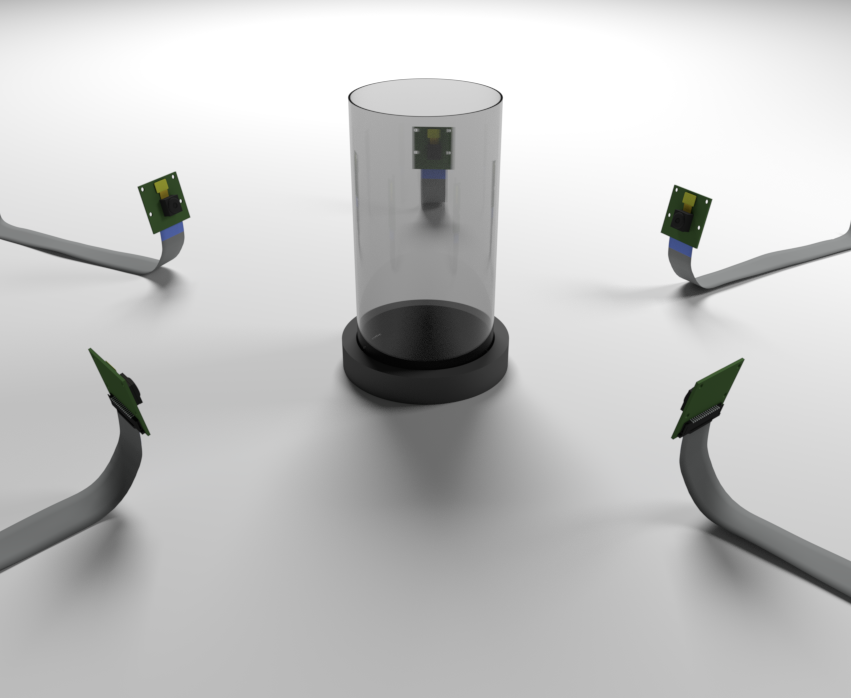
\includegraphics[width=0.95\textwidth]{images/renderCylinder.png}
		\caption{bisheriger Ansatz}
		\label{fig:oldSetup}
	\end{subfigure}%
	\begin{subfigure}{.5\textwidth}
		\centering
		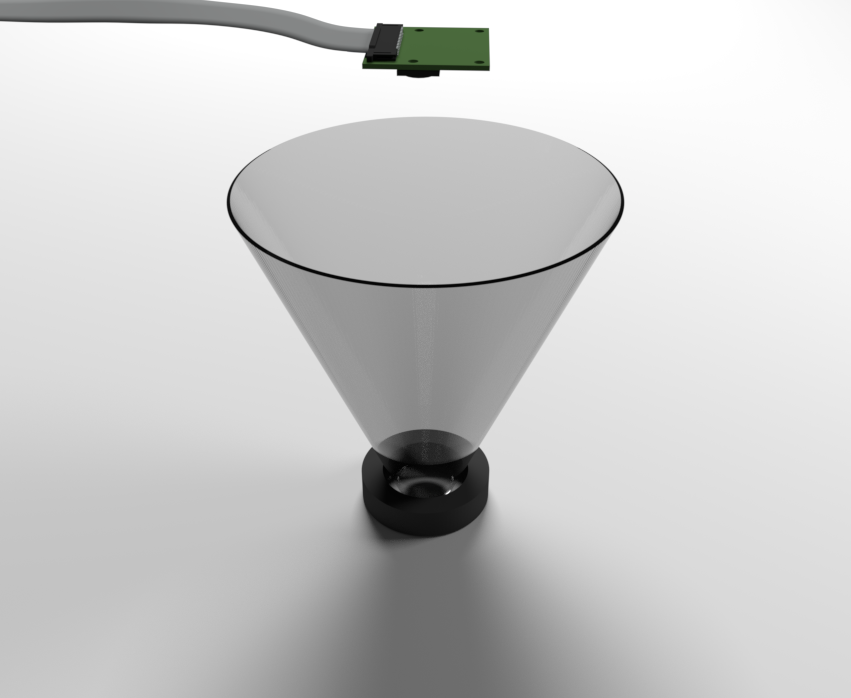
\includegraphics[width=0.95\textwidth]{images/renderCone.png}
		\caption{neuer Ansatz}
		\label{fig:newSetup}
	\end{subfigure}
	\caption{beide Ansätze im Vergleich}
	\label{fig:renderedSetup}
\end{figure}

\cleardoubleoddemptypage
%!TEX root = bachelor.tex
\chapter{Theoretische Grundlagen}
\label{ch:theory}

%In diesem Kapitel werden einige grundlegende Begriffe und Definitionen eingeführt, die in der folgenden Arbeit benötigt werden. 
%
%Wir benutzen ein linkshändiges Koordinatensystem.
%\todo{theorie einleitung schreiben}


\section{Kegel}
\label{s:cone}

\begin{definition}[Kegel]
	Ein Kegel ist ein geometrischer Körper, der durch eine beliebige Grundfläche, sowie einen Punkt definiert wird.
	Ein Kegel mit Kreis als Grundfläche wird als Kreiskegel bezeichnet. Liegt die Kegelspitze auf einer Geraden durch die Normale der Grundebene, bezeichnen wir den Kegel als gerade.
\end{definition}

In der weiteren Arbeit betrachten wir nur gerade Kreiskegel. Ein Kegel mit Spitze $T(0,0,0)$, Radius $R$ und Höhe $H$ kann parametrisch beschrieben werden als:
\begin{equation} \label{eq:paramCone}
\begin{aligned}
x &= \frac{u}{H} R~cos \theta \\
y &= u \\
z &= \frac{u}{H} R~sin \theta
\end{aligned}
\end{equation} %
mit $u\in [0, H]$ und $\theta \in [0, 2\pi)$ 

$S$ bezeichne hierbei die Seitenhöhe und sei definiert durch das rechtwinklige Dreieck mit den Seitenlängen $H,R$ und $S$ (siehe Abbildung \ref{fig:cone}). Es gilt $S = \sqrt{H^2 + R^2}$.

\begin{figure}[!htb]
	\centering
	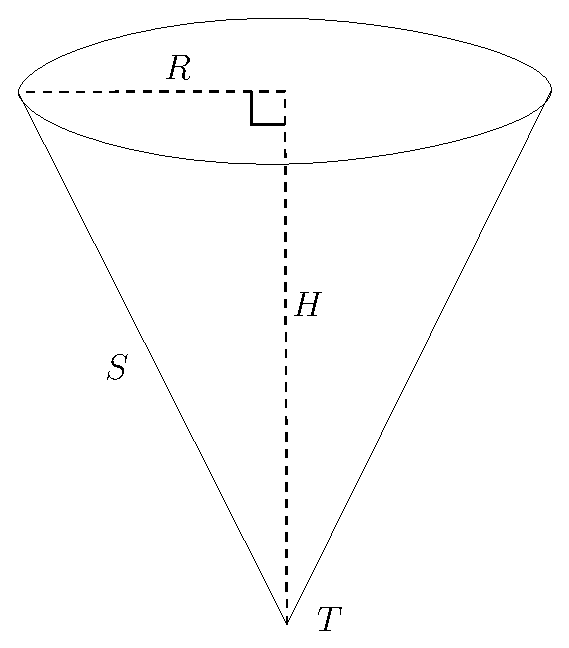
\includegraphics[scale=.5]{images/fullCone.eps}
	\caption{Gerader Kreiskegel}
	\label{fig:cone}
\end{figure}




\begin{definition}[Kegelstumpf und Ergänzungskegel]
	Ein Kegelstumpf entsteht als Schnitt eines geraden Kreiskegels mit einer zur Grundfläche parallelen Ebene (siehe Abbildung \ref{fig:coneWithFrustum}). Der Kegel, der definiert ist durch die Schnittfläche und die Spitze des ursprünglichen Kegels bezeichnen wir als Ergänzungskegel. Die Differenz des eigentlichen Kegels und des Ergänzungskegels bezeichnen wir als Kegelstumpf. 
	
	\noindent $H, R, S$ sind dabei weiterhin die Höhe, Radius und Seitenhöhe des gesamten Kegels. Hinzu kommen $h,r,s$ als Höhe, Radius und Seitenhöhe des Ergänzungskegels. Die Höhe, sowie die Seitenhöhe des Kegelstumpfs werden durch die Differenzen $\Delta S = S - s,~ \Delta H = H-h$ charakterisiert (siehe Abbildung \ref{fig:coneFrustum}).
\end{definition}

\begin{figure}[!htb]
	\centering
	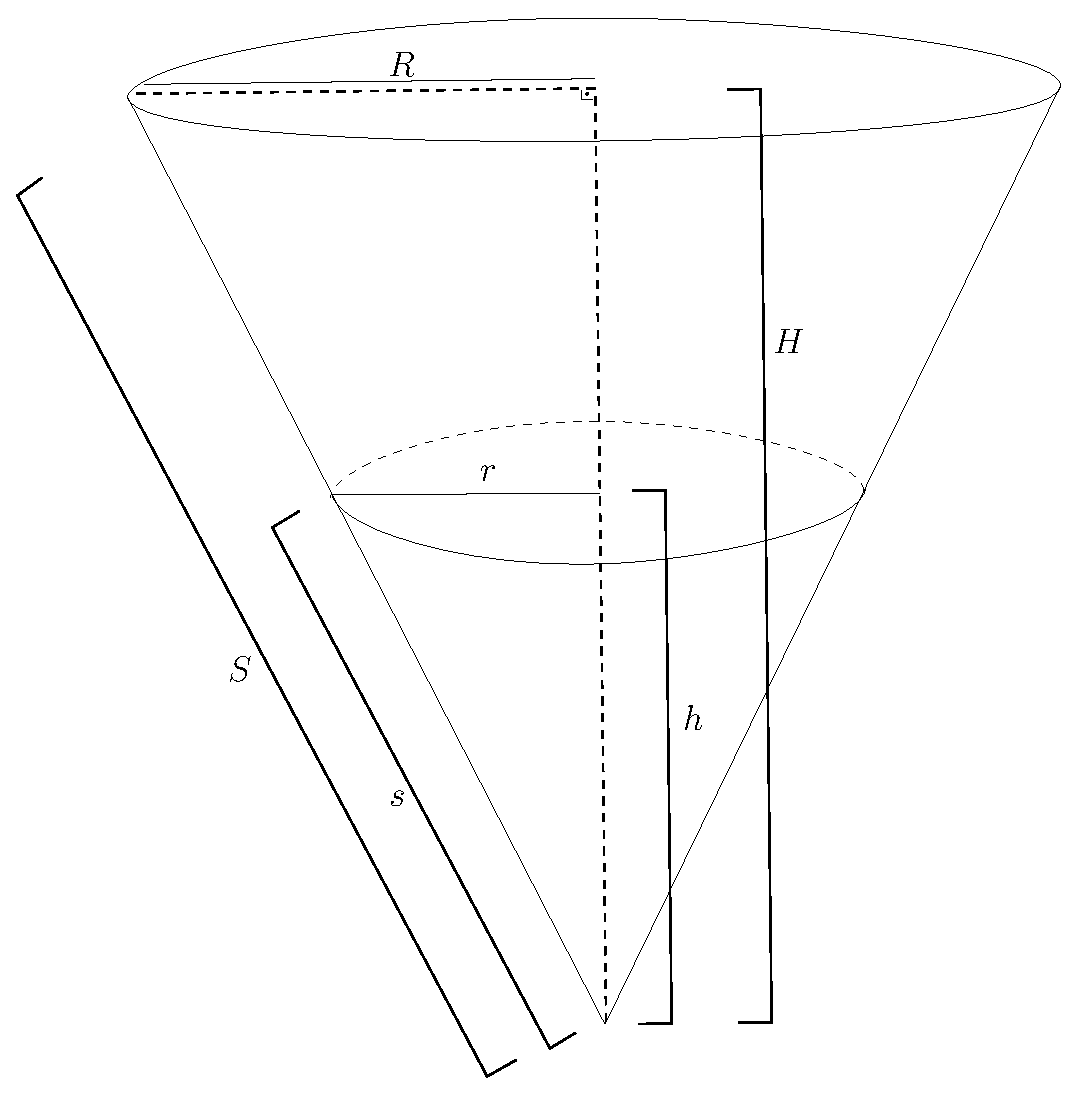
\includegraphics[scale=.5]{images/fullCone3.eps}
	\caption{Kegelstumpf und Ergänzungskegel}
	\label{fig:coneWithFrustum}
\end{figure}

\begin{figure}[!htb]
	\centering
	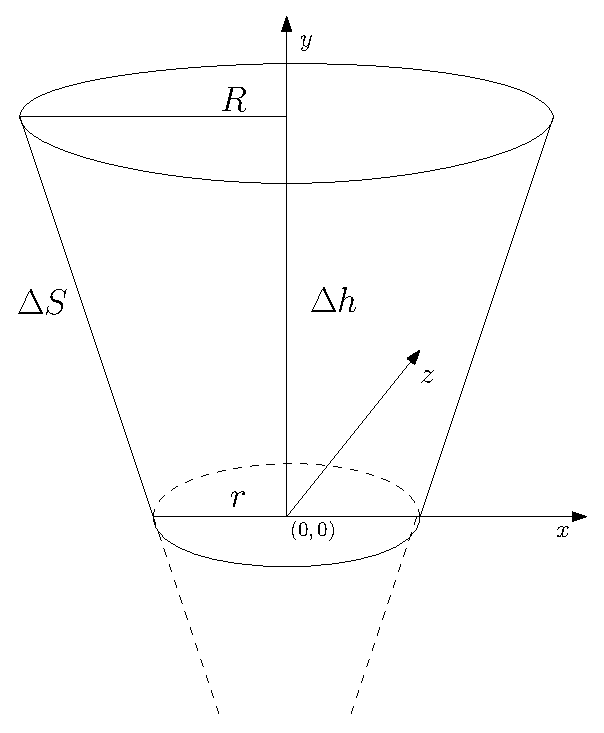
\includegraphics[scale=.7]{images/coneFrustum.eps}
	\caption{Kegelstumpf}
	\label{fig:coneFrustum}
\end{figure}

Wir definieren einen Kegelstumpf mit Zentrum $(0,0,0)$ des kleineren Kreises mit Radius $r$ durch folgende Parametrisierung: 
\begin{equation} \label{eq:paramFrustum}
\begin{aligned}
x &= (r + \frac{u}{\Delta H} (R - r))~cos \theta \\
y &= u \\
z &= (r + \frac{u}{\Delta H} (R - r))~sin \theta
\end{aligned}
\end{equation}
mit $u\in [0, \Delta H]$ und $\theta \in [0, 2\pi)$. Die parametrische Form eines Kegelstumpfs ist somit ein Verallgemeinerung der Parametrisierung von klassischen Kegeln (siehe Gleichung \ref{eq:paramCone}), wobei beim klassischen Kegel $r = 0$ gilt. Wie in Abbildung \ref{fig:coneFrustum} zu sehen, wollen wir bei Höhe $u=0$ einen Radius von $r$ erreichen. Wir führen also eine Skalierung des Intervalls $[0, R]$ auf das Intervall $[r, R]$ durch. Dies erreichen wir durch den Term $(r + \frac{u}{\Delta H} (R - r))$. \bigskip



Die Mantefläche des Kegelstumpfes aus Abbildung \ref{fig:coneLateral} kann dann in Polarkoordinaten parametrisch beschrieben werden als
\begin{equation} \label{eq:paramLateral}
\begin{aligned}
x &= -(s + \frac{u}{\Delta H}(S-s)) ~sin \phi \\
y &= (s + \frac{u}{\Delta H} (S-s)) ~cos \phi
\end{aligned}
\end{equation}
mit  $u\in [0, \Delta H]$ und $\phi \in [0, \alpha] \subseteq [0, 2\pi]$. 

\begin{figure}[!htb]
	\centering
	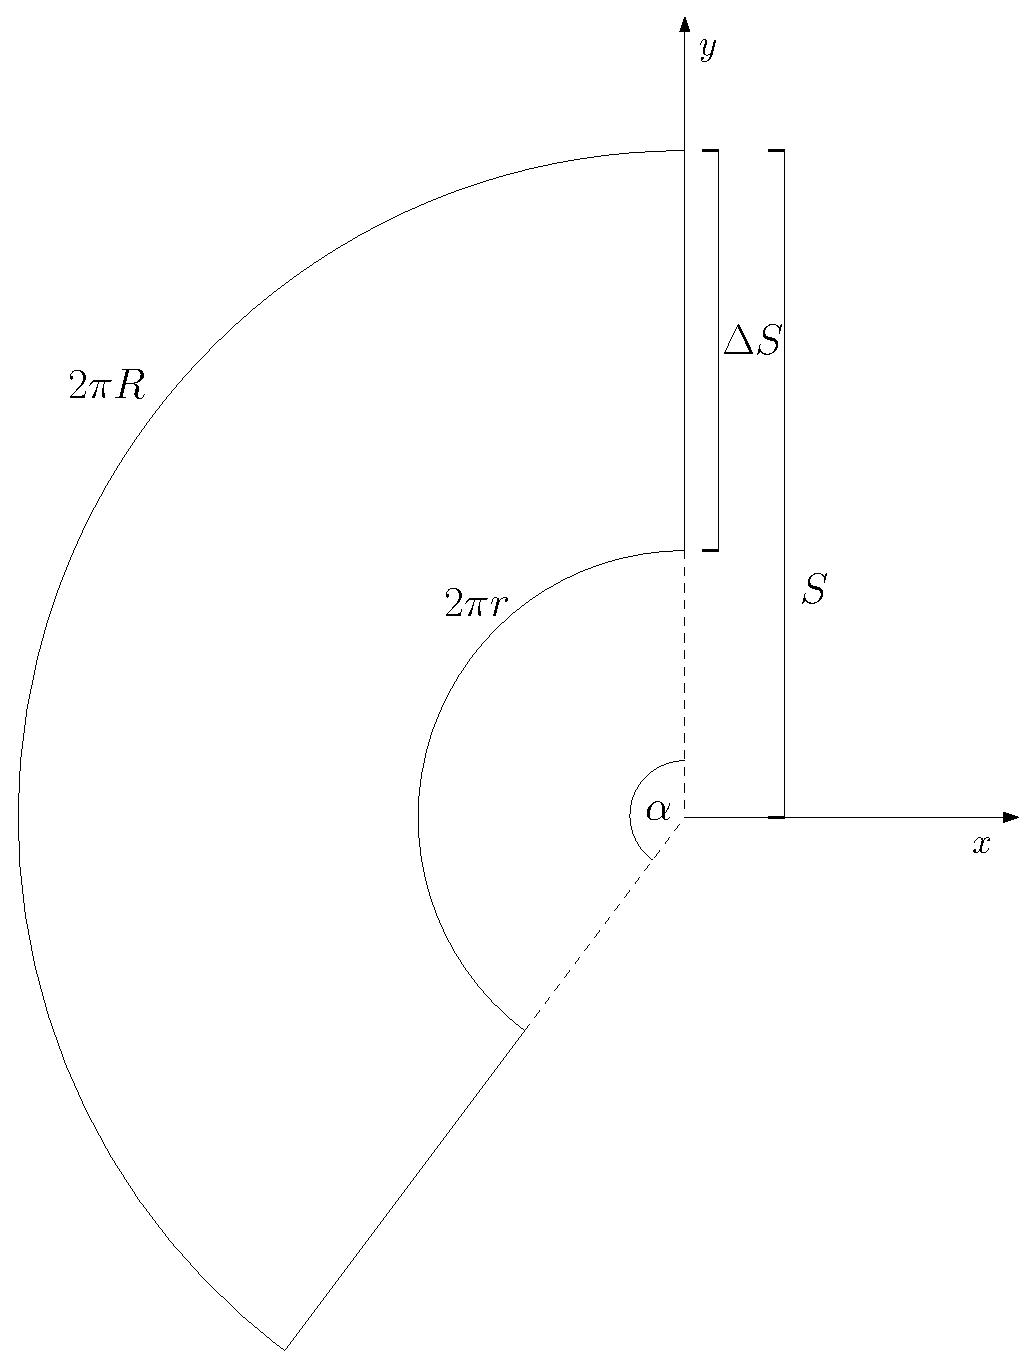
\includegraphics[scale=.4]{images/coneLateral.eps}
	\caption{Kegelmantelfläche}
	\label{fig:coneLateral}
\end{figure}

Die Mantelfläche ergibt sich durch Entrollen des Kegelstumpfs. Da der Umfang des Kreises mit Radius $R$, $2\pi R$ beträgt, muss, wie in Abbildung \ref{fig:coneLateral} zu sehen, der äußere Kreisbogen die Bogenlänge $2\pi R$ haben. Analog beträgt die Bogenlänge des inneren Kreisbogens $2\pi r$. Für den Winkel $\alpha$ muss demnach gelten $\alpha S = 2\pi R$, also  $\alpha = 2\pi\frac{R}{S}$. Da sich die Seitenhöhe, wie in Abbildung \ref{fig:mapToLateralS} zu sehen, linear zur Höhe des Kegelstumpfs verhält, kann die Seitenhöhe durch die Höhe ausgedrückt werden mit $(s + \frac{u}{\Delta H}(S-s))$. Bei Höhe $u = 0$ ergibt sich somit, wie erwartet die Seitenhöhe $s$, bei Höhe $u = \Delta H$ die Seitenhöhe $S$.


\begin{figure}[!htb]
	\centering
	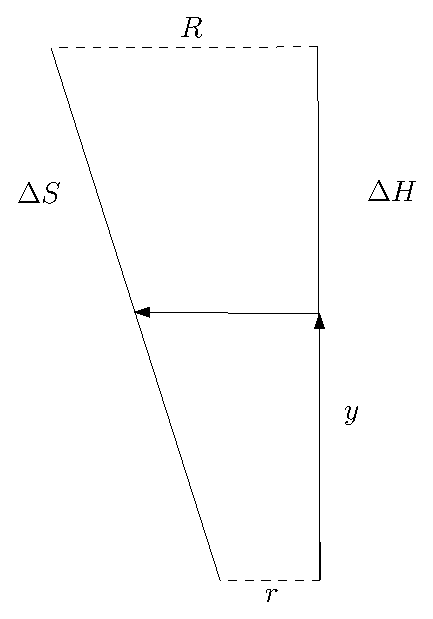
\includegraphics[scale=.7]{images/mapToLateralS.eps}
	\caption{Abbildung der Kegelstumpfhöhe auf die Seitenhöhe}
	\label{fig:mapToLateralS}
\end{figure}

\bigskip

Ein Punkt auf der Oberfläche des Kegelstumpfs kann eindeutig einem Punkt auf der Mantelfläche (und umgekehrt) zugeordnet werden. Dazu konstruieren wir folgende Abbildung und ihr Inverses:

Sei dazu ein Punkt $C(x,y,z)$ auf der Oberfläche des Kegelstumpfs gegeben. Gegeben durch die parametrischen Gleichung \ref{eq:paramFrustum}, hat $C$ die Form
\[
C(x,y,z) = (r + \frac{u}{\Delta H} (R - r))~cos \theta, u, (r + \frac{u}{\Delta H} (R - r))~sin \theta
\]  für ein $u\in [0, \Delta H]$ und $\theta \in [0, 2\pi)$. 

Aus der $y$-Koordinate lässt sich direkt die Höhe $u$ ablesen und somit analog zur Gleichung \ref{eq:paramLateral} die zugehörige Seitenhöhe, also der Radius der Polarkoordinaten in der parametrischen Gleichung  der Mantelfläche bestimmen.  Wir definieren uns hierfür eine Hilfsfunktion 
\begin{equation} \label{eq:help1}
	\Sigma(y) := s + \frac{y}{\Delta H} (S-s)
\end{equation}


Da $R, r, \Delta H$  und nun auch die Höhe bekannt sind, können wir den Winkel $\theta$ im Kegelstumpf ausrechnen. Anschließend muss dieser noch mit  $\frac{R}{S}$ multipliziert werden um ihn auf $[0, \alpha]$ zu skalieren (siehe Gleichung \ref{eq:paramLateral}).  Wir wollen in der Gleichung \ref{eq:paramFrustum} nach $\cos\phi$, beziehungsweise nach $\sin\phi$ umstellen und anschließend nach $\phi$ auflösen. Wir teilen also zunächst beide Gleichungen durch $r + \frac{y}{\Delta h} (R - r)$. Zu beachten ist nun, dass wir nicht die Umkehrfunktionen $\text{acos}$ oder $\text{asin}$ benutzen können, da $\sin$ und $\cos$ in einer Periode $[0, 2\pi)$ nicht injektiv sind. Die Wertebereiche der Umkehrfunktionen sind also eingeschränkt und wir erhalten somit im Allgemeinen nicht den korrekten Winkel in $[0, 2\pi)$. Das gleiche Problem zeigt sich bei $\tan\phi = \frac{\sin\phi}{\cos\phi}$ und der Umkehrfunktion $\atano$. Um dieses Problem zu beheben muss man eine Fallunterscheidung durchführen und wir definieren die Funktion $\atant$
\[
\atant(y,x) = 	\begin{cases}
					\atano \frac{y}{x} 					& \mbox{für } x > 0 \\ 
					\atano \frac{y}{x} + \frac{\pi}{2}	& \mbox{für } x < 0, y \geq 0 \\
					\atano \frac{y}{x} - \frac{\pi}{2}	& \mbox{für } x < 0, y < 0 \\
					\atano +\frac{\pi}{2}				& \mbox{für } x = 0, y > 0 \\
					\atano -\frac{\pi}{2}				& \mbox{für } x = 0, y < 0 \\
					0									& \mbox{für } x = 0, y = 0,
				\end{cases}
\]

die den Winkel $\phi$ im richtigen Quadranten,also in $[0, 2\pi)$ bestimmt.

Wir definieren wieder eine Hilfsfunktion
\begin{equation} \label{eq:help2}
\Phi(x,y,z) := \frac{R}{S} \atant\left(\frac{z}{r + \frac{y}{\Delta h} (R - r)}, \frac{x}{r + \frac{y}{\Delta H} (R - r)}\right).
\end{equation}

Mit den beiden Hilfsfunktionen \ref{eq:help1} und \ref{eq:help2}, sowie der Gleichung \ref{eq:paramLateral} ergibt sich insgesamt
\begin{equation}\label{eq:coneToLateral}
\begin{aligned}
\Psi \colon [r,R] \times [0, \Delta H] \times [r,R] &\to [s,S] \times [s,S]\\
\begin{pmatrix}
x \\ y \\ z
\end{pmatrix}  &\mapsto
\begin{pmatrix}
-\Sigma(y)\sin \Phi(x,y,z)\\
 \Sigma(y)\cos\Phi(x,y,z).
\end{pmatrix}
\end{aligned}
\end{equation}

Analog lässt die sich Umkehrabbildung konstruieren:

Sei ein Punkt $L(x,y)$ auf der Mantelfläche des Kegelstumpfs gegeben. Aus der parametrischen Form der Mantelfläche (siehe Gleichung \ref{eq:paramLateral}) ergibt sich

\[
L(x,y) = (-(s + \frac{u}{\Delta H}(S-s)) ~sin \phi, (s + \frac{u}{\Delta H} (S-s)) ~cos \phi)
\]

für ein passendes $u\in [0, \Delta H]$ und $\phi \in [0, \alpha] \subseteq  [0, 2\pi]$.

Da $L(x,y)$ in Polarkoordinaten gegeben ist, lässt sich der Radius durch $\sqrt{x^2+y^2}$ bestimmen. Wir können den Winkel $\phi$ mit inverser Skalierung also analog zu oben durch folgende Hilfsfunktion bestimmen:

\begin{equation}\label{eq:help3}
\Theta(x,y) := \frac{S}{R} \atant\left(-\frac{x}{\sqrt{x^2+y^2}}, \frac{z}{\sqrt{x^2+y^2}}\right)
\end{equation}

Die Höhe  im Kegel und somit der Radius lässt sich nun als Umkehrabbildung zu \ref{eq:help1} bestimmen:
\begin{equation}\label{eq:help4}
\mathrm{H}(x,y) := \frac{\left(\sqrt{x^2+y^2}\right) - s}{S - s}\Delta H
\end{equation}

Insgesamt ergibt sich:
\begin{equation}\label{eq:LateralToCone}
\begin{aligned}
\Psi^{-1} \colon  [s,S]\times[s,S] &\to [r,R] \times [0, \Delta H] \times [r,R]\\
\begin{pmatrix}
x \\ y
\end{pmatrix} &\mapsto
\begin{pmatrix}
\left( r + \frac{\mathrm{H}(x,y)}{\Delta H} (R - r)\right)\cos\left(\Theta(x,y) \right) \\
\mathrm{H}(x,y)\\
\left( r + \frac{\mathrm{H}(x,y)}{\Delta H} (R - r)\right)\sin\left(\Theta(x,y) \right)
\end{pmatrix}
\end{aligned}
\end{equation}


\section{Lineares Ausgleichsproblem}
\label{s:LSQ}
Gegeben seien $m$ Messdaten $(x_1,y_1),\dotsc,(x_m,y_m)$, sowie eine lineare Funktion $\varphi(x) = \sum_{i = 1}^{n}c_i\varphi_i(x)$ in $x$ mit $c_1,\dotsc,c_n\in\mathbb{R}$, Funktionen $\varphi_1,\dotsc,\varphi_n$, $n\leq m$ und $n,m\in\mathbb{N}$. 

Gesucht ist eine Lösung welche die mittlere Abweichung

\[
\Delta_2 = \min_{c_1,\dotsc,c_n\in\mathbb{R}} \left(\sum_{j=1}^{m}\left(y_j - \varphi(x_j)\right)^2\right) = \min_{c_1,\dotsc,c_n\in\mathbb{R}} \left(\sum_{j=1}^{m}\left(\sum_{i=1}^{n}y_j-\left(c_i\varphi_i(x_j)\right)\right)^2\right)
\]

minimiert \cite{Stoer2007}.

Diese Problem wird als lineares Ausgleichsproblem oder als Methode der kleinsten Quadrate bezeichnet und lässt sich wie folgt formulieren:

\[
\min_{c\in\mathbb{R}^n} ||y - Ac||_2,
\]

mit 
\[
\begin{aligned}
c &= (c_1,\dotsc,c_n)^T\in\mathbb{R}^n \\
x &= (x_1,\dotsc,x_m)^T\in\mathbb{R}^m \\
y &= (y_1,\dotsc,y_m)^T\in\mathbb{R}^m \\
A &= (a_{ij})\in\mathbb{R}^{m\times n}\quad\text{mit}\quad a_{ij} = \varphi_i(x_j)
\end{aligned}
\]

Das Problem lässt sich auch mit Hilfe der äquivalenten sogenannten Normalengleichung
\begin{equation*}
	(A^TA)c = A^Ty
\end{equation*}

lösen, wobei mindestens eine Lösung existiert und bei mehreren Lösungen, die Lösung mit kleinster 2-Norm ausgewählt wird. 

Gilt darüber hinaus $\text{rang}\left(A\right) = n$ so ist $A^TA$ invertierbar und es gilt 

\begin{equation}\label{eq:normaleq}
c = \underbrace{(A^TA)^{-1}A^T}_{A^+}y.
\end{equation}

Dabei ist c die eindeutige Lösung mit kleinster 2-Norm. $A^+$ bezeichnet man auch als Pseudoinverse von $A$. Im Allgemeinen ist die Matrix $A^TA$ nicht invertierbar. Die Pseudoinverse kann somit nicht einfach mit $(A^TA)^{-1}A^T$ berechnet werden. Stattdessen lässt sie sich durch eine Singulärwertzerlegung (SVD) bestimmen \cite{Stoer2011}. Die Matrizen $A\in\mathbb{R}^{m\times n}$ und $A^+\in\mathbb{R}^{n\times m}$ können geschrieben werden als:

\[
\begin{aligned}
A &= U\Sigma V^T \\
A^+ &= V\Sigma^+U^T
\end{aligned}
\]

mit orthogonalen Matrizen $U\in\mathbb{R}^{m\times m}$ und $V\in\mathbb{R}^{n\times n}$ und einer Diagonalmatrix $\Sigma\in\mathbb{R}^{m\times n}$ mit den absteigend sortierten Singulärwerten auf der Diagonale (aufgefüllt mit Nullen), sowie $\Sigma^+\in\mathbb{R}^{n\times m}$ mit den jeweiligen reziproken Singulärwerten.


Die Lösung des Ausgleichsproblems kann also mittels SVD angeben werden als:
\[
c = V\Sigma^+U^Ty
\]
Zu beachten ist, dass dieses Vorgehen auch bei Matrizen $A$ mit $\text{rang}\left(A\right) = n$ funktioniert, also wenn $A^TA$ invertierbar ist und darüberhinaus numerisch stabil implementiert werden kann \cite{Stoer2011}.



\section{Kamerakalibrierung}
\label{s:calib}

%\begin{definition}
%	Kamerakalibrierung ist ein Verfahren, bei dem die interne Kamerageometrie und optischen Eigenschaften (intrinische Parameter) 
%	und/oder die 3D-Position und Orientierung der Bildebene relativ zu einem Weltkoordinatensystem (extrinische Parameter) bestimmt werden \cite{Tsai1987}.
%\end{definition}
%\bigskip
Um die Parameter einer Kamera korrekt beschreiben zu können, ist ein Kameramodell notwendig. Das wohl bekannteste Kameramodell ist das Lochkamera-Modell. Die Lichtstrahlen der Szene gelangen dabei durch eine kleine Öffnung in die Kamera (siehe dazu Abbildung \ref{fig:pinhole}).
\begin{figure}[!htb]
	\centering
	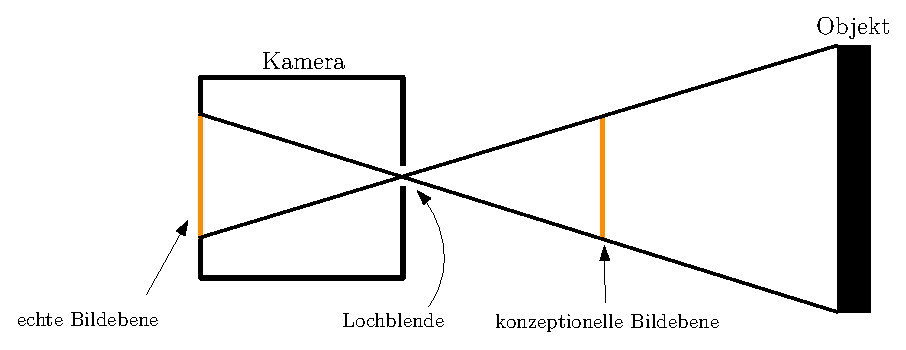
\includegraphics[scale=.8]{images/pinhole2.eps}
	\caption{Lochkameramodell}
	\label{fig:pinhole}
\end{figure}

Das Bild das an der Rückseite der Kamera entsteht ist dabei um 180° gedreht. Damit man diese Rotation nicht betrachten muss, kann man die Bildebene virtuell vor die Lochblende setzen. Da sich der Abstand zur Blende somit nicht ändert, ändern sich auch die optischen Eigenschaften nicht.

Kamerakalibrierung wird benötigt, um eine Beziehung zwischen Punkten im dreidimensionalen Weltkoordinatensystem und den Punkten auf der zweidimensionalen Bildebene herstellen zu können. Konkret suchen wir eine projektive Abbildung

\begin{equation}\label{eq:projectionMat}
	\begin{pmatrix}
	wu \\wv \\w 
	\end{pmatrix} = 
		\underbrace{\begin{pmatrix}
		a_{11} & a_{12} & a_{13} & a_{14} \\
		a_{21} & a_{22} & a_{23} & a_{24} \\
		a_{31} & a_{32} & a_{33} & a_{34} 
		\end{pmatrix}}_{=:A}	\begin{pmatrix}
		x \\y \\z \\ 1 
		\end{pmatrix},
\end{equation}


die einen Punkt $P=(x,y,z)$ in homogenen Koordinaten $\tilde P = (x,y,z,1)$ auf einen Punkt $\tilde C = (wu,wv, w)$ beziehungsweise nach der perspektivischen Division $C = (u,v)$ auf die Bildebene abbildet, wobei die $a_{ij}$ von den intrinsischen und extrinsischen Parametern der Kamera abhängen \cite{Heikkila1997}.

%Man kann leicht zeigen, dass für $A$ gilt
%\[
%A = \lambda \cdot
%\begin{pmatrix}
%1 & 0 & u_0\\
%0 & 1 & v_0\\
%0 & 0 & 1 
%\end{pmatrix}
%\begin{pmatrix}
%f & 0 & 0\\
%0 & f & 0\\
%0 & 0 & 1 
%\end{pmatrix} 
%\left(\begin{array}{ccc}
%R &  T\\
%0 & 1 
%\end{array}\right) = \lambda\underbrace{\begin{pmatrix}
%f & 0 & u_0\\
%0 & f & v_0\\
%0 & 0 & 1 
%\end{pmatrix}}_{=:V}
%\left(\begin{BMAT}(e)[1pt]{ccc|c}{ccc|c}
%& & & \\
%& \text{\large R}& & \text{\large T} \\
%& &  & \\
%0 & 0 & 0 & 1
%\end{BMAT}\right),
%\]
%
%wobei $\lambda$ ein beliebiger Skalierungsfaktor ist. $V$ beschreibt die intrinsischen und $R$ und $T$ die extrinsischen Parameter (siehe \cite{Heikkila1997}). $f$ ist hierbei die Brennweite; $(u_0, v_0)$ die Bildmitte.

%Zunächst wird also das Weltkoordinatensystem wie in Abbildung \ref{fig:extrinsic} mit einer Rotation und einer Translation in das Kamerakoordinatensystem überführt. Anschließend wird 
 
Man kann die Matrix $A$ mit gegebene Punktkorrespondenzen bestimmen. Wir benötigen dafür Punkte $(x_k,y_k, z_k), k = 1,\dotsc,m$ im Weltkoordinatensystem und die korrespondierenden Punkte $(u_k, v_k)$ auf der Bildebene.
Wir stellen zunächst das Gleichungssystems \ref{eq:projectionMat} nach $u$ und $v$ um:
 
 \begin{equation*}
 \begin{aligned}
 u_k &= \frac{a_{11} x_k +a_{12}y_k + a_{13}z_k + a_{14}}{a_{31} x_k +a_{32}y_k + a_{33}z_k + a_{34}} \\
 v_k &= \frac{a_{21} x_k +a_{22}y_k + a_{23}z_k + a_{24}}{a_{31} x_k +a_{32}y_k + a_{33}z_k + a_{34}}.
 \end{aligned}
 \end{equation*}
 
Wir wollen nun die $a_{ij}$ als Unbekannte betrachten und formulieren das Gleichungssystem noch einmal um zu:
 
 \setcounter{MaxMatrixCols}{20}
\begin{equation}\label{eq:DLT}
\underbrace{\begin{pmatrix}
x_1 & y_1 & z_1 & 1 & 0 & 0 & 0 & 0 & -u_1 x_1 & -u_1 y_1 & -u_1z_1 \\
0 & 0 & 0 & 0 & x_1 & y_1 & z_1 & 1 & -v_1x_1 & -v_1y_1 & -v_1z_1 \\
\vdots & \vdots & \vdots & \vdots & \vdots & \vdots & \vdots & \vdots & \vdots & \vdots & \vdots\\
x_m & y_m & z_m & 1 & 0 & 0 & 0 & 0 & -u_m x_m & -u_m y_m & -u_m z_m \\
0 & 0 & 0 & 0 & x_m & y_m & z_m & 1 & -v_mx_m & -v_my_m & -v_mz_m
\end{pmatrix}}_{=:M}
\begin{pmatrix}
a_{11} \\ a_{12} \\ a_{13} \\ a_{14} \\ a_{21} \\ a_{22} \\ a_{23} \\ a_{24} \\ a_{31} \\ a_{32} \\ a_{33}
\end{pmatrix} = 
\begin{pmatrix}
u_1 \\ v_1 \\ \vdots \\ u_m \\ v_m
\end{pmatrix},
\end{equation}

wobei $a_{34}$ auf eins skaliert wird. Dies ist erlaubt, da wir in homogenen Koordinaten rechnen und dies durch die perspektivischen Division kompensiert wird.  Es handelt sich hierbei für $m \geq 6$ um ein überbestimmtes lineares Gleichungssystem, was mittels der Methode der kleinsten Quadrate (siehe Kapitel \ref{s:LSQ}) und durch eine Singulärwertzerlegung gelöst werden kann. 
Diese Verfahren wird auch als \textit{Direct Linear Transformation} (DLT) bezeichnet.
 
Das beschriebene Verfahren vernachlässigt dabei Linsenverzerrungen. Solche Verzerrungen entstehen entweder als Produktionsfehler günstiger Linsen, oder werden durch spezielle Linsen, wie bei Weitwinkelkameras, begünstigt.  Verzerrungen können in der Regel nicht linear modelliert werden. Der Ansatz über DLT funktioniert hier dementsprechend nicht. 

Es wird grundsätzlich zwischen zwei Typen von Verzerrungen unterschieden: radiale Verzerrung und tangentiale Verzerrung. Radialen Verzerrung entsteht durch eine Skalierung des Abstand eines Bildpunktes zum Fokus. Wird der Abstand vergrößert spricht man von einer tonnenförmigen Verzerrung (siehe Abbildung \ref{fig:barrel}), wird er verkleinert von einer kissenförmigen Verzerrung (siehe Abbildung \ref{fig:cushion}).
Radiale Verzerrung kann wie folgt modelliert werden:

\[
\begin{aligned}
\hat{x}^{(r)} &= x\left[1 + k_1\left(x^2 + y^2\right) + k_2\left(x^2 + y^2\right)^2 + \dotsc\right] \\
\hat{y}^{(r)} &= y\left[1 + k_1\left(x^2 + y^2\right) + k_2\left(x^2 + y^2\right)^2 + \dotsc\right],
\end{aligned}
\]

wobei $(x,y)$ ein verzerrter Bildpunkt, $(\hat{x}^{(r)}, \hat{y}^{(r)})$ der entzerrte Punkt und $k_1$ und $k_2$ die Koeffizienten der radialen Verzerrung sind \cite{Zhang2002}.

Tangentiale Verzerrung ist auf eine fehlerhafte Fertigung zurückzuführen und entsteht beispielsweise wenn sich eine Linse nicht parallel zur Bildebene befindet. 
Sie kann modelliert werden durch:
\[
\begin{aligned}
\hat{x}^{(t)} &= \left[2p_1xy + p_2\left((x^2 + y^2) + 2x^2\right)\right] \\
\hat{y}^{(t)} &= \left[p_1\left((x^2 + y^2) + 2y^2\right) + 2p_2xy\right],
\end{aligned}
\]

wobei $(x,y)$ wieder ein verzerrter Bildpunkt, $(\hat{x}^{(t)}, \hat{y}^{(t)})$ der entzerrte Punkt und$p_1$ und $p_2$ die Koeffizienten der tangentialen Verzerrung sind \cite{Heikkila1997}.

\begin{figure}[!htb]
	\centering
	\begin{subfigure}{.33\textwidth}
		\centering
		
\includegraphics[width=0.9\textwidth]{images/undistorted.png}
		\caption{keine Linsenverrung}
		\label{fig:undist}
	\end{subfigure}%
	\begin{subfigure}{.33\textwidth}
		\centering
		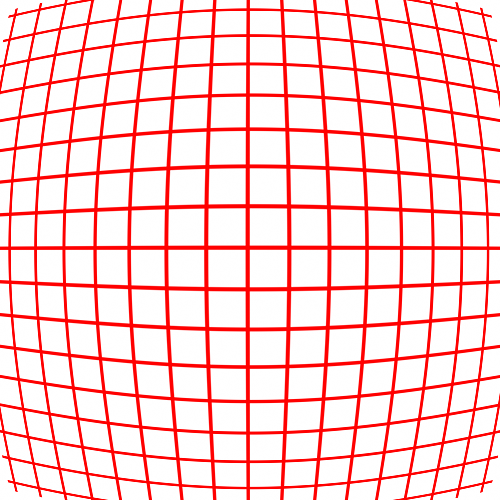
\includegraphics[width=0.9\textwidth]{images/barrelDistortion.png}
		\caption{tonnenförmige Verzerrung}
		\label{fig:barrel}
	\end{subfigure}%
	\begin{subfigure}{.33\textwidth}
		\centering
		
\includegraphics[width=0.9\textwidth]{images/cushionDistortion.png}
		\caption{kissenförmige Verzerrung}
		\label{fig:cushion}
	\end{subfigure}
	\caption{Linsenverzerrungen}
	\label{fig:distortion}
\end{figure}



\section{Blob-Detektor}
\label{s:blob}
\begin{definition}[Blob]\label{def:blob}
	Ein Blob ist eine glatte zusammenhängende Region in einem Bild, die sich farblich von ihrer Umgebung abhebt \cite{Lindeberg1993}.
\end{definition}

Ein Blob-Detektor ist also ein Verfahren zum Detektieren solcher Blobs. Die gefunden Blobs können anschließend nach verschiedenen Kriterien, wie beispielsweise Größe, Farbe, Konvexität oder Rundheit gefiltert werden. 

%\section{Canny}
%\label{s:canny}
%Der Canny-Algorithmus \cite{Canny1986} ist ein Verfahren zur Kantendetektion. Im Gegensatz zu anderen Verfahren wie Sobel, oder Prewitt, versucht Canny die Fehlerrate der Kantendetektion minimal zu halten. 
%Darüber hinaus markiert Canny die Kanten möglichst exakt, minimiert also die Distanz eines markierten Punktes zum eigentlich Zentrum der Kante. 
%Zuletzt gewährleistet Canny außerdem die Eindeutigkeit einer Kante. Das bedeutet, dass eine Kante nicht mehrmals markiert wird.

\section{Hough-Transformation}
\label{s:hough}
Hough-Transformation ist ein Verfahren zur Detektion von beliebigen parametrisierbaren Konturen. In dieser Arbeit werden Hough-Transforamtionen benutzt um Geraden zu detektieren. 

Eine beliebige zweidimensionale Gerade kann in Polarkoordinaten folgendermaßen implizit ausgedrückt werden:

\begin{equation}\label{eq:HoughLines}
x\cos\phi + y\sin\phi = d,
\end{equation}

wobei $\phi \in [0,2\pi)$ der Winkel der Geraden mit der $x$-Achse und $d \geq 0$ der Radius, also der euklidische Abstand der Geraden zum Ursprung des Koordinatensystems ist.

Eine Gerade wird somit als ein Punkt $(d,\phi)$ in den Parameterraum (auch Hough-Raum) abgebildet. 

Um eine Gerade eindeutig zu definieren benötigt man, wie auch bei der klassischen Defintionen $y = mx + b$, zwei Punkte. Nimmt man nur einen, so lässt sich jedoch die Auswahl von $\phi$ und $d$ einschränken. Hat man beispielsweise einen Punkt $(x_k,y_k)$ gegeben so lässt sich die Gleichung \ref{eq:HoughLines} nach $d$ umstellen und man erhält eine sinusförmige Funktion in Abhängigkeit von $\phi$. 

Um nun beliebige Geraden detektieren zu können, werden $\phi$ und $d$ zunächst passend diskretisiert:
\[
	\begin{aligned}
		\phi_i &= \phi_{min} + \frac{i}{n} \cdot (\phi_{max} - \phi_{min}) \quad&\forall &i\in [0,n]\\
		d_j &= d_{min} + \frac{j}{m} \cdot  (d_{max} - d_{min}) &\forall &j\in [0,m]
	\end{aligned}
\]



Es wird nun ein Akkumulator $\mathcal{H}(\phi, d)$ für alle $\phi_i$ und $d_j$ auf null gesetzt.
Als Nächstes wird ein Kantentbild mittels Canny \cite{Canny1986} erzeugt. Die Kantenpixel werden mit $(x_k,y_k)$ für $k = 0,\dotsc,l$ identifiziert. Das eigentliche Verfahren funktioniert nach folgendem Schema:

\begin{algorithm}
	\caption{Hough-Transformation}\label{euclid}
	\begin{algorithmic}[1]
		\For{$k = 0 ~\textbf{to}~ l$} \Comment{für alle Kantenpunkte}
		\For{$i = 0 ~\textbf{to}~ n$} \Comment{für alle diskreten Winkel $\phi_i$}
		\State $d \gets x\cos\phi_i + y\sin\phi_i$
		\State $d_i \gets \textbf{round}(d)$ \Comment{runde $d$ zum nächsten diskreten $d_i$}
		\State  $\mathcal{H}(\phi_i, d_i) \gets \mathcal{H}(\phi_i, d_i) + 1$
		\EndFor
		\EndFor
	\end{algorithmic}
\end{algorithm}

Die Werte im Akkumulator werden oft auch als Votes bezeichnet. Am Ende des Verfahrens such man im Akkumulator nach Häufungspunkten. Jeder Häufungspunkt steht dort für einen Geradenkandidaten.


%Zu einen gegebenen Pixel wir nun für alle diskreten Winkel $\phi_i$ ein Wert für $d$ ausgerechnet und auf den nächsten diskreten Wert $d_j$ gerundet. Anschließend wird im Akkumulator  $\mathcal{H}$ der Wert an der Stelle $(\phi_i, d_j)$ erhöht. Für jeden Kantenpunkt werden sinusförmige diskrete Funktionen in den Hough-Raum abgebildet. Die Werte im Akkumulator werden oft auch als Votes bezeichnet.
%Am Ende des Verfahrens such man im Akkumulator nach Häufungspunkten. Jeder Häufungspunkt steht dort für einen Geradenkandidaten.


\section{RANSAC}
\label{s:ransac}
\textit{Random Sample Consensus} (RANSAC) \cite{Fischler1981} ist ein nicht-deterministisches robustes Verfahren zur Parameterschätzung eines Modells bei einer, möglicherweise durch starke Ausreißer, gestörten Messreihe. 
Im Gegensatz zu Verfahren, wie der Methode der kleinsten Quadrate, die versuchen eine optimale Lösung für alle Messdaten zu bestimmen, nutzt RANSAC nur eine Teilmenge der Messreihe. 

Wir wählen aus der Menge der Messdaten wiederholt zufällig die minimale Anzahl Messdaten aus, die nötig sind um das Modell eindeutig zu beschreiben und prüfen dann, wie gut das geschätzte Modell die restlichen Messdaten beschreibt. 
Die Güte des Modells wird im Allgemeinen durch ein Distanzmaß, wie zum Beispiel der euklidische Abstand, berechnet. 
Hat ein Messdatum eine vorher definierte Maximaldistanz zum geschätzten Modell nicht überschritten, wird es ins sogenannte Consensus Set des Modells aufgenommen. 
Das Modell mit dem größten Consensus Set wird schließlich ausgewählt. 

Die Anzahl der Iterationen, die mindestens notwendig sind, um mit einer Wahrscheinlichkeit von $p \in [0,1)$, bei einem relativen Ausreißeranteil von $\epsilon \in[0,1)$ und einer Anzahl von $k$ Daten, um das Modell eindeutig zu beschreiben, mindestens einmal eine ausreißerfreie Teilmenge der Messreihe zu erhalten, lässt sich berechnen mit \cite{Fischler1981}:

\begin{equation}
n_{min} = \frac{\log{\left(1-p\right)}}{\log{\left(1-\left(1-\epsilon\right)^k\right)}}
\end{equation}


\section{Ellipsen}
\label{s:ellipse}
\subsection{Definition}
\label{s:ellipseGeneral}

\begin{definition}[Ellipse]
	Eine Ellipse wird beschrieben durch diejenigen Punkte, dessen Summe der Abstände zu zwei gegebenen Punkten $f_1$ und $f_2$ (Brennpunkte) konstant sind. Der Mittelpunkt der Verbindungslinie der beiden Brennpunkt wird als Zentrum der Ellipse bezeichnet (siehe Abbildung \ref{fig:ellipseDef}). 
	Als Hauptachse $a$ bezeichnen wir die Verbindungslinie von Mittelpunkt durch einen der Brennpunkte bis zum Scheitelpunkt ($V_1$ beziehungsweise $V_3$) der Ellipse. Die zu ihr rechtwinklige Verbindungslinie durch den Mittelpunkt bis zu einem der anderen Scheitelpunkte ($V_2$ beziehungsweise $V_4$) nennen wir Nebenachse $b$.
\end{definition}

\begin{figure}[!htb]
	\centering
	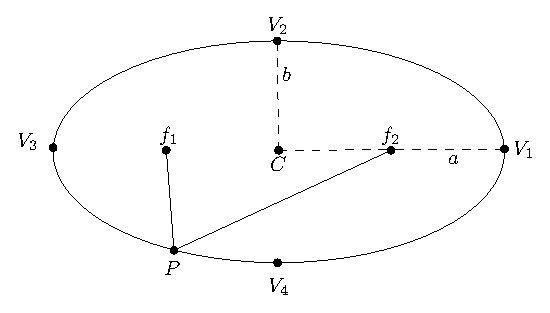
\includegraphics[scale=.9]{images/ellipse_focalDef.eps}
	\caption{Ellipse mit Brennpunkten $f_1, f_2$, Zentrum $C$, Hauptachse $a$, Nebenachse $b$ und Scheitelpunkten $V_1/V_3$ und $V_2/V_4$}
	\label{fig:ellipseDef}
\end{figure}

In ihrer einfachsten Form liegt die Ellipse im Zentrum des Koordinatensystems und ihre Haupt- und Nebenachse $a$ und $b$ sind achsenausgerichtet. Das heißt ihre Hauptachse liegt auf der $x$-Achse und ihre Nebenachse auf der $y$-Achse. Sie kann dann in der impliziten Form

\begin{equation} \label{eq:ellipseNoRotNoTrans}
\frac{x^2}{a^2} + \frac{y^2}{b^2} = 1
\end{equation} 

beschrieben werden.

\begin{figure}[!htb]
	\centering
	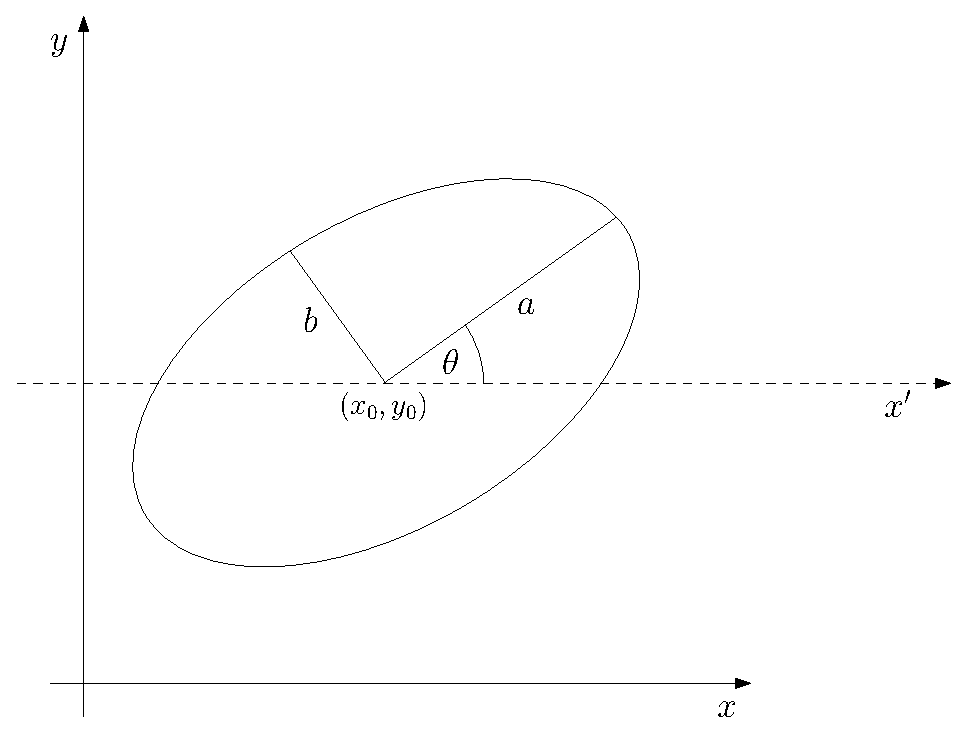
\includegraphics[scale=.7]{images/ellipse.eps}
	\caption{Ellipse mit Zentrum $(x_0, y_0)$, Hauptachse $a$, Nebenachse $b$, sowie Drehwinkel $\theta$}
	\label{fig:ellipse}
\end{figure}

Befindet sich die Ellipse nicht im Ursprung so muss eine Verschiebung beziehungsweise bei einer Rotation ein Drehwinkel (siehe Abbildung \ref{fig:ellipse}) ergänzt werden. 

\begin{equation} \label{eq:ellipseNoRotTrans}
\frac{\left(x-x_0\right)^2}{a^2} + \frac{\left(y-y_0\right)^2}{b^2} = 1
\end{equation} 

\begin{equation} \label{eq:ellipseRotTrans}
\frac{((x - x_0)\cos\theta + (y - y_0)\sin\theta)^2}{a^2} + \frac{((x - x_0)\sin\theta - (y - y_0)\cos\theta)^2}{b^2} = 1
\end{equation} 

mit Ellipsenzentrum $(x_0,y_0)\in\mathbb{R}^2$, Hauptachsen $a,b\in\mathbb{R}^+$, sowie Drehwinkel $\theta \in [0,2\pi)$ oder parametrisiert

\begin{equation} \label{eq:ellipseRotTransParam}
\begin{pmatrix}x \\ y\end{pmatrix} = \begin{pmatrix}x_0 + a\cos\phi\cos\theta - b\sin\phi\sin\theta \\ 
y_0 + a\cos\phi\sin\theta + b\sin\phi\cos\theta\end{pmatrix}
\end{equation}
mit $\phi \in [0, 2\pi)$ und $x_0, y_0, a,b, \theta$ wie oben.

In ihrer allgemeinsten Form lässt sich eine Ellipse durch ein implizites Polynom zweiten Grades charakterisieren
\begin{equation} \label{eq:ellipseQuadratic}
ax^2 + by^2 + cxy + dx + ey + f = 0 \quad \text{mit}\quad c^2-4ab < 0
\end{equation} 
mit $a,b,c,d,e,f \in \mathbb{R}$. Eine Ellipse lässt sich also durch sechs Punkte eindeutig beschrieben (fünf, wenn man $f$ auf eins skaliert).


Die beiden Formen \ref{eq:ellipseRotTrans} und \ref{eq:ellipseQuadratic} sind äquivalent, falls die Ellipse nicht degeneriert ist (ohne Beweis) \cite{Lawrence1972}. Die Umformung von \ref{eq:ellipseRotTrans} nach \ref{eq:ellipseQuadratic} ist mit Hilfe einer Hauptachsentransformation möglich. 
Da wir diese später brauchen, wird sie hier einmal exemplarisch vorgeführt. 

Zunächst einmal fällt auf, dass der gemischte Term $cxy$ genau dann null ist, wenn die Ellipse nicht rotiert wurde. Im ersten Schritt versuchen wir also die Rotation der Ellipse rückgängig zu machen, um den Rotationswinkel bestimmen zu können.

Die Gleichung \ref{eq:ellipseQuadratic} kann umgeformt werden zu:
\begin{equation*}
\begin{aligned}
\underbrace{\begin{pmatrix}x & y\end{pmatrix}}_{=:u^T}\underbrace{\begin{pmatrix}a & \frac{c}{2} \\ \frac{c}{2} & b\end{pmatrix}}_{=: M}\underbrace{\begin{pmatrix}x \\ y\end{pmatrix}}_{=u} +\begin{pmatrix}d & e\end{pmatrix}\underbrace{\begin{pmatrix}x \\ y\end{pmatrix}}_{=u}+ f = 0 \\
\Leftrightarrow u^TMu +\begin{pmatrix}d & e\end{pmatrix}u + f = 0 \\
\end{aligned}
\end{equation*} 
Der gemischte Term wird alleine durch $M = \begin{pmatrix}a & \frac{c}{2} \\ \frac{c}{2} & b\end{pmatrix}$ bestimmt. Die Matrix $M$ ist invertierbar, denn
\[
\det M = ab - \dfrac{c^2}{4}
\] ist nur dann gleich null, wenn $c^2 - 4ab = 0$, was ein Widerspruch zur Annahme in \ref{eq:ellipseQuadratic} ist. $M$ hat somit eine von null verschiedene Determinante und somit vollen Rang, hat also zwei von null verschiedene Eigenwerte \cite[S. 199]{Bosch2006}. Insbesondere gibt es also zwei Eigenvektoren von $M$, die zueinander orthogonal sind \cite[S. 198]{Bosch2006}.

Da die Matrix $M$ außerdem symmetrisch ist, ist sie orthogonal diagonalisierbar \cite[S. 278]{Bosch2006}.

Es gilt $M = S^TDS$, wobei $S\in\mathbb{R}^{2\times2}$ eine orthogonale Matrix mit den normierten Eigenvektoren als Zeilen und $D = \text{diag}(\lambda_1, \lambda_2)\in\mathbb{R}^{2\times2}$ eine Diagonalmatrix mit den beiden Eigenwerten von $M$ auf der Diagonalen ist. Ohne Beschränkung der Allgemeinheit gelte $\lambda_1 <= \lambda_2$, andernfalls vertausche die Eigenvektoren in $S$. 

Sei nun $v := Su$.
So gilt:

\begin{equation} \label{eq:PCARot}
\begin{aligned}
&u^T(S^TDS)u +\begin{pmatrix}d & e\end{pmatrix}\underbrace{(S^TS)}_{=\ind}u + f = 0 \\
\Leftrightarrow\quad &(Su)^TD(Su) +\begin{pmatrix}d & e\end{pmatrix}S^T(Su) + f = 0 \\
\Leftrightarrow\quad &v^{T}Dv +\begin{pmatrix}d & e\end{pmatrix}S^Tv + f = 0 \\
\Leftrightarrow\quad &\lambda_1v_1^2 + \lambda_2v_2^2 +\begin{pmatrix}d & e\end{pmatrix}S^Tv + f = 0 
\end{aligned}
\end{equation}

mit $v = (v_1,v_2)^T$. Man sieht, dass der gemischte Teil somit eliminiert wurde. Durch Anwenden der Transformation $S$ wurde $u$ also in das Koordinatensystem, in dem die Ellipse achsenausgerichtet ist,  transformiert.

Eine Rotationsmatrix mit Rotationswinkel $\theta$ ist definiert durch: 
\begin{equation}
\begin{aligned}
R = \begin{pmatrix}\cos\theta & -\sin\theta \\ \sin\theta & \cos\theta\end{pmatrix}
\end{aligned}
\end{equation}

Es gilt offenbar $S = R$ für ein geeignetes $\theta$, da die Eigenvektoren normiert und orthogonal zueinander sind. $\theta$ kann also einfach ausgerechnet werden, denn es gilt:

\begin{equation*}
\theta = \atant(\sin\theta, \cos\theta) = \atant(S_{2,1}, S_{1,1})
\end{equation*}

Formt man nun Gleichung \ref{eq:PCARot} weiter um, ergibt sich:

\begin{equation}\label{eq:ellipseCenter}
\begin{aligned}
&\lambda_1v_1^2 + \lambda_2v_2^2 + \underbrace{\begin{pmatrix}d & e\end{pmatrix}S^T}_{=:(d', e')}v + f = 0 \\
\Leftrightarrow\quad &\lambda_1v_1^2 + \lambda_2v_2^2 + d'v_1 + e'v_2 + f = 0 \\
\Leftrightarrow\quad &(\lambda_1v_1^2 + d'v_1)+ (\lambda_2v_2^2 + e'v_2) + f = 0\\
\Leftrightarrow\quad &(\lambda_1v_1^2 + d'v_1) + (\frac{d'^2}{4\lambda_1} - \frac{d'^2}{4\lambda_1}) + (\lambda_2v_2^2 + e'v_2) + (\frac{e'^2}{4\lambda_2} - \frac{e'^2}{4\lambda_2}) + f = 0 \\
\Leftrightarrow\quad &\left[\lambda_1\left(v_1^2 + \frac{2d'}{2\lambda_1}v_1 + \frac{d'^2}{4\lambda_1^2}\right) - \frac{d'^2}{4\lambda_1}\right] +\left[\lambda_2\left(v_2^2 + \frac{2e'}{2\lambda_2}v_2 + \frac{e'^2}{4\lambda_2^2}\right) - \frac{e'^2}{4\lambda_2}\right] + f = 0 \\
\Leftrightarrow\quad &\lambda_1(v_1 + \underbrace{\frac{d'}{2\lambda_1}v_1}_{ = -x'_0})^2 +\lambda_2(v_2 + \underbrace{\frac{e'}{2\lambda_2}v_2}_{ = -y'_0})^2 - \underbrace{(\frac{d'^2}{4\lambda_1} + \frac{e'^2}{4\lambda_2} - f)}_{=:\sigma} = 0,
\end{aligned}
\end{equation}

da $\lambda_1, \lambda_2 \neq 0$. 

Vergleichen wir diese Gleichung mit Gleichung \ref{eq:ellipseNoRotTrans}, so können wir das Zentrum der transformierten Ellipse $(x'_0, y'_0)$ aus Gleichung \ref{eq:ellipseCenter} einfach ablesen. Um das Zentrum der eigentlichen Ellipse zu bestimmen, müssen wir mit der inversen Rotation $S^T$ multiplizieren:
\[
(x_0, y_0)^T = S^T(x'_0, y'_0)^T
\]

Die Gleichung \ref{eq:ellipseCenter} lässt sich anschließend weiter vereinfachen: 


\begin{equation} \label{eq:PCAKoeff}
\begin{aligned}
&\lambda_1(v_1 -x'_0)^2 +\lambda_2(v_2 -y'_0)^2 = \sigma \\
\Leftrightarrow\quad & \frac{\lambda_1}{\sigma}(v_1 -x'_0)^2 +\frac{\lambda_2}{\sigma}(v_2 -y'_0)^2  =1
\end{aligned}
\end{equation}

wobei $\sigma \neq 0$, wenn die Ellipse nicht zum Punkt entartet ist (folgt aus dem Determinantenkriterium \cite{Lawrence1972}). Vergleichen wir nun die beiden Gleichungen \ref{eq:PCAKoeff}, sowie \ref{eq:ellipseNoRotTrans}, so können folgende Beziehung herleiten: 

\begin{equation}
\begin{aligned}
&\frac{\lambda_1}{\sigma} = \frac{1}{a^2} &\text{und}\quad &\frac{\lambda_2}{\sigma} = \frac{1}{b^2}\\
\Leftrightarrow\quad & \sqrt{\frac{\sigma}{\lambda_1}}  = a  &\text{und}\quad & \sqrt{\frac{\sigma}{\lambda_2}}  = b
\end{aligned}
\end{equation}

Wir dürfen hierbei die Wurzel ziehen, da $\frac{\sigma}{\lambda_i} > 0$ für nicht entartete reele\footnote{Man kann Ellipsen auch mit imaginären Achsen definieren \cite{Lawrence1972}.}  Ellipsen (folgt aus dem Determinantenkriterium \cite{Lawrence1972}). Da die Transformation in das Koordinatensystem der Ellipse nur Rotationen enthielt,  bleiben die Längen der Hauptachsen erhalten. Es gilt wie erwartet $a \geq b$, da $\lambda_1 \leq \lambda_2$. 


\subsection{Abstand: Punkt zu Ellipse}
\label{sc:distPointEllipse}
Das hier beschriebene Verfahren zur Bestimmung der kürzesten euklidischen Distanz eines Punktes zu einer Ellipse stammt aus der Arbeit von David Eberly \cite{Eberly2013}.
Wir betrachten nur Ellipsen im Ursprung, die achsenausgerichtet sind und darüber hinaus nur Punkte im ersten Quadranten. Ansonsten wir die Ellipse in den Ursprung verschoben und um ihren entgegengesetzten Drehwinkel rotiert. Da die Ellipse dann bezüglich der $x$- und $y$- Achse symmetrisch ist, kann der Punkt einfach durch Spiegelung in den richtigen Quadranten transformiert werden. Der Abstand ändert sich dadurch nicht. 

Wir bezeichnen von nun an $Q = (y_0, y_1)$ als eine Punkt, dessen Distanz zur Ellipse wir berechnen wollen und $E = (x_0, x_1)$ als denjenigen eindeutigen Punkt, welcher auf der Ellipse liegt und die kürzeste euklidische Distanz zum Punkt $Q$ hat. 

Aufgrund dieser Forderungen können wir ohne Beschränkung der Allgemeinheit folgende Aussagen treffen:
\begin{itemize}
	\item Die Ellipse kann stets durch die implizite Gleichung 
	\begin{equation}\label{eq:distEqParam} \frac{x_0^2}{a^2} + \frac{x_1^2}{b^2} = 1\end{equation}
	 mit $a \geq b \geq 0$ beziehungsweise
	in der parametrischen Form \[\mathcal{E}(\theta) = (a\cos\phi, b\sin\phi)  \tag*{$\phi \in [0, 2\pi)$}\] beschrieben werden.
	\item Es gilt $y_0,y_1,x_0, x_1 \geq 0$.
\end{itemize}

Für die quadrierte Distanz von einem beliebigen Punkt $Q$ zu einem Punkt $\mathcal{E}(\theta)$ auf der Ellipse gilt dann
\begin{equation}
	F(\theta) = \abs{\mathcal{E}(\theta) - Q}^2.
\end{equation}

Wir wollen $F$ minimieren und betrachten die Ableitung:
\begin{equation}\label{eq:perp}
F'(\theta) = 2\left(\mathcal{E}(\theta) - Q\right) \cdot \mathcal{E}'(\theta)
\end{equation}

$F'$ wird null, wenn $\left(\mathcal{E}(\theta) - Q\right)$ und $ \mathcal{E}'(\theta)$ zu einander orthogonal sind. Daraus folgt, dass der Vektor von $Q$ zu $E$ senkrecht zur Ellipse stehen muss (siehe Abbildung \ref{fig:ellipseDist}). 


\begin{figure}[!htb]
	\centering
	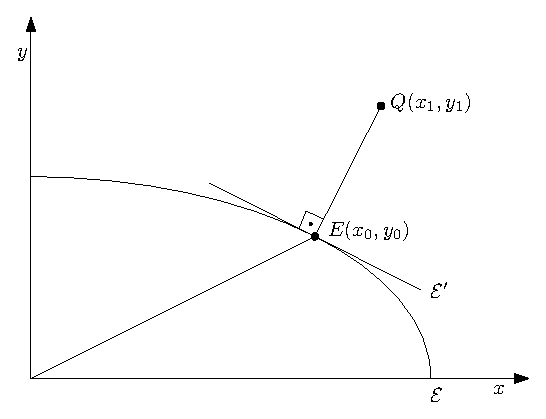
\includegraphics[scale=.9]{images/ellipseQuery.eps}
	\caption{Ellipsenausschnitt im ersten Quadranten mit Abfragepunkt $Q$ und eingezeichneter kürzester Distanz zum Ellipsenpunkt $E$. Die Ellipse wird beschrieben durch $\mathcal{E}$}
	\label{fig:ellipseDist}
\end{figure}

Betrachten wir die Funktion $G(z_0,z_1)$ basierend auf der impliziten Darstellung aus Gleichung \ref{eq:distEqParam}
\begin{equation} \label{eq:ellipseDistEq}
	G(z_0,z_1) = \frac{z_0^2}{a^2} + \frac{z_1^2}{b^2} - 1.
\end{equation}
Die Nullstellen von $G$ beschreiben somit die Ellipse. Sei nun solch eine Nullstelle gegeben als $(x_0,y_0)$. Der Gradient $\nabla G$ ist dann in $(x_0,x_1)$ ein Normalenvektor der Ellipse. Somit ist auch der halbe Gradient $\nabla G(x_0,x_1)/2$ ein Normalenvektor. Da aus Gleichung \ref{eq:perp}, die Orthogonalität von $\overrightarrow{QE}$ zur Ellipse folgt,  muss der Vektor  $\overrightarrow{QE}$ ein skalares Vielfaches des halben Gradienten sein. Es gilt somit:

\begin{equation}
	(y_0,y_1) - (x_0, x_1) = t\frac{\nabla G(x_0,x_1)}{2} = t\left(\frac{x_0}{a^2},\frac{x_1}{b^2}\right)
\end{equation}
für ein $t\in\mathbb{R}$.

Umgestellt nach $y_0$ und $y_1$, beziehungsweise nach $x_0$ und $x_1$ ergibt sich:

\begin{equation}\label{eq:ellipseDistY}
y_0 = x_0\left(1 + \frac{t}{a^2}\right), \quad y_1 = x_1\left(1 + \frac{t}{b^2}\right)
\end{equation}

\begin{equation}\label{eq:ellipseDistX}
x_0 = \frac{a^2y_0}{t+a^2},\quad x_1 = \frac{b^2y_1}{t+b^2}
\end{equation}


\bigskip
Man macht nun eine Fallunterscheidung:

\begin{enumerate}
	\item Der einfachste Fall ist, wenn sich der Punkt $Q$ auf der $y$-Achse (außer $(0,0)$) befindet, wenn also gilt $y_0 = 0, y_1 > 0$.
	Da die Hauptachse nach der $y$-Achse ausgerichtet ist und $a >= b$ gilt, ist der Punkt auf der Ellipse mit der kürzesten Distanz zu $Q$ offenbar $E = (0, b)$ und für die Distanz gilt $d = \abs{y_1 - b}$.
	\item Als nächstes betrachten wir ein $Q$ auf der $x$-Achse (einschließlich $(0,0)$), wenn also gilt  $y_0 \geq 0, y_1 = 0$. Es gilt also mit \ref{eq:ellipseDistY}
	\[
		y_0 = x_0\left(1 + \frac{t}{a^2}\right), \quad 0 = x_1\left(1 + \frac{t}{b^2}\right)
	\]
	
	Wenn $x_1 = 0$ gilt, muss $x_0 = a$ gelten, damit $E(x_0,x_1)$ auf der Ellipse ist. Es  gilt analog zum ersten Fall $E=(a,0)$ mit $d = \abs{y_0 - a}$ 
	
	Gilt $x_1 \neq 0$, so können wir in der zweiten Gleichung durch $x_1$ teilen und es folgt $t = -b^2$ und somit $y_0 = x_0\left(1 - \frac{b^2}{a^2}\right)$. Auf Grund der Krümmung der Ellipse gilt außerdem $x_0 < a$ und somit ergibt sich zusammen mit \ref{eq:ellipseDistX} die Ungleichung:
	\begin{equation*}
	\begin{aligned}
		&x_0 = \frac{a^2y_0}{a^2 - b^2} < a \\
		\Leftrightarrow\quad &y_0 < \frac{a^2 - b^2}{a} < a
	\end{aligned}
	\end{equation*}
		
	Für Punkte $Q(y_0,0)$ mit $y_0 \geq \frac{a^2 - b^2}{a}$, ist der kürzeste Punkt also wieder $E(a,0)$
	
	Für Punkte $Q(y_0,0)$ mit $y_0 < \frac{a^2 - b^2}{a}$, muss für $E(x_0,x_1)$ nach Umstellen der Ellipsengleichung \ref{eq:distEqParam}\quad$x_1 = b\cdot\sqrt{1-\left(\frac{x_0}{a}\right)}$ gelten. 
	Die Distanz beträgt dann:

	\[
		d^2 = (x_0 - y_0)^2 + x_1^2 = b^2\left(1 - \frac{y_0^2}{a^2 - b^2}\right)
	\]
	\item Der letzte Fall, den wir betrachten müssen, ist der allgemeinste Fall. Es gilt $y_0 > 0$, sowie $y_1 > 0$. Da wir uns nur im ersten Quadranten bewegen, gilt darüber hinaus $x_0, x_1 \geq 0$. Mit diesen Eigenschaften und \ref{eq:ellipseDistY} lässt sich folgende Einschränkung für $t$ herleiten:
\[
	\begin{aligned}
	& 0 < y_0 = x_0\left(1 + \frac{t}{a^2}\right)\\
	\Leftrightarrow\quad& -1\cdot a^2 < t.
	\end{aligned}
\]
	Analog ergibt sich mit $y_1\colon -b^2 < t$. Da $a\geq b$ gilt, reicht es, sich nur die zweite Ungleichung anzuschauen, da sie die erste impliziert. Setzt man nun \ref{eq:ellipseDistX} in \ref{eq:ellipseDistEq} ein, erhält man:
	
\[
	\begin{aligned}
		F(t) &= \left(\frac{a^2y_0}{a\left(t+a^2\right)}\right)^2 + \left(\frac{b^2y_1}{b\left(t+b^2\right)}\right)^2 - 1 \\
		&= \left(\frac{ay_0}{t+a^2}\right)^2 + \left(\frac{by_1}{t+b^2}\right)^2 - 1
	\end{aligned}
\]
	
	Durch Untersuchung der Ableitungen kann nun zeigen, dass diese Funktion auf dem gesamten Intervall $[-b^2,\infty)$ monoton fällt und links gekrümmt ist \cite{Eberly2013}. Darüber hinaus gilt:
	\[
	\lim\limits_{t \searrow -b^2}{F(t)}	= +\infty, \quad\lim\limits_{t \rightarrow \infty}{F(t)}	= -1.
	\]
	Da $F$ stetig ist, muss es also eine Nullstelle geben, die aufgrund des Monotonie- und Krümmungsverhaltens sogar eindeutig ist. Die Nullstelle lässt sich beispielsweise durch Intervallschachtelung oder Newton-Verfahren bestimmen. 
\end{enumerate}


\section{Analytical Deformable Templates}
\label{s:anaDef}
\textit{Analytical Deformable Templates} ist ein Verfahren zur Detektion von analytischen Kurven. 
Ein Template ist dabei definiert durch eine Menge von Parametern, die a priori Wissen über die erwartete Form ermöglichen. 
Als Beispiel sei eine  Ellipse genannt, die durch ihr Zentrum, ihren beiden Achsen und den Drehwinkel $(x_0,y_0,a,b,\phi)$ definiert ist.
Es wird dann eine Energiefunktion konstruiert, dessen Terme eine Anziehung des Templates an Hauptmerkmale (wie Kantenstärke, Kantenorientierung, Farbintensität, etc. ) des Bildes hervorrufen. 
Die Energiefunktion wird dabei durch numerische Verfahren, wie dem Gradientenverfahren, minimiert \cite{Yuille1992}. 








\cleardoubleoddemptypage
%!TEX root = bachelor.tex
\chapter{Methodik}
\label{ch:method}
In diesem Kapitel stellen wir zwei Verfahren zur Entzerrung von Kegeloberflächen vor.
Zunächst gehen wir auf das verwendete Kalibrierungsmuster ein, worauf hin die einzelnen Schritte der Entzerrung erläutert werden.

Die geometrischen Eigenschaften des Kegelstumpfs $(r, R, \Delta H)$ können gemessen und somit als bekannt angenommen werden.
Darüber hinaus nehmen wir an, dass sich das Zentrum des Deckkreises an der Position $(0,0,0)$, sowie das Zentrum des Grundkreises an der Position $(0,\Delta H, 0)$ im Weltkoordinatensystem befindet (siehe Abbildung \ref{fig:coneFrustum} in Kapitel \ref{s:cone}). Durch diese Einschränkung gehen jegliche absolute Größenverhältnisse verloren. Die Larven können jedoch weiterhin relativ zu einander verglichen werden.


\section{Kalibrierungsmuster}
\label{s:calibrationPattern}
\subsection{Aufbau des Kalibrierungsmusters}
Um eine Beziehung zwischen Bildpunkten und Kegelpunkten herstellen zu können, ist ein Kalibrierungsmuster notwendig.

Die Wahl des Kalibrierungsmusters spielt dabei eine entscheidende Rolle bei der Robustheit und Präzision der Entfaltung. Es muss gewährleistet sein, dass die charakteristischen Merkmale des Musters auch bei leichten Abweichungen der Kamera vom Lot und schlechteren Beleuchtungssituationen zuverlässig erkannt werden. Das Muster muss darüber hinaus so entworfen sein, dass beim Zusammenlegen im Kegel, dessen geometrische Eigenschaften nicht verfälscht, sondern realitätsgetreu wiedergeben werden.

Wir haben uns für ein Muster entscheiden, dass in äquidistanten Abständen $\Delta R$, beginnend mit dem Radius $r$ des Deckkreises (siehe Abbildung \ref{fig:coneFrustum}) Kreislinien und in gleichen Winkelabständen $\Delta \alpha$ auf der Seitenhöhe Liniensegmente besitzt. Das zusammengelegte Muster ist in Abbildung \ref{fig:calibrationPatternTop} skizziert, beziehungsweise das entfaltete in \ref{fig:calibrationPattern}. Die Anzahl der Kreislinien wird mit $n$ gekennzeichnet, die Anzahl sichtbarer Liniensegmente im Kegel mit $m$. Zu beachten ist, dass bedingt durch das Entfalten, in Abbildung \ref{fig:calibrationPattern}  ein Liniensegment doppelt zu sehen ist. Die schwarzen Kreise bezeichnen wir als Samples.

Dadurch dass die Geometrie des Kegels bekannt ist, kann jedem Sample ein Punkt auf dem Kegel im Weltkoordinatensystem zugeordnet werden. Da ein Kegel beliebig um die $y$-Achse rotiert werden kann, ist diese Zuordnung zunächst nicht eindeutig. Dazu nehmen wir an, dass das Liniensegment mit dem kleinsten Winkel zur $x$-Achse mit dem Kegelwinkel $\theta = 0$ korrespondiert (siehe Gleichung \ref{eq:paramFrustum} in Kapitel \ref{s:cone}).

\begin{figure}[!htb]
	\centering
	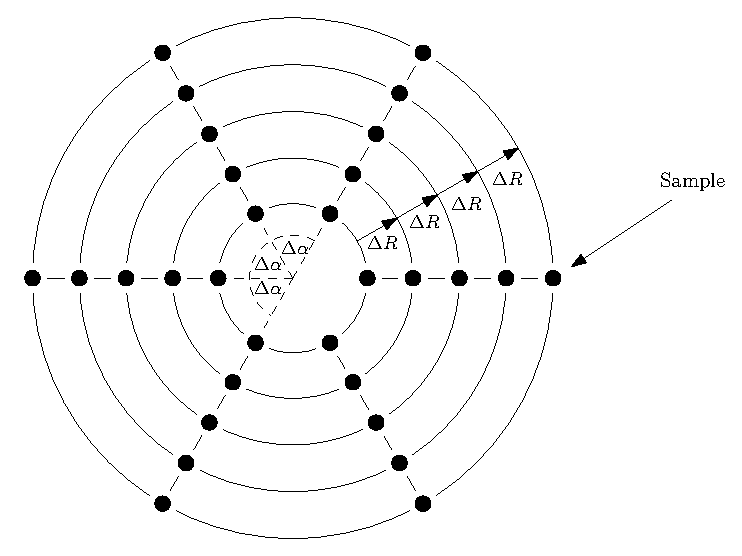
\includegraphics[scale=.8]{images/calibrationPatternTop.eps}
	\caption{Kalibrierungsmuster von oben mit $n = 5, m = 6$}
	\label{fig:calibrationPatternTop}
\end{figure}


\begin{figure}[!htb]
	\centering
	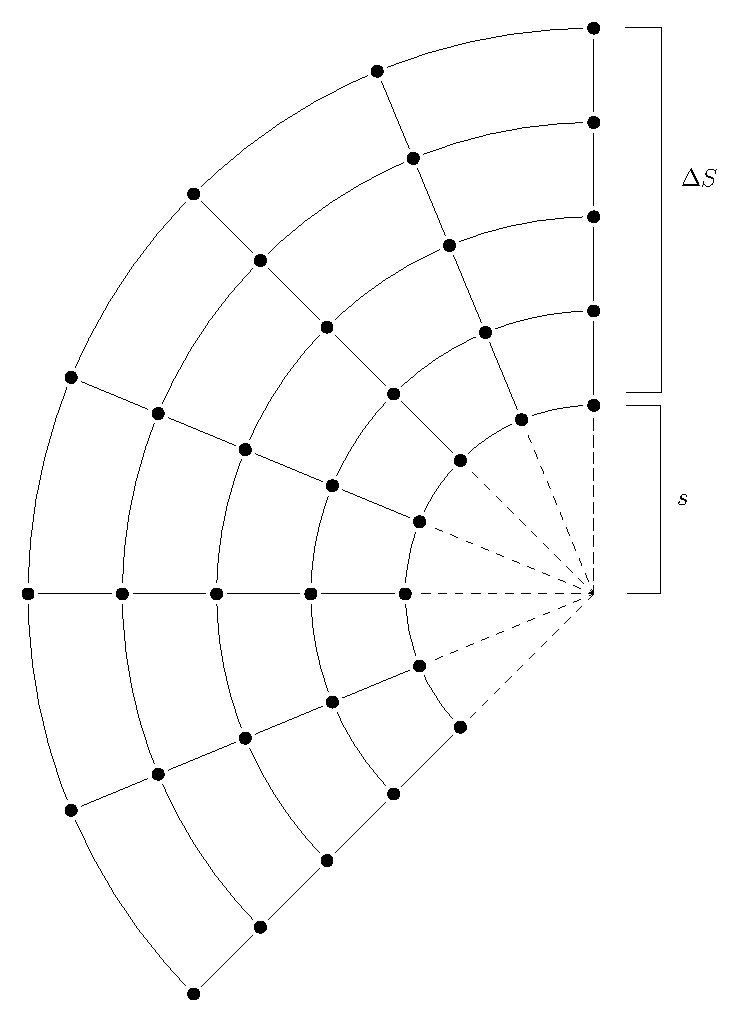
\includegraphics[scale=.7]{images/calibrationPattern2.eps}
	\caption{Kalibrierungsmuster entfaltet mit $n = 5, m = 6$}
	\label{fig:calibrationPattern}
\end{figure}

Zur Konstruktion des Musters benötigt man $\Delta S$ und $s$, die man aus der Geometrie des Kegels errechnen kann und außerdem den Öffnungswinkel, der gegeben ist als $\alpha = 2\pi\frac{R}{S}$ (siehe Gleichung \ref{eq:paramLateral} in Kapitel \ref{s:cone}).

\subsection{Anzahl der Samples}
Die Anzahl der Samples sollte groß genug sein, um möglichst viele geometrische Informationen des Kegels zu erhalten, aber klein genug, dass eine Detektion der Samples problemlos möglich ist. Insbesondere auf dem innersten Kreis, macht sich eine zu hohe Sampleanzahl negativ bemerkbar, da der Abstand der Samples zueinander sehr klein wird, was eine Detektion erschwert. Des Weiteren sollte noch ein möglichst großer Teil der Kreislinien zu sehen bleiben, da diese für die spätere Ellipsendetektion benötigt werden.


\section{Intrinsische Kamerakalibrierung}
\label{s:intrinsic}
Bedingt durch die Wahl einer Weitwinkelkamera, sind die Bilder von einer starken tonnenförmigen (nach außen gewölbte) Verzerrung geprägt, wie in Abbildung \ref{fig:calib} zu sehen. Diese muss herausgerechnet werden, da sonst Abstände im Bild nicht mehr der Realität entsprechen und dadurch die Präzision der Entfaltung stark abnimmt (siehe Kapitel \ref{ch:analysis}). Es wird also im ersten Schritt eine Kamerakalibrierung durchgeführt.


\begin{figure}[!htb]
	\centering
\begin{subfigure}{.5\textwidth}
	\centering
	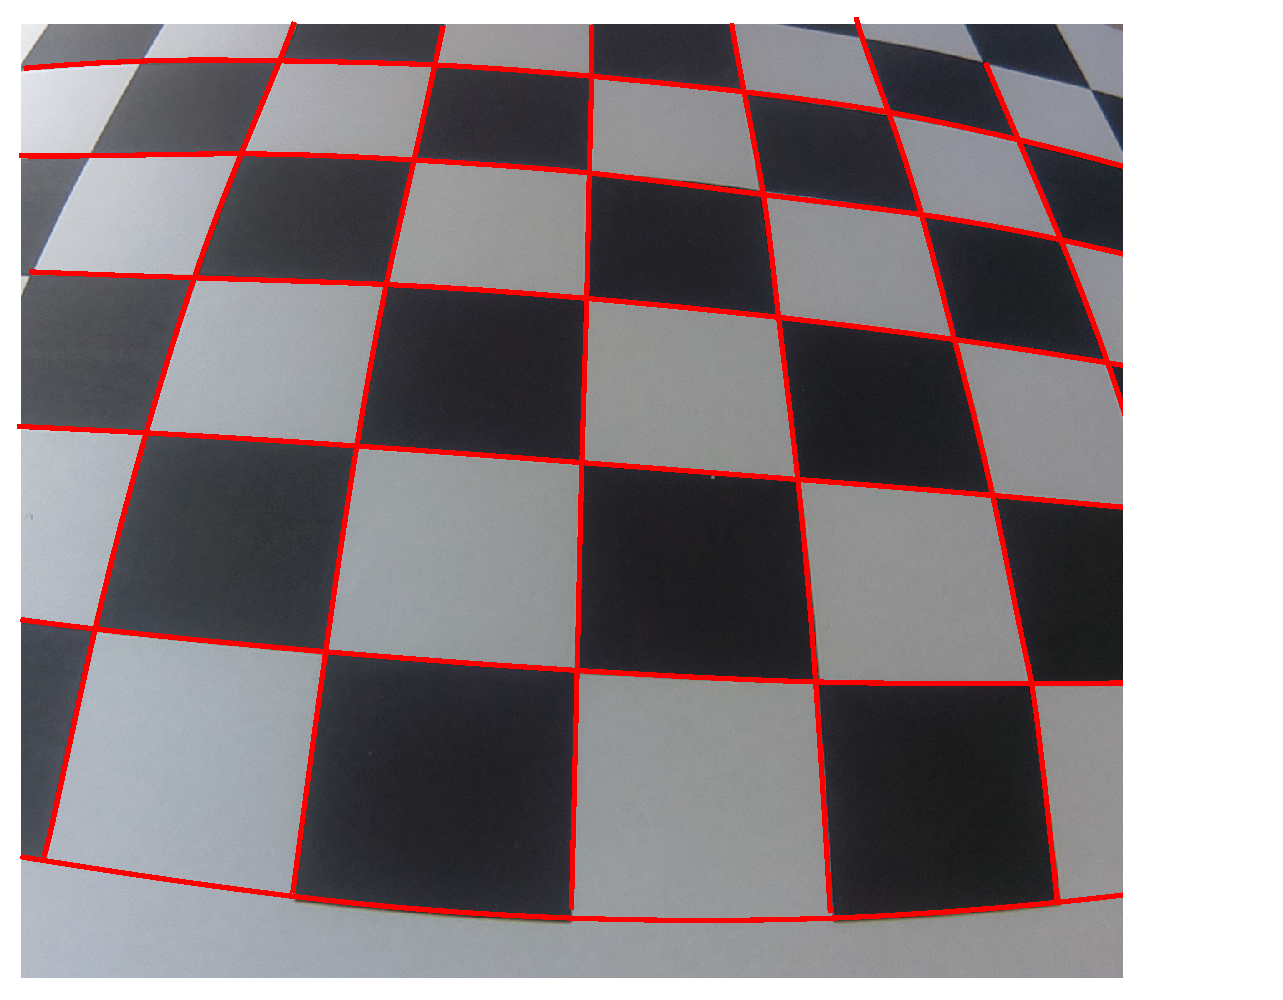
\includegraphics[scale=.35]{images/calibrationRaspi.eps}
	\caption{vor Kalibrierung}
	\label{fig:calibDist}
\end{subfigure}%
\begin{subfigure}{.5\textwidth}
	\centering
	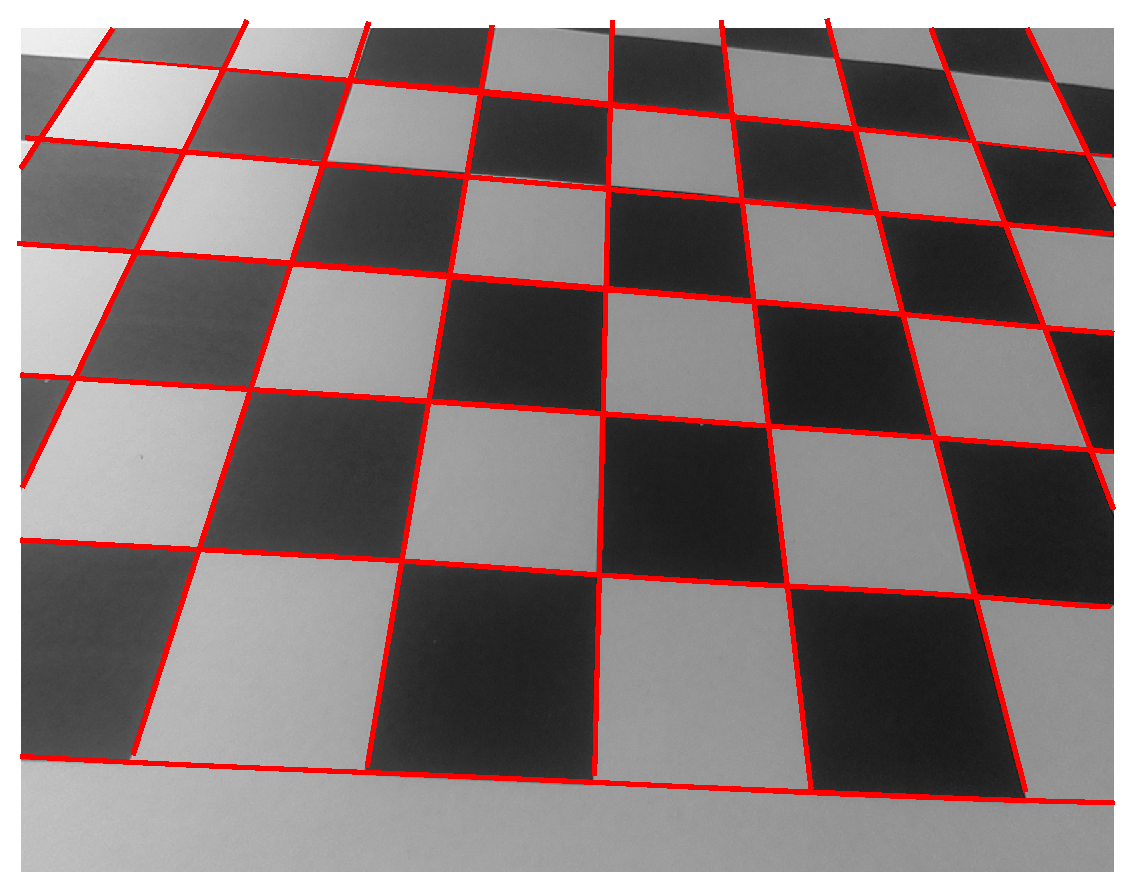
\includegraphics[scale=.4]{images/calibrationRaspi2.eps}
	\caption{nach Kalibrierung und Entzerrung}
	\label{fig:calibUndist}
\end{subfigure}
\caption{Kamerakalibrierung}
\label{fig:calib}
\end{figure}

\section{Detektion der charakteristischen Punkte}

Nach der Kamerakalibrierung und entsprechender Entzerrung werden die Bildkoordinaten der Samples bestimmt. Dazu wird ein Blob-Detektor (siehe Kapitel \ref{s:blob}) benutzt.
Um ein Sample korrekt detektieren zu können, muss sich der Punkt farblich stark von seiner Umgebung abheben (siehe Definition eines Blobs \ref{def:blob}). Das bedeutet, dass ein Sample freigestellt (helle homogene Umgebung) sein muss. Insbesondere dürfen die Kreislinien und Liniensegmente des Kalibrierungsmusters also nicht durchgezogen sein.

Nach der Detektion werden die Blobs nach folgenden Kriterien gefiltert:

\begin{itemize}
	\item \textbf{Fläche:} zu kleine Blobs werden verworfen
	\item \textbf{Rundheit:} zu unrude Blobs werden verworfen. Rundheit ist hier definiert als $circ = \frac{4\pi\cdot \textrm{Fläche}}{\left(\textrm{Umfang}\right)^2}\in[0,1]$, wobei ein Kreis mit $circ = 1$ maximal rund ist.
	\item  \textbf{Konvexität:} zu unkonvexe Blobs werden verworfen. Konvextität ist hier definiert \\als $conv = \frac{\textrm{Fläche Blob}}{\textrm{Fläche konvexe Hülle}}$
\end{itemize}

In Abbildung \ref{fig:blobDetect} ist beispielhaft links ein Grauwertbild und rechts die detektierten Blobs (rot) auf dem gleichen Bild nach der Kameraentzerrung zu sehen.


\begin{figure}[!htb]
	\centering
	\begin{subfigure}{.5\textwidth}
		\centering
		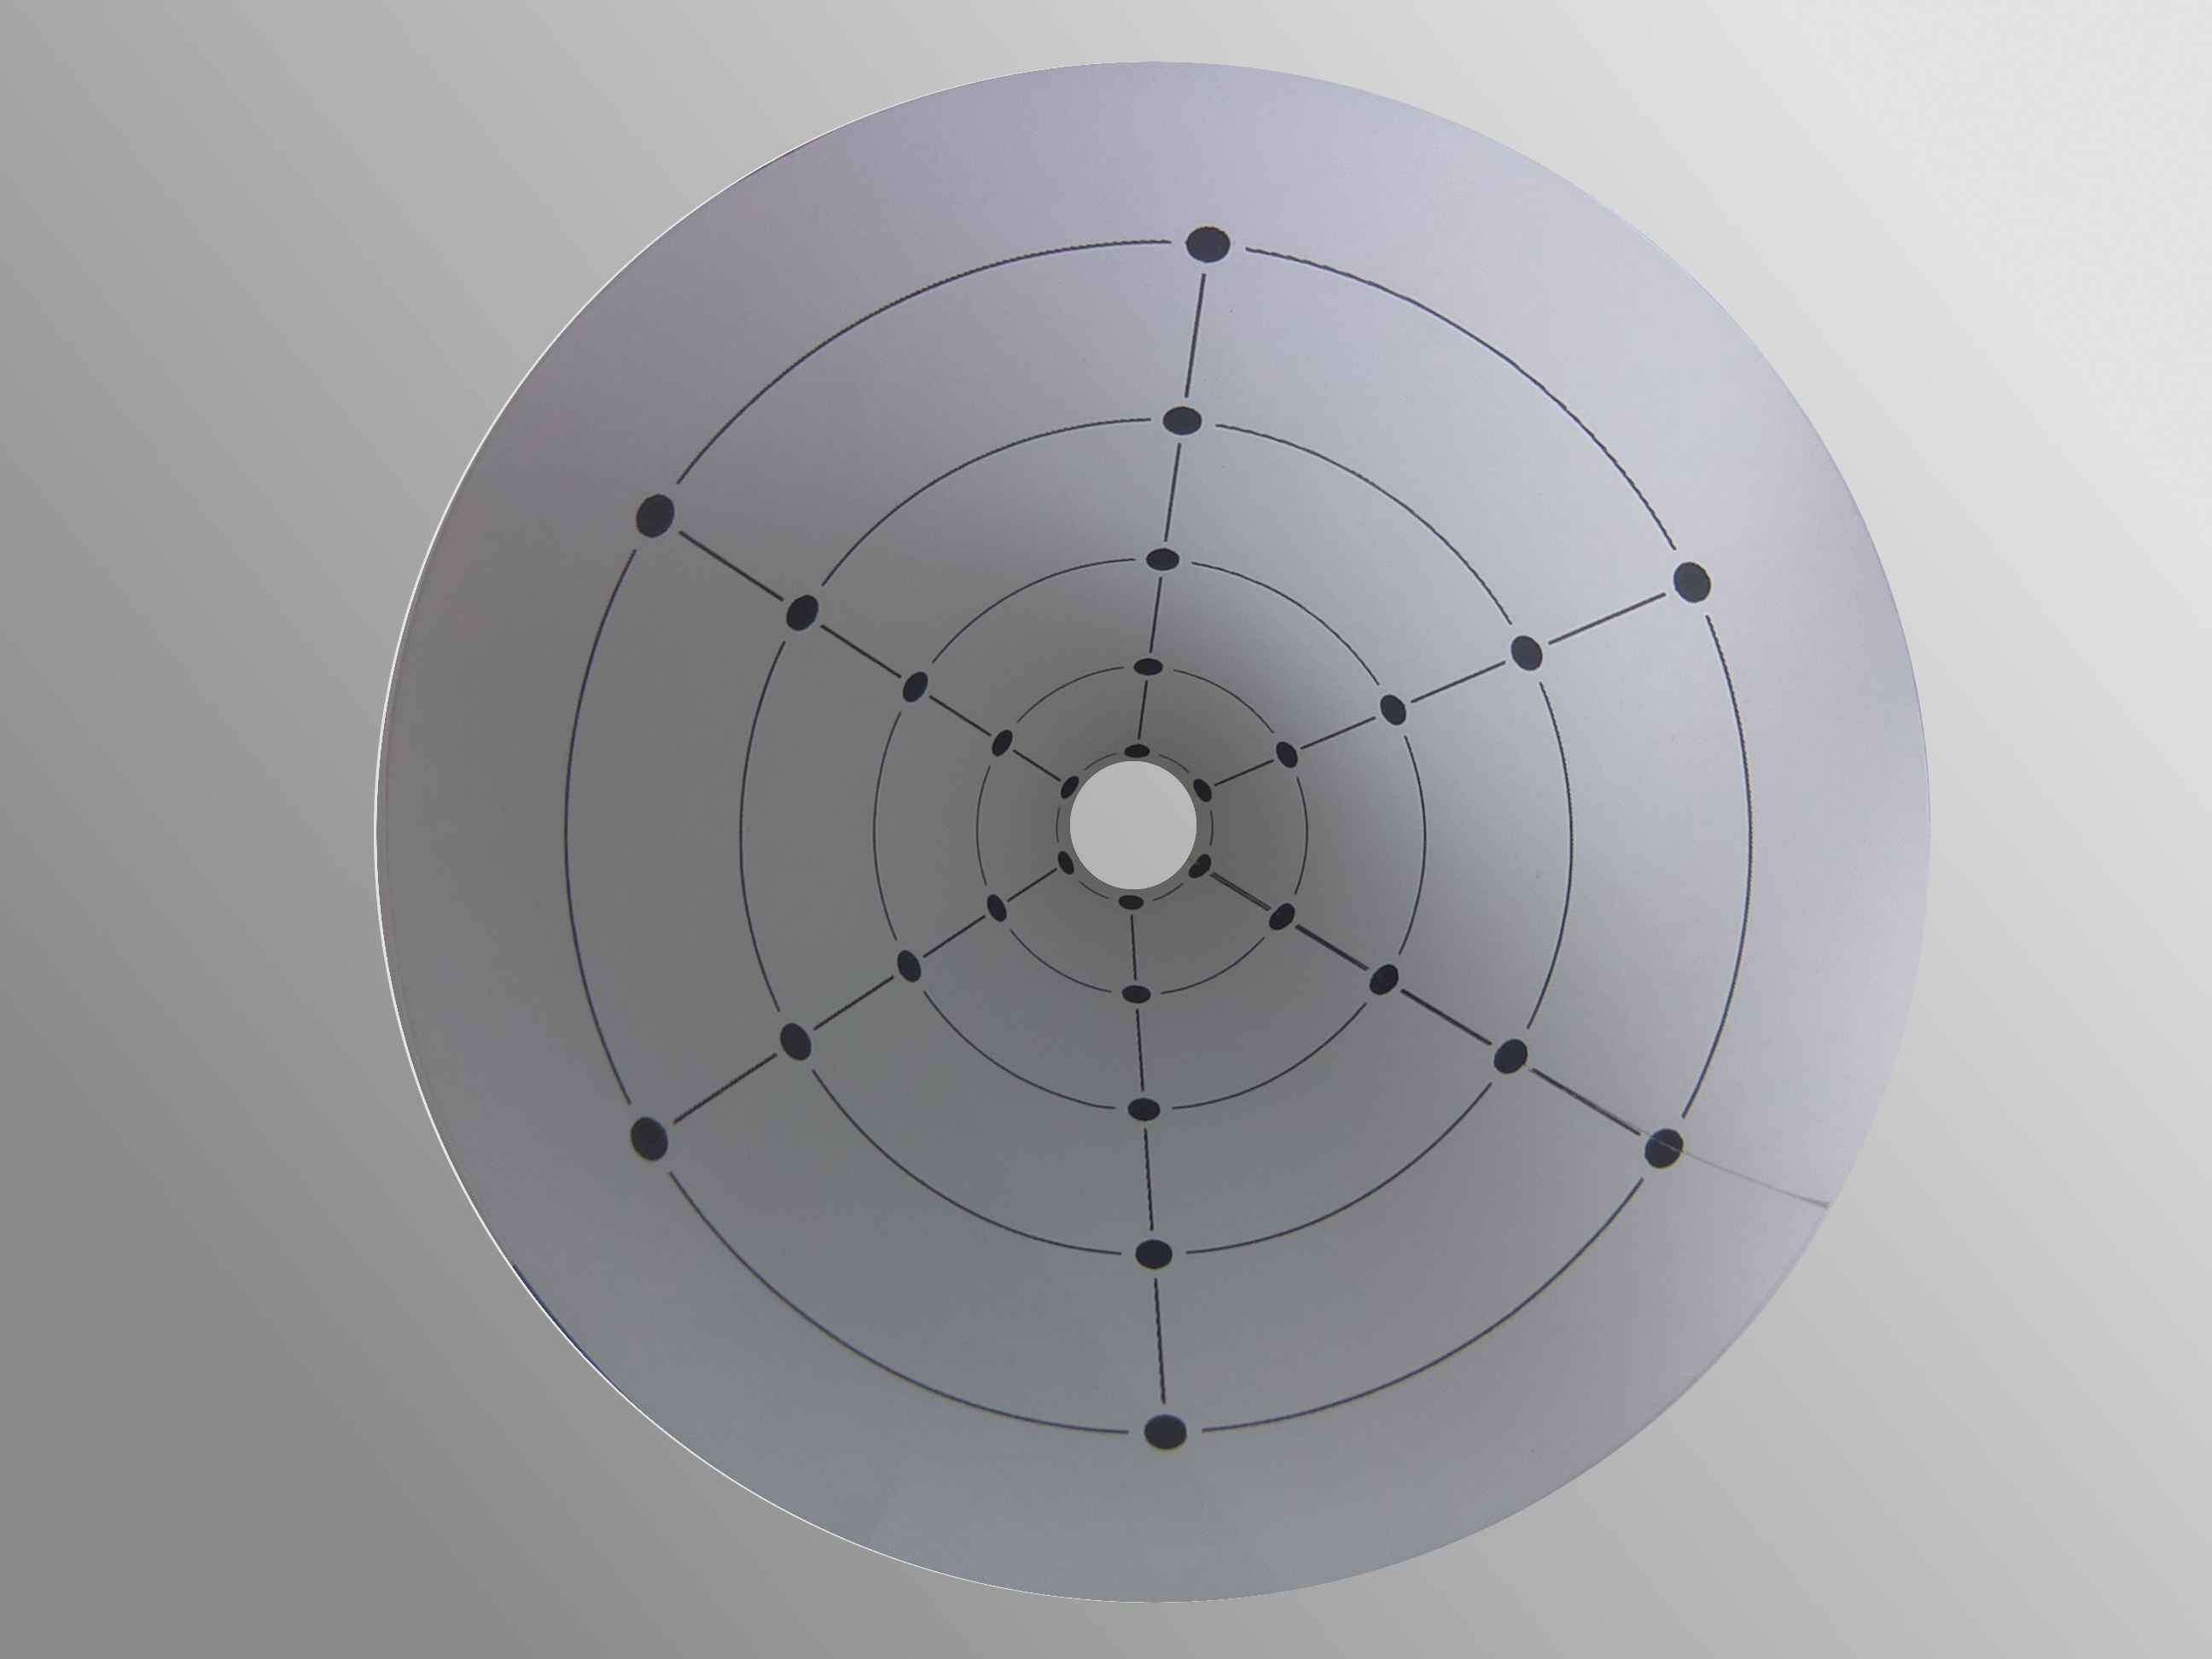
\includegraphics[width=.9\textwidth]{images/coneRasp.jpg}
		\caption{Grauwertbild}
	\end{subfigure}%
	\begin{subfigure}{.5\textwidth}
		\centering
		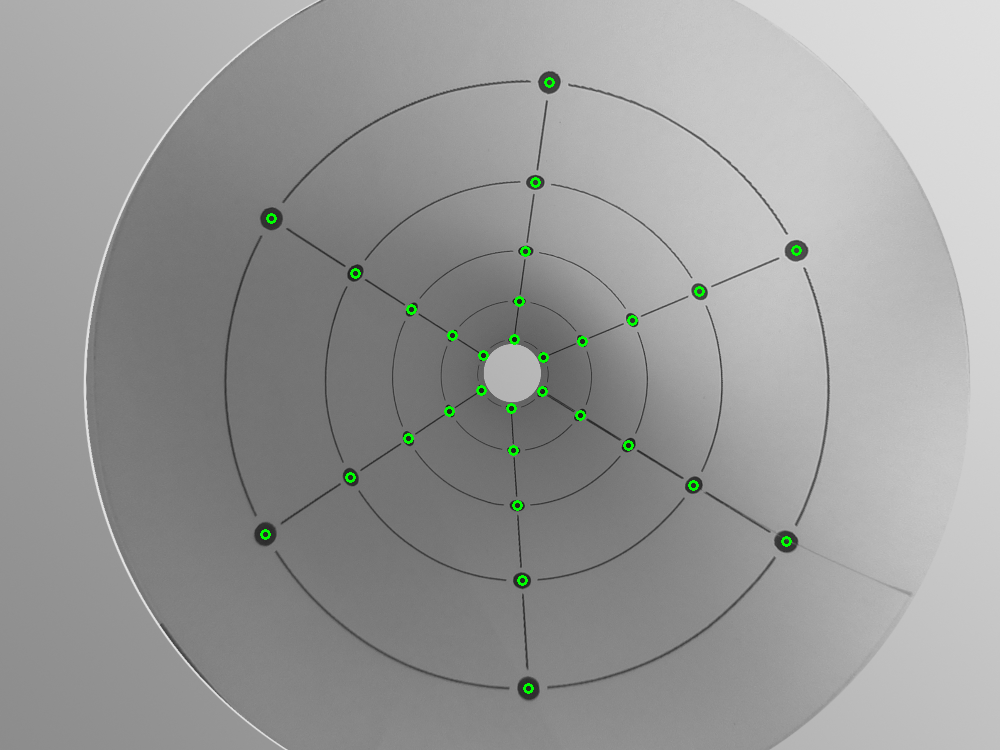
\includegraphics[width=.9\textwidth]{images/coneRaspDetectedDots.png}
		\caption{Grauwertbild und detektierte Blobs (rot)}
	\end{subfigure}
	\caption{Detektion der Samples}
	\label{fig:blobDetect}
\end{figure}


\section{Ellipsen-Detektion}
\label{s:ellipseDetection}

\subsection{RANSAC}
Nachdem die Sample-Positionen bestimmt wurden, muss für jeden Sample entschieden werden, auf welcher der Kreislinien es liegt. Da die Kreise, bedingt durch perspektivische Verzerrung, zu Ellipsen werden, wird eine Verfahren
benötigt, dass Ellipsen erkennt.



\begin{figure}[!htb]
	\centering
	\begin{subfigure}{.5\textwidth}
		\centering
		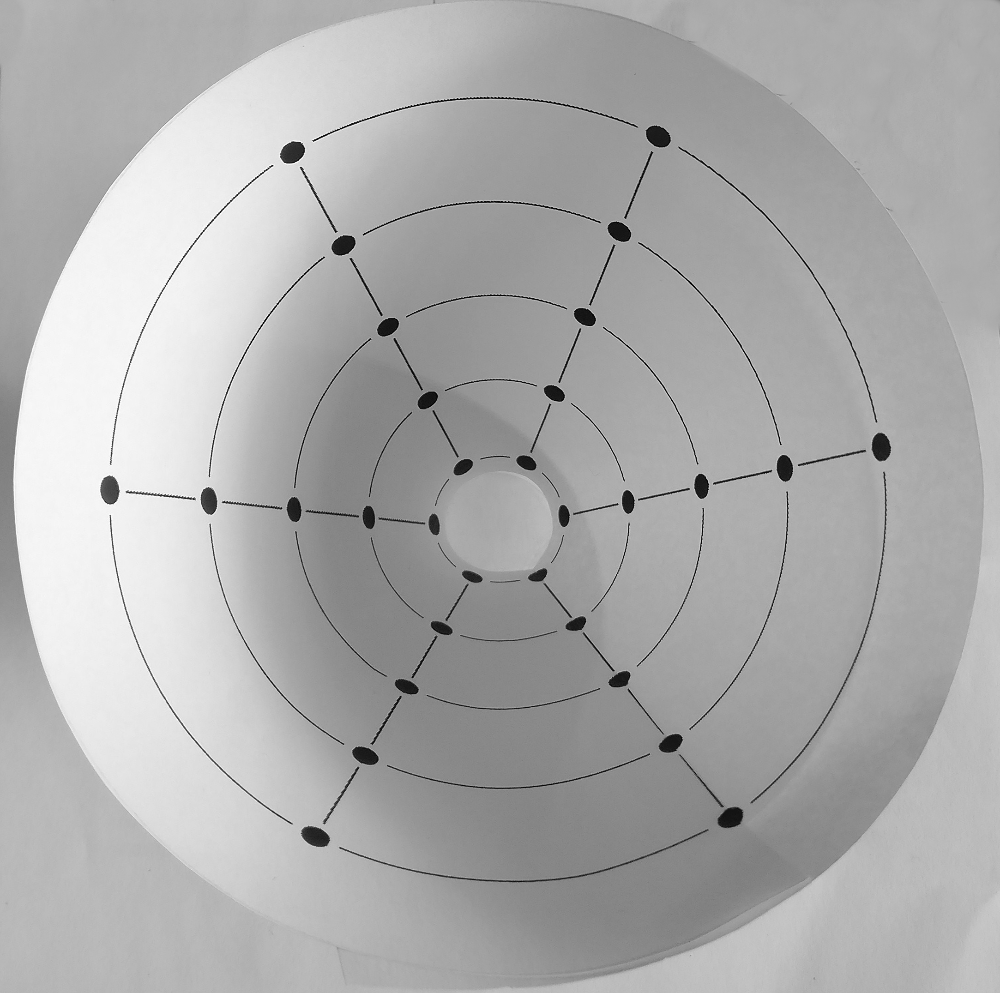
\includegraphics[width=.9\textwidth]{images/grey.png}
		\caption{Grauwertbild}
		\label{fig:beforeCanny}
	\end{subfigure}%
	\begin{subfigure}{.5\textwidth}
		\centering
		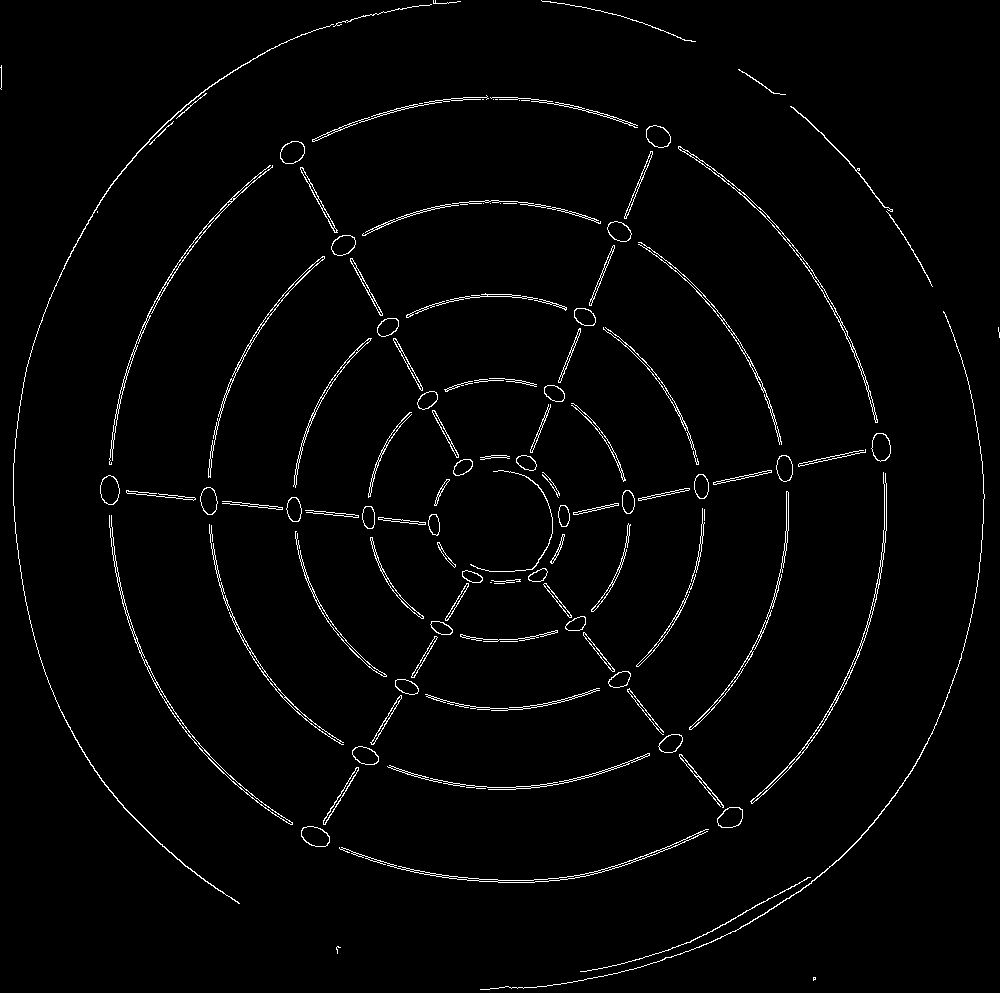
\includegraphics[width=.9\textwidth]{images/canny.png}
		\caption{Kantenbild}
		\label{fig:afterCanny}
	\end{subfigure}
	\caption{Canny-Kantendetektion}
	\label{fig:canny}
\end{figure}

Zunächst werden die Kanten mit Hilfe von Canny \cite{Canny1986} detektiert (siehe Abbildung \ref{fig:canny}).
Anschließend versuchen wir möglichst genau das Zentrum der innersten Ellipsen zu schätzen.
Wir benutzen dafür Hough-Transformationen (siehe Kapitel \ref{s:hough}), um Linien im Kantenbild zu detektieren.
Es werden anschließend die Schnittpunkte aller Liniensegmente bestimmt. Auf Grund der perspektivischen Verzerrung, schneiden sich die Liniensegmente nicht in einem Punkt.
Darüber hinaus werden, auf Grund der Liniendicke auf dem Kalibrierungsmuster, durch Canny viele Linien als doppelte Linien gekennzeichnet\footnote{Stellt man sich ein relativ breites Liniensegment vor, so gibt es einmal den Übergang vom Hintergrund auf die Linie, sowie den Übergang von der Linie wieder auf den Hintergrund}. Auch ein inhomogener Hintergrund, erschwert die Ermittlung eines Mittelpunkts. Befinden sich Objekte im Hintergrund, werden durch die Kantendetektion auch deren Kanten ermittelt. Die Hough-Transformation detektiert nun auch außerhalb des Kalibrierungsmusters Linien. Die Schnittpunkte mit solchen Linien können beliebig stark von dem eigentlichen Mittelpunkt abweichen. Würde man an dieser Stelle beispielsweise den Mittelwert aller Schnittpunkte (elementweise) berechnen, könnten solche Ausreißer die Lokalisierung des Mittelpunkts erheblich verschlechtern.

Um also möglichst robust einen Kandidaten auszuwählen, wird zuerst der Median der $x$-Koordinaten der Schnittpunkte und dann der Median der $y$-Koordinaten bestimmt. Die erhaltenen Koordinaten bilden den Schnittpunkt, wie in Abbildung \ref{fig:houghLines} beispielhaft zu sehen.

\begin{figure}[!htb]
	\centering
	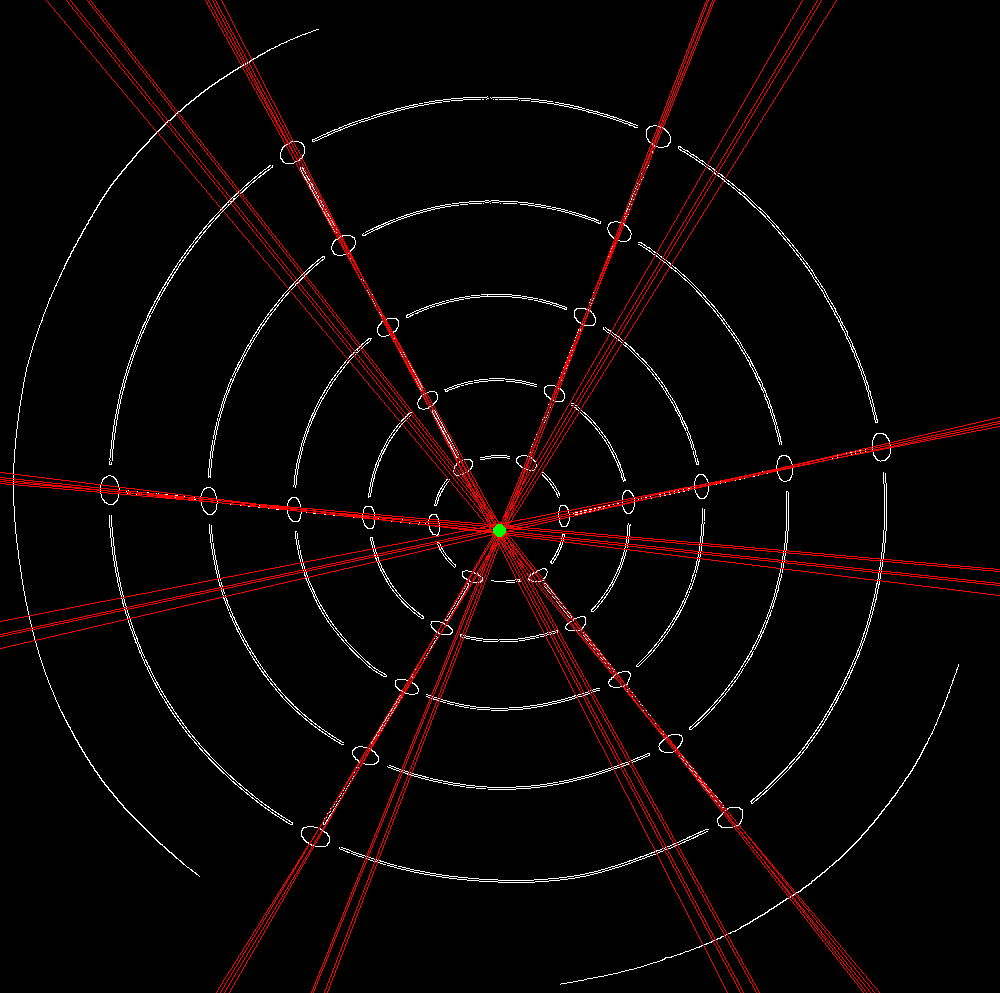
\includegraphics[scale=.25]{images/houghLines.png}
	\caption{Hough-Transformation zur Linien-Detektion (rot) und bestimmter Schnittpunkt (grün) }
	\label{fig:houghLines}
\end{figure}

Von diesem Schnittpunkt aus werden nun, in einer vorher definierte Anzahl, gleichmäßig, in alle Richtungen Strahlen ausgesendet.
Trifft ein Strahl ein weißes Pixel, wird dessen Position gekennzeichnet, trifft er den Rand des Bildes, wird er ignoriert. In Abbildung \ref{fig:rayCastWOE} sind beispielhaft die getroffenen weißen Pixel und der zugehörige Aussendepunkt eingezeichnet.

\begin{figure}[!htb]
	\centering
	\begin{subfigure}{.5\textwidth}
		\centering
		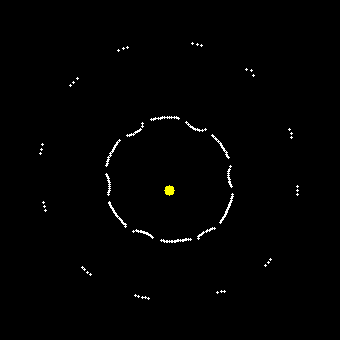
\includegraphics[width=.9\textwidth]{images/rayCast0.png}
		\caption{bestimme Pixel-Positionen}
		\label{fig:rayCastWOE}
	\end{subfigure}%
	\begin{subfigure}{.5\textwidth}
		\centering
		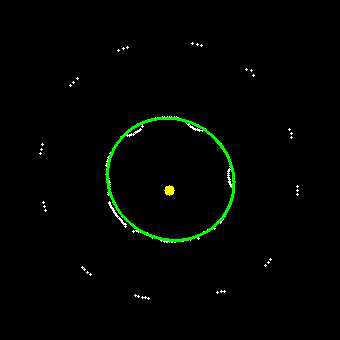
\includegraphics[width=.9\textwidth]{images/rayCast0Ellipse.png}
		\caption{bestimme Ellipse (grün)}
		\label{fig:rayCastWE}
	\end{subfigure}
	\caption{Ellipsendetektion: bestimme Pixel-Positionen (weiß), Aussendepunkt (gelb)}
	\label{fig:rayCast}
\end{figure}

Mit Hilfe der Postionen der weißen Pixel, schätzen wir anschließend mittels RANSAC (siehe Kapitel \ref{s:ransac}) eine Ellipse.

Es wird konkret wiederholt für sechs zufällig ausgewählte Punkte das lineare Gleichungssystem
\[
\begin{pmatrix}
x_1^2 & y_1^2 & x_1y_1 & x_1 & y_1 & 1\\
\vdots &\vdots & \vdots & \vdots &\vdots & \vdots\\
\vdots &\vdots & \vdots & \vdots &\vdots & \vdots\\
x_6^2 & y_6^2 & x_6y_6 & x_6 & y_6 & 1
\end{pmatrix} \begin{pmatrix}
a \\ b \\ c \\ d \\ e \\ f
\end{pmatrix} = \begin{pmatrix}
0 \\ 0 \\ 0 \\ 0 \\ 0 \\ 0
\end{pmatrix}
\]

gelöst, was auf der Gleichung \ref{eq:ellipseQuadratic} aus Kapitel \ref{s:ellipse} basiert. Wir benutzen hier die Polynomschreibweise einer Ellipse, da diese im Gegensatz zu der Form $(x_0,y_0,a,b,\phi)$ linear ist. Das Gleichungsystem ist also ein lineares Gleichungssystem und kann mit herkömmlichen Methoden der Numerik gelöst werden. Ein Nachteil dieses Ansatzes ist jedoch, dass nicht alle Werte für $(a,b,c,d,e,f)$ eine nicht entartete reele Ellipse definieren. Nach dem Lösen muss demnach geprüft werden, ob es sich tatsächlich um eine Ellipse handelt.
Diese wird dann mittels Hauptachsentransformation, wie in Kapitel \ref{s:ellipse} beschrieben, in die Ellipsenform $(x_0,y_0,a,b,\phi)$ umgewandelt.

Um die, für RANSAC benötigte, Distanz zu berechnen, wird das Verfahren aus Kapitel \ref{sc:distPointEllipse} genutzt, was die exakte euklidische Distanz eines Punktes zu einer Ellipse in der Form $(x_0,y_0,a,b,\phi)$ approxmiert.
Ein Verfahren wie das Verfahren der kleinsten Quadraten anstelle von RANSAC funktioniert hier nicht, da die weißen Pixel bezüglich einer zu bestimmenden Ellipse, ausreißerbehaftet sind. Wird zum Beispiel auf Grund schlechter Lichtverhältnisse eine Kreislinie nicht deutlich aufgenommen, kann es in dem Kantenbild dazu kommen, dass Kreislinien nicht zusammenhängend sind und folglich treffen die ausgesendeten Strahlen teilweise die nächst äußere Kreislinie. Diese Problem ist in Abbildung \ref{fig:rayCastR} zu sehen. Man sieht, dass die Anzahl der Pixel, auf der Ellipse, dessen Parameter wir schätzen wollen, im Vergleich zur Abbildung \ref{fig:rayCast} stark abgenommen hat. Die Strahlen treffen vermehrt auf die nächste äußere Ellipse. Die Ausreißeranzahl nimmt stark zu.

Da die Laufzeit nicht im Vordergrund steht, kann eine großzügige Schätzung des Fehleranteils von $\epsilon = 0.4$ mit einer gewünschten Wahrscheinlichkeit $p = 0.9999$ gewählt werden, was zu einer Mindestanzahl an Iterationen von circa $200$ führt (siehe Kapitel \ref{s:ransac}). Die letztendlich bestimmten Ellipsen sind beispielhaft in Abbildung \ref{fig:detectedEllipses} zu sehen. %Die Ellipsen beschreiben die Samples teilweise nicht optimal, wie es zum Beispiel bei der äußersten Ellipse der Fall ist. Da wir die Ellipsen zunächst nur benutzten, um eine Zuordnung der Samples zu erhalten, reicht


\begin{figure}[!htb]
	\centering
	\begin{subfigure}{.5\textwidth}
		\centering
		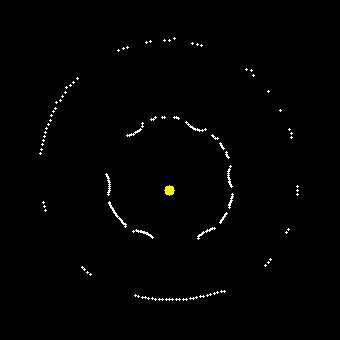
\includegraphics[scale=.6]{images/rayCastRobust.png}
		\caption{bestimme Pixel-Positionen}
		\label{fig:rayCastRWOE}
	\end{subfigure}%
	\begin{subfigure}{.5\textwidth}
		\centering
		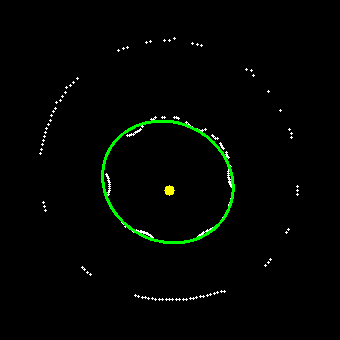
\includegraphics[scale=.6]{images/rayCastRobustEllipse.png}
		\caption{bestimme Ellipse (grün)}
		\label{fig:rayCastRWE}
	\end{subfigure}
	\caption{Ellipsendetektion bei Ausreißern}
	\label{fig:rayCastR}
\end{figure}


\begin{figure}[!htb]
	\centering
	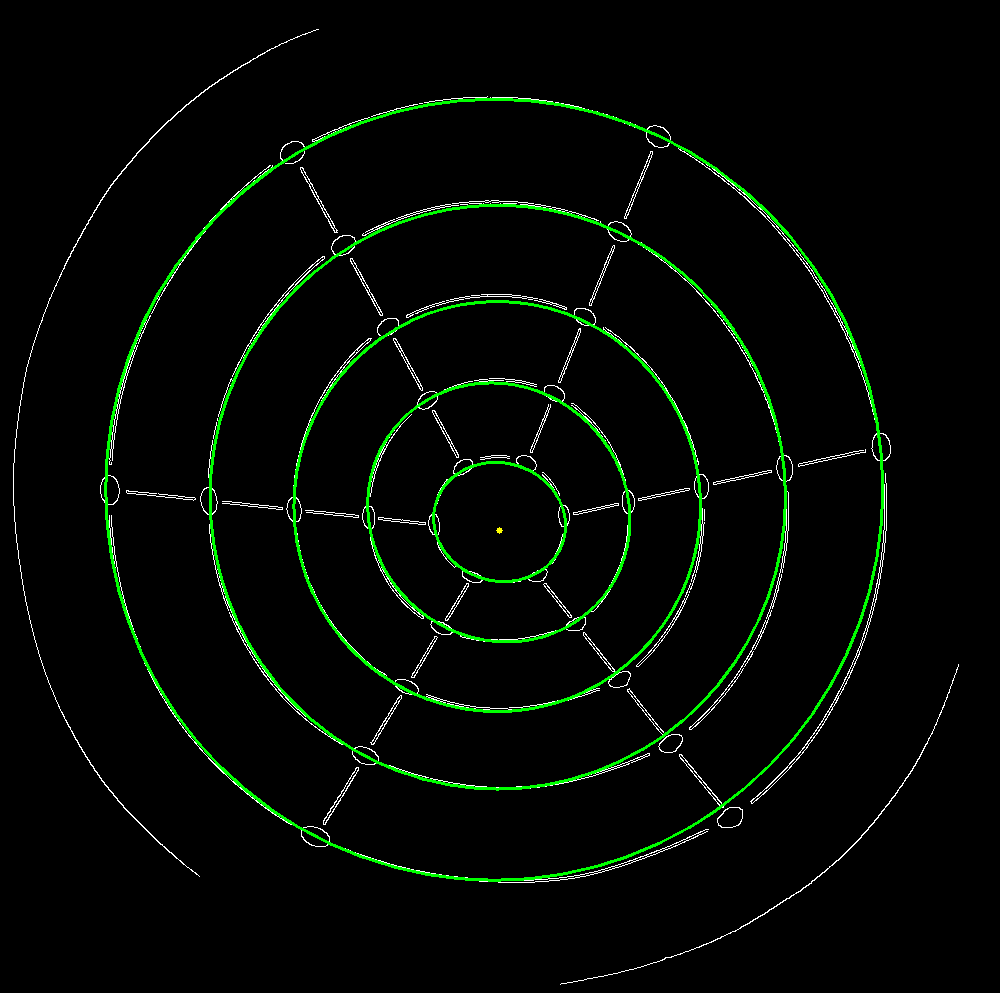
\includegraphics[scale=.25]{images/detectedEllipses.png}
	\caption{detektierte Ellipsen}
	\label{fig:detectedEllipses}
\end{figure}


\subsection{Analytical Deformable Templates}

Als Alternative zu RANSAC können die Ellipsen auch mittels \textit{Analytical Deformable Templates} (siehe Kapitel \ref{s:anaDef}) detektiert werden. Wir betrachten dazu folgende Funktion, deren Nullstellen eine um $\theta$ gedrehte Ellipse, mit Zentrum $(x_0,y_0)$ und Haupt- und Nebenachse $a$ und $b$ beschreiben.
\[
	G(x,y) = \frac{((x - x_0)\cos\theta + (y - y_0)\sin\theta)^2}{a^2} + \frac{((x - x_0)\sin\theta - (y - y_0)\cos\theta)^2}{b^2} - 1
\] %%
Die Ellipse lässt sich, wie in Kapitel \ref{s:cone}, auch parametrisch beschrieben durch die Funktion
\[
H(\phi) = \begin{pmatrix}x_0 + a\cos\phi\cos\theta - b\sin\phi\sin\theta \\
y_0 + a\cos\phi\sin\theta + b\sin\phi\cos\theta\end{pmatrix}
\] %%
mit $\phi \in [0,2\pi)$

Wir konstruieren nun eine Energiefunktion
\[
	E = E_M + E_A + E_S,
\]
die sich zusammensetzt aus einem Term $E_M$, der die Kantenstärke auf dem Ellipsenrand maximiert, sowie einem Term $E_A$ der die Winkelähnlichkeit zwischen Ellipsennormale und Gradientenrichtung des Bildes maximiert. Darüber hinaus fügen wir einen Term $E_S$ hinzu, der die Ellipse schrumpfen lässt.

Konkret sehen die Terme wie folgt aus
\begin{equation}\label{eq:deformTerms}
	\begin{aligned}
		E_M &= -\alpha\frac{1}{n}\sum_{i=0}^{n-1}I_M(p_i) \\
		E_A &= \beta\frac{1}{n}\sum_{i=0}^{n-1}\left(I_O(pi) - \atant{\left(\frac{\partial G}{\partial y}(p_i), \frac{\partial G}{\partial x}(p_i)\right)}\right)^2 \\
		E_S &= \gamma\frac{1}{n}\sum_{i=0}^{n-2}\left(p_i - p_{i+1}\right)^2,
	\end{aligned}
\end{equation}

wobei $n$ die Anzahl der Punkte auf dem Ellipsenrand sind. $p_i$ ist definiert als der $i$-te Punkt auf der Ellipse, also als $H(\phi_i)$ mit $\phi_i = \frac{i}{n}\cdot2\pi ~\forall i = 0,\dotsc,n-1$.
Der Term $I_M(p_i)$ ist definiert als $I_M(p_i) = \sqrt{I_x(p_i)^2 + I_y(p_i)^2}$, wobei $I_x$, sowie $I_y$ für die diskreten partiellen Ableitungen nach $x$ respektive $y$ stehen. Durch $I_M(p_i)$ wird somit die Kantenstärke in Punkt $p_i$ charakterisiert. Der Term $I_O(p_i)$ ist definiert als $I_O(p_i) = \atano\left(\frac{I_y(p_i)}{I_x(p_i)}\right)$
und beschreibt somit die Gradientenrichtung der Kanten.

Man wählt dabei als Startwert eine Ellipse, deren Zentrum dem Bildzentrum entspricht und deren Hauptachse und Nebenachse möglichst groß sind ($a = w/2$ und $b = h/2$ für ein Bild mit Breite $w$ und Höhe $h$) und bestimmt dann numerisch ein Minimum der Funktion. Der Term $E_M$ wird minimal, wenn entlang der Ellipse die Kantenstärke groß ist. Der Term $E_A$ wird minimal wenn die Winkel der Normalenvektoren ähnlich zu denen der Kanten sind und $E_S$ wird minimal, wenn die Distanz aufeinanderfolgender Ellipsepunkte klein wird, also der Ellipsenumfang klein wird. Der Term lässt die Ellipse also schrumpfen. $\alpha, \beta$ und $\gamma$ steuern hierbei den Einluss der einzelnen Terme. Das Minimum der Funktion sollte die äußerste Ellipse im Kalibirierungsmuster sein. Anschließend wird diese Ellipse vom Bild entfernt und man sucht wiederholt Minima der Funktion bis alle Ellipse detektiert wurden.




\section{Zuordnung der Punkte}
\label{s:pointMapping}
Nach der Bestimmung der Ellipsen muss jede Sample-Position der zugehörigen Kreislinie, sowie dem zugehörigen Liniensegment zugeordnet werden, um seine Position auf dem Kegel bestimmen zu können.
Zunächst wird für jeden Punkt diejenige Kreislinie ausgewählt, dessen zugehörige Ellipse die kürzeste Distanz zu ihm hat, wie in Abbildung \ref{fig:ellipseMapping} zu sehen. Die Farbe eines Samples entspricht hier der Farbe der zugeordneten Ellipse.

Um nun die Samples auch ihren Liniensegmenten zuzuordnen, wird zunächst der Mittelpunkt der Samples auf der innersten Ellipse bestimmt. Anschließend werden die Samples auf der innersten Ellipsen nach dem Winkel der Verbindungslinien zwischen Sample und Mittelpunkt mit der $x$-Achse sortiert.
Die restlichen Samples können nicht nach dem gleichen Schema sortiert werden, da der bestimme Mittelpunkt nicht der genaue Schnittpunkt aller Liniensegmente ist.
Das Problem ist in Abbildung \ref{fig:sampleMappingProblem1} am Beispiel eines Liniensegments für zwei Samples illustriert. Das bestimme Zentrum $C$ liegt nicht auf der Verlängerung des Liniensegments.  Die Winkel der Verbindungslinien zum Zentrum $\alpha_1$, sowie $\alpha_2$ unterscheiden sich. Bei einer Sortierung nach Winkel ist nicht mehr gewährleistet, dass die Samples zu einer Verbindungslinie gehören, da die Winkel der Samples eines Liniensegments beliebig voneinander abweichen können.  Damit dieses Verfahren funktioniert müsste die Situation aus Abbildung \ref{fig:sampleMappingProblem2} für alle Liniensegmente gelten, das heißt der Winkel (hier: $\beta$) ist für alle Verbindungslinien identisch.

\begin{figure}[!htb]
	\centering
	\begin{subfigure}{.6\textwidth}
		\centering
		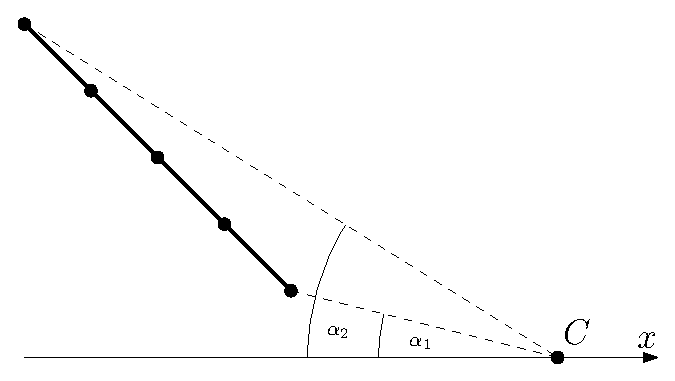
\includegraphics[width=.9\textwidth]{images/sampleMappingProblem.eps}
		\caption{Zuordnung von Punkten zu Ellipsen}
		\label{fig:sampleMappingProblem1}
	\end{subfigure}%
	\begin{subfigure}{.4\textwidth}
		\centering
		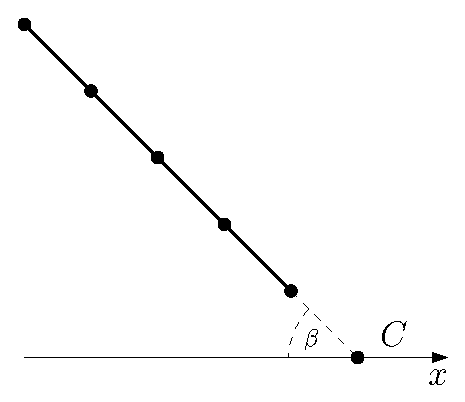
\includegraphics[width=.9\textwidth]{images/sampleMappingProblem2.eps}
		\caption{Zuordnung von Punkten zu Liniensegmenten}
		\label{fig:sampleMappingProblem2}
	\end{subfigure}
	\caption{Zuordnung von Punkten zu Ellipsen (links) und Liniensegmenten (rechts)}
	\label{fig:sampleMappingProblem}
\end{figure}

Stattdessen wird für jedes Sample auf den darauffolgenden Ellipsen das Sample auf der vorherigen Ellipse mit der kürzesten Distanz bestimmt.
Die Samples können nun entsprechend sortiert werden. Die zugeordneten Liniensegmente sind exemplarisch in Abbildung \ref{fig:lineMapping} zu sehen. Darüber hinaus lässt sich hier erkennen, dass das Liniensegment mit dem kleinsten Winkel zur $x$-Achse das erste Liniensegment (rot) ist. Das Liniensegment wird später unsere Bezugspunkt zur Entzerrung sein, also diejenige Kante, an der der Kegel entrollt wird.


\begin{figure}[!htb]
	\centering
	\begin{subfigure}{.5\textwidth}
		\centering
		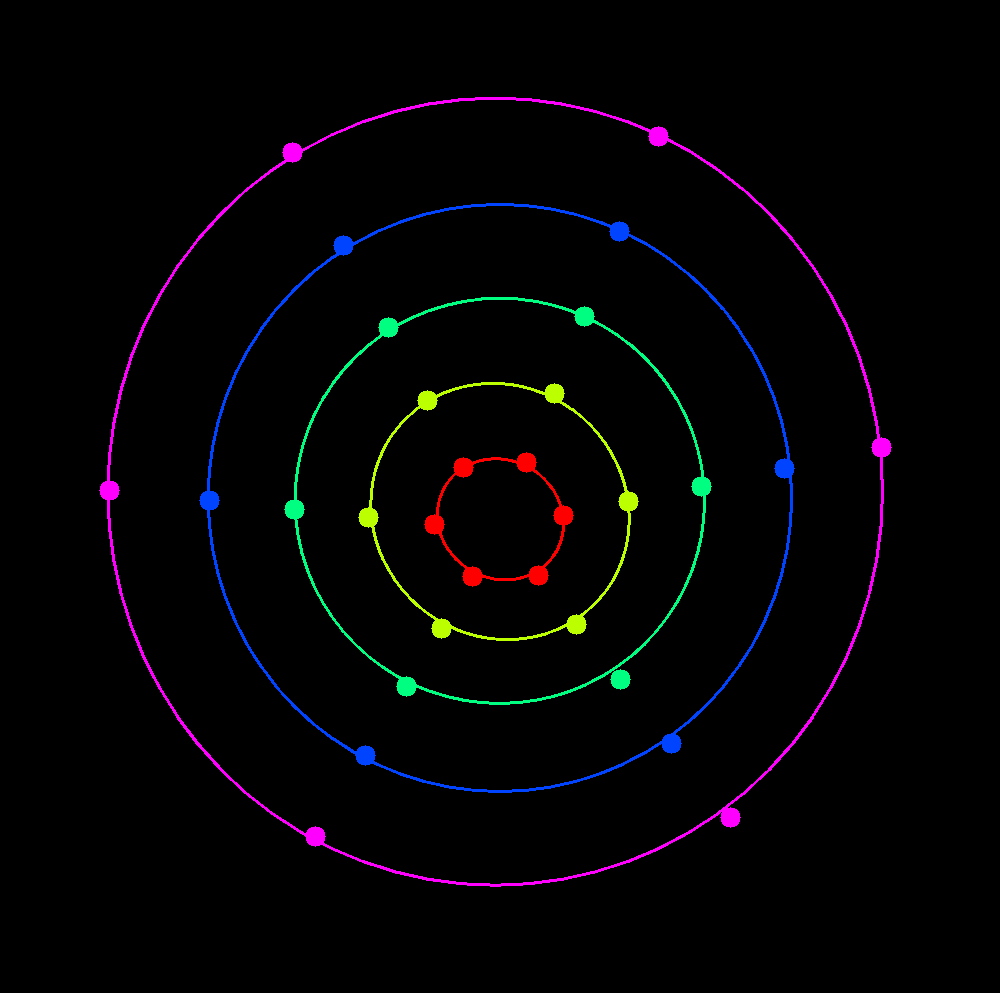
\includegraphics[width=.9\textwidth]{images/ellipseMapping.png}
		\caption{Zuordnung von Punkten zu Ellipsen}
		\label{fig:ellipseMapping}
	\end{subfigure}%
	\begin{subfigure}{.5\textwidth}
		\centering
		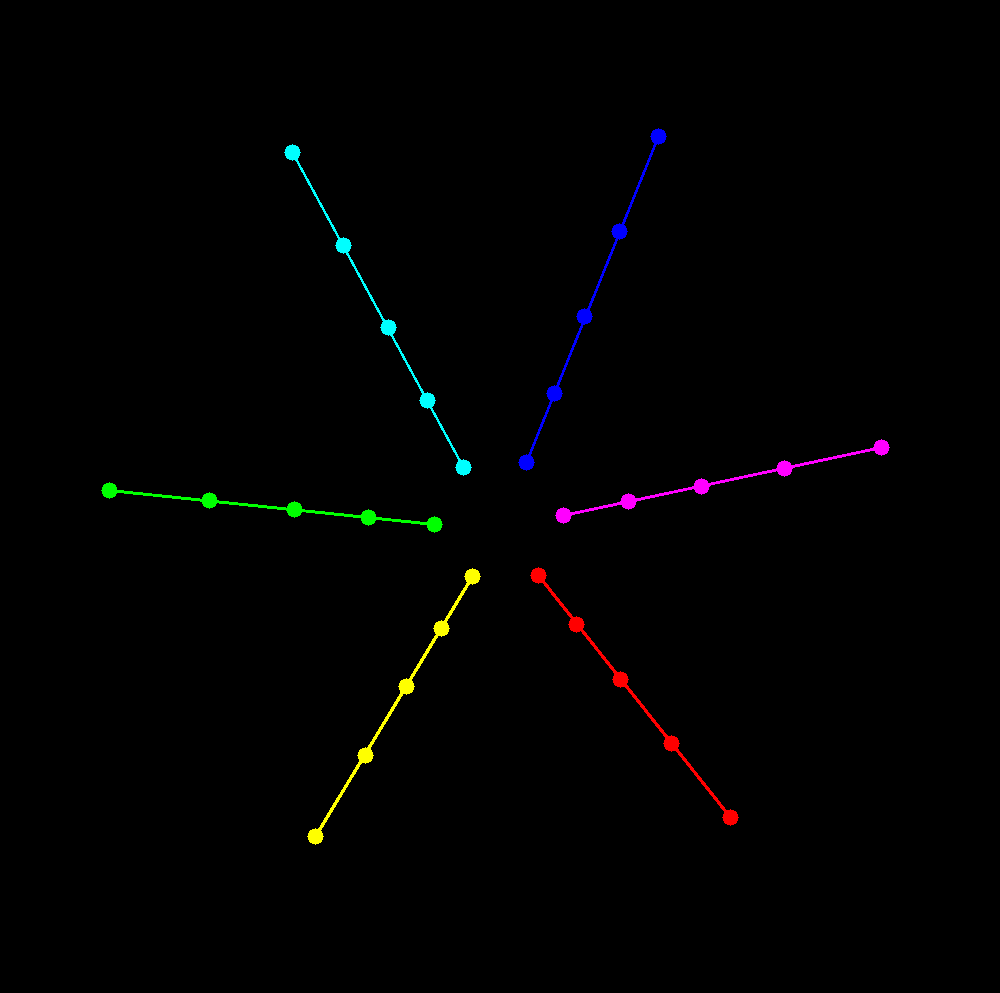
\includegraphics[width=.9\textwidth]{images/lineMapping.png}
		\caption{Zuordnung von Punkten zu Liniensegmenten}
		\label{fig:lineMapping}
	\end{subfigure}
	\caption{Zuordnung von Punkten zu Ellipsen (links) und Liniensegmenten (rechts) farblich sortiert: 1. rot, 2. gelb, 3. grün, 4. blau, 5. magenta}
	\label{fig:mapping}
\end{figure}


Mit Hilfe dieser Zuordnung schätzen wir die Ellipsen erneut. Die Samples dienen als Messpunkte und wir nutzen das Verfahren der kleinsten Quadrate, da wir eine optimale Lösung für alle Samples anstreben.

\section{Weltkoordinaten bestimmen}
Wir können nun jedem Sample eine Kreislinie, sowie ein Liniensegment zuordnen. Damit wir Korrespondenzen zwischen den Samples und dem Kegel herstellen können, müssen wir im nächsten Schritt jedem Sample dreidimensionale Koordinaten auf der Kegeloberfläche zuweisen.

Mit Hilfe der Parametrisierung des Kegelstumpfs können wir die 3D-Koordinaten eines Samples folgendermaßen angeben:

Ohne Beschränkung der Allgemeinheit, seien die Ellipsen $i = 0,\dotsc,n - 1$ aufsteigend nach ihrer "`Größe"'\footnote{Etwas formaler, könnte man die Ellipsen hier nach ihrem Flächeninhalt sortieren. Für Ellipsen $E_0(x_0,y_0,a_0, b_0, \theta_0)$ und $E_1(x_1,y_1,a_1, b_1,\theta_1)$ gilt $E_0 \leq E_1$ g.d.w. $\pi\cdot a_0 \cdot b_0 \leq \pi \cdot a_1 \cdot b_1$} sortiert.
Außerdem seien die Liniensegmente $j = 0,\dotsc,m - 1$ aufsteigend nach Winkel mit der $x$-Achse, wie in Kapitel \ref{s:pointMapping} beschrieben, sortiert.
Eine Sample kann also eindeutig durch ein Tupel $(i,j) \in [0,n-1]\times [0,m-1]$ identifiziert werden und $(x_{ij},y_{ij},z_{ij})$ bezeichne seine Koordinaten im Weltkoordinatensystem.

Analog zur parametrischen Darstellung von Kegelstümpfen (Gleichung \ref{eq:paramFrustum}) in Kapitel \ref{s:cone} ergibt sich

\[
\begin{aligned}
x_{ij} &= r_i~cos \theta_j \\
y_{ij} &= h_i\\
z_{ij} &= r_i~sin \theta_j
\end{aligned}
\]
$\forall (i,j) \in [0,n-1]\times [0,m-1]$ mit
\[
\begin{aligned}
r_i &= r + \frac{i}{n - 1}\cdot(R - r) \quad&\forall i\in[0,n-1]\\
h_i &= \frac{i}{n - 1}\cdot\Delta H &\forall i\in[0,n-1]\\
\theta_j &= \frac{j}{m-1} \cdot  2\pi  &\forall j\in[0,m-1]
\end{aligned}
\] %%
enstprechend dem Aufbau des Kalibrierungsmusters.



\section{Entfaltung}
\label{s:unfolding}
Die eigentliche Entfaltung des Kegels kann mit zwei unterschiedlichen Ansätzen realisiert werden.
Die erste Möglichkeit ist die Vorwärtsentfaltung. Hierbei wird für jedes Pixel auf dem Kegelbild eine 3D-Koordinate durch geeignete Interpolation bestimmt und dann auf die Mantelfläche abgebildet. Beim zweiten Ansatz, der Rückwärtsentfaltung, wird ein Punkt von der Mantelfläche zurück auf den Kegel abgebildet und von dort mit einer Projektionsmatrix auf die Bildebene projiziert und dann interpoliert.

\subsection{Vorwärtsentfaltung}
Bei der Vorwärtsentfaltung muss wie oben erwähnt zu jedem Pixel die zugehörige 3D-Koordinate im Weltkoordinatensystem berechnet werden. Da bisher jedoch nur die Positionen der Samples bekannt sind muss hier entsprechend interpoliert werden.

Zunächst betrachten wir diejenigen Pixel, die sich weder auf einer Kreislinie, noch auf einem Liniensegment befinden. Es gibt zu einem Pixel $P$ also immer vier Sample-Nachbarn $(b_l, b_r, t_r, t_l)$. Diese Situation ist in Abbildung \ref{fig:radialInterpolation} illustriert.

Nachdem die vier Nachbarn bestimmt wurden, können wir im ersten Schritt die Abstände $d_1$ und $d_2$ von Pixel $P$ zu inneren Ellipse $E_b$, respektive äußeren Ellipse $E_t$ berechnen. Mithilfe dieser Abstände kann nun eine "`Interpolationsellipse"' $E_1$ definiert werden als
\begin{equation*}
	E_{int} = \left(\frac{d_1}{d_1 + d_2}\right) \cdot E_t + \left(\frac{d_2}{d_1 + d_2}\right) E_b,
\end{equation*}

wobei eine Multiplikation mit einem Skalar alle Charakteristika einer Ellipse skaliert. Der Drehwinkel $\theta$ wird hierbei bei $2\pi$ umgebrochen. Eine Addition geschieht elementweise. Im nächsten Schritt wird der Schnittpunkt $L$ mit dem Liniensegment $\overline{b_lt_l}$, sowie der Schnittpunkt $R$ mit dem Liniensegment $\overline{b_rt_r}$ bestimmt.

Da sich $t_l$, $L$ und $b_l$ nun auf einem gemeinsamen Liniensegment befinden, kann bezüglich der Weltkoordinaten linear interpoliert werden. Analoges gilt für $t_r$,$R$ und $b_r$.
Die interpolierte Weltkoordinaten von $L$, sowie $R$ bezeichnen wir als $L_W$ und $R_W$

Die drei Punkte $(L, P, R)$ befinden sich auf der Interpolationsellipse und somit können die  Winkel $(\phi_L, \phi_P, \phi_R)$ bezüglich des gemeinsamen Ellipsenkoordinatensystems bestimmt werden. Dazu transformieren wir die Ellipse, sowie den Punkt in das Koordinatensystem, indem sich die Ellipse im Ursprung und ihre Hauptachsen achsenausgerichtet sind. Die Abbildung ist rigide, erhält also Längen und Winkel. Die Ellipse kann nun parametrisch beschrien werden als
\[
\begin{pmatrix}x \\ y\end{pmatrix} = \begin{pmatrix}a\cos\phi \\
b\sin\phi\end{pmatrix}
\] %%
mit $\phi \in [0, 2\pi)$ und der Haupt- und Nebenachse $a$, beziehungsweise $b$. Zu einem gebenen Ellipsenpunkt $(x,y)$ können wir nun wieder den Winkel $\phi$ bezüglich der Ellipse bestimmen mit
\[
\phi = \atant \frac{y/b}{x/a} \bmod 2\pi.
\] %%

Analog zu oben werden nun die 3D-Koordinaten von $P$ als lineare Interpolation zwischen den bestimmen 3D-Koordinaten von $L$ und $R$ bestimmt. Als Interpolationsfaktor benutzen wir die Winkeldifferenzen
$\frac{\phi_L - \phi_P}{\phi_L - \phi_R}$. Wir erhalten für die Weltkoordinaten $P_W$ des Pixels $P$ insgesamt
\[
P_W = \left(\frac{\phi_L - \phi_P}{\phi_L - \phi_R}\right) R_W + \left(1 - \frac{\phi_L - \phi_P}{\phi_L - \phi_R}\right) L_W.
\]

\begin{figure}[!htb]
	\centering
	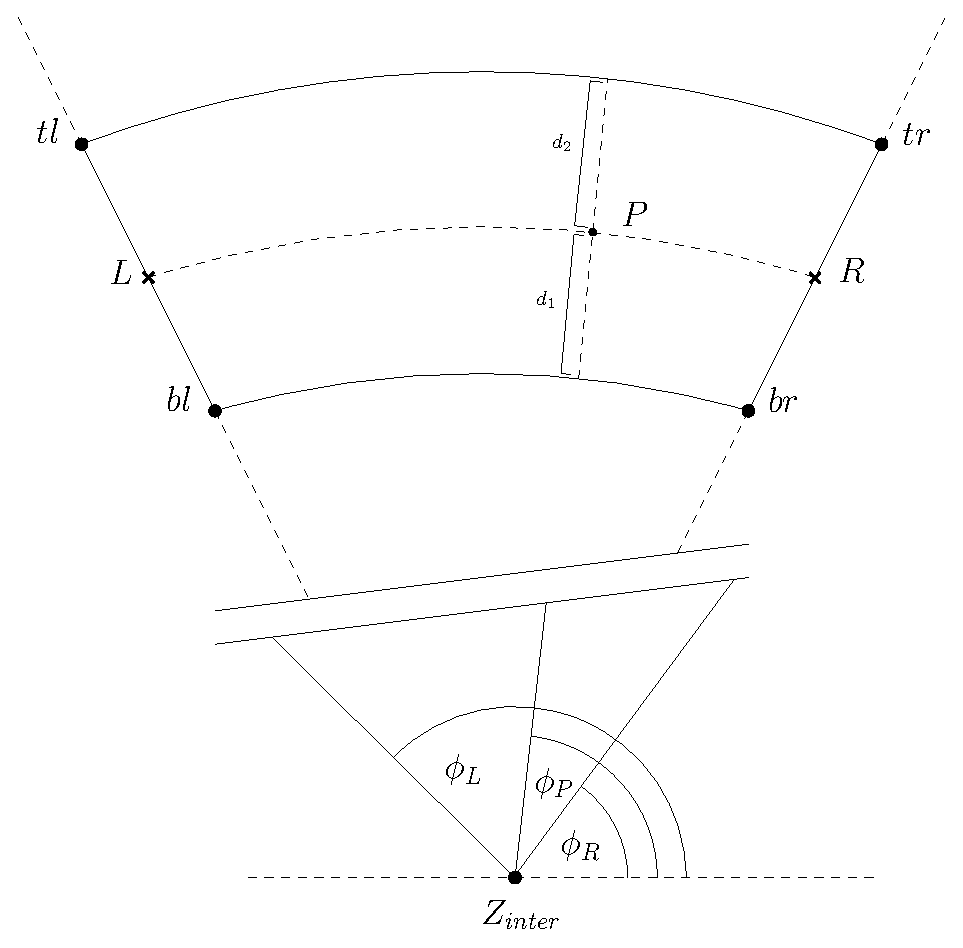
\includegraphics[scale=.6]{images/radialInterpolation.eps}
	\caption{Interpolation der 3D-Koordinaten mittels vier Sample-Nachbarn}
	\label{fig:radialInterpolation}
\end{figure}



Die Pixel, die sich auf Liniensegmenten befinden werden einfach linear interpoliert. Die Punkte, die sich auf Kreislinien befinden werden über Winkel interpoliert.

Jedes Pixel hat nun 3D-Koordinaten im Kegel erhalten. Mit Hilfe der konstruierten Abbildung \ref{eq:coneToLateral} aus Kapitel \ref{s:cone}, können wir nun die interpolierten Punkte auf die Mantelfläche abbilden und erhalten schließlich das entzerrte Bild (siehe Abbildung \ref{fig:forwardUnfold})



\begin{figure}[!htb]
	\centering
	\begin{subfigure}{.5\textwidth}
		\centering
		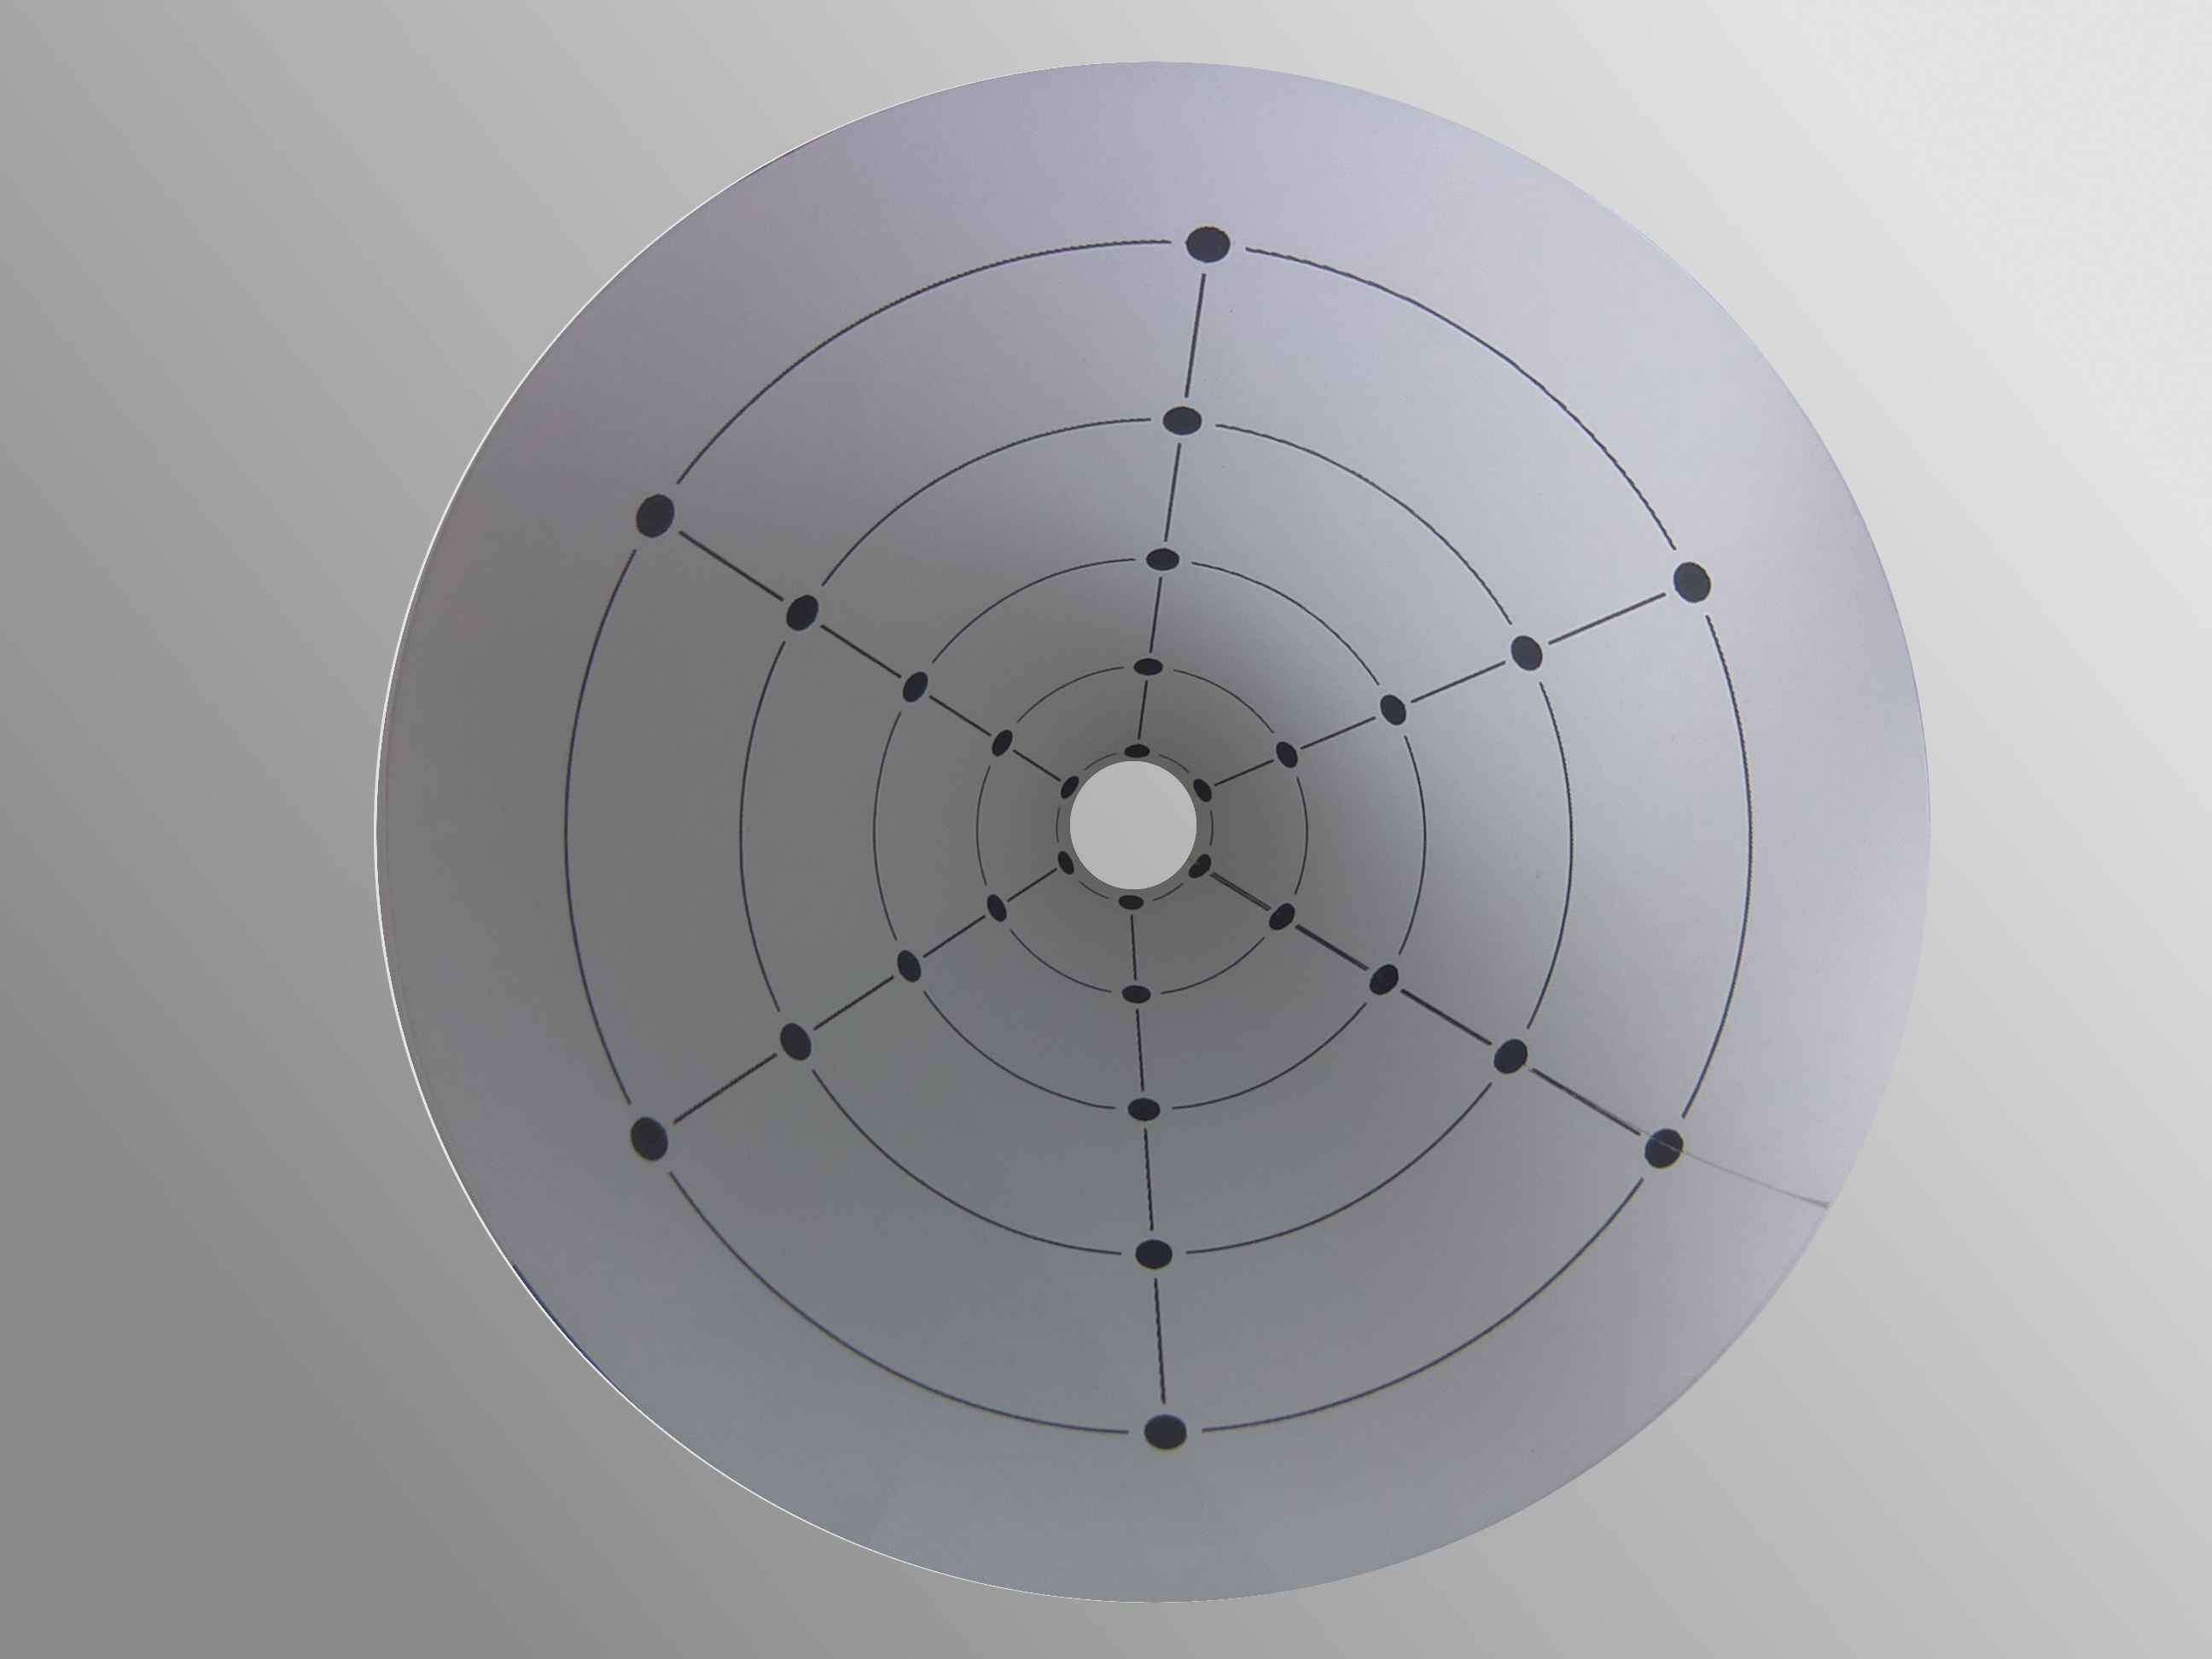
\includegraphics[width=.9\textwidth]{images/coneRasp.jpg}
		\caption{Ursprungsbild}
	\end{subfigure}%
	\begin{subfigure}{.5\textwidth}
		\centering
		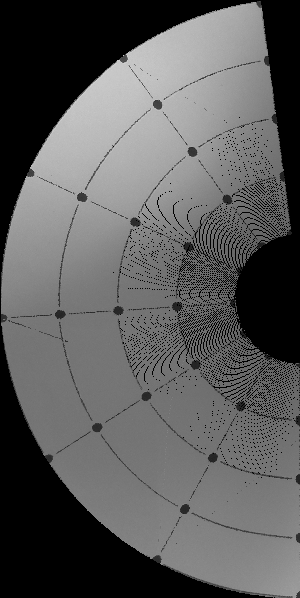
\includegraphics[angle=-90, width=.9\textwidth]{images/coneRaspUnWarpForward.png}
		\caption{entfaltetes Bild (um 90° im Uhrzeigersinn gedreht)}
	\end{subfigure}
	\caption{Vorwärtsentfaltung}
	\label{fig:forwardUnfold}
\end{figure}


\subsection{Rückwärtsentfaltung}
Bei der Rückwärtsentfaltung gehen wir von dem entzerrten Bild aus, dessen geometrische Eigenschaften aus der parametrischen Form der Mantelfläche des Kegels bekannt sind und versuchen rückwärts Pixelkandidaten im Ursprungsbild zu bestimmen.

Wir müssen zunächst für einen Punkt auf dem entzerrten Bild  dreidimensionale Koordinaten auf der Kegeloberfläche berechnen. Wir nutzen dafür die konstruierte Umkehrabbildung \ref{eq:LateralToCone} aus Kapitel \ref{s:cone}. Im nächsten Schritt müssen wir die erhaltenen Kegelkoordinaten auf das Ursprungsbild abbilden, um die Pixelkandidaten bestimmen zu können.

Wir konstruieren dafür eine Projektionsmatrix. Wie in Kapitel \ref{s:calib} nutzen wir die  Punktkorrespondenzen der Samples aus, um mittels \textit{Direct Linear Transformation} eine Projektionsmatrix zu bestimmen.
Wir erhalten somit die gewünschte Abbildung, die wir auf jede 3D-Koordinate anwenden, wodurch wir Bildkoordinaten erhalten. Im Allgemeinen, sind diese Koordinaten nicht ganzzahlig und wir müssen entsprechend interpolieren (linear oder bikubisch siehe Kapitel \ref{ch:analysis}).

\begin{figure}[!htb]
	\centering
	\begin{subfigure}{.5\textwidth}
		\centering
		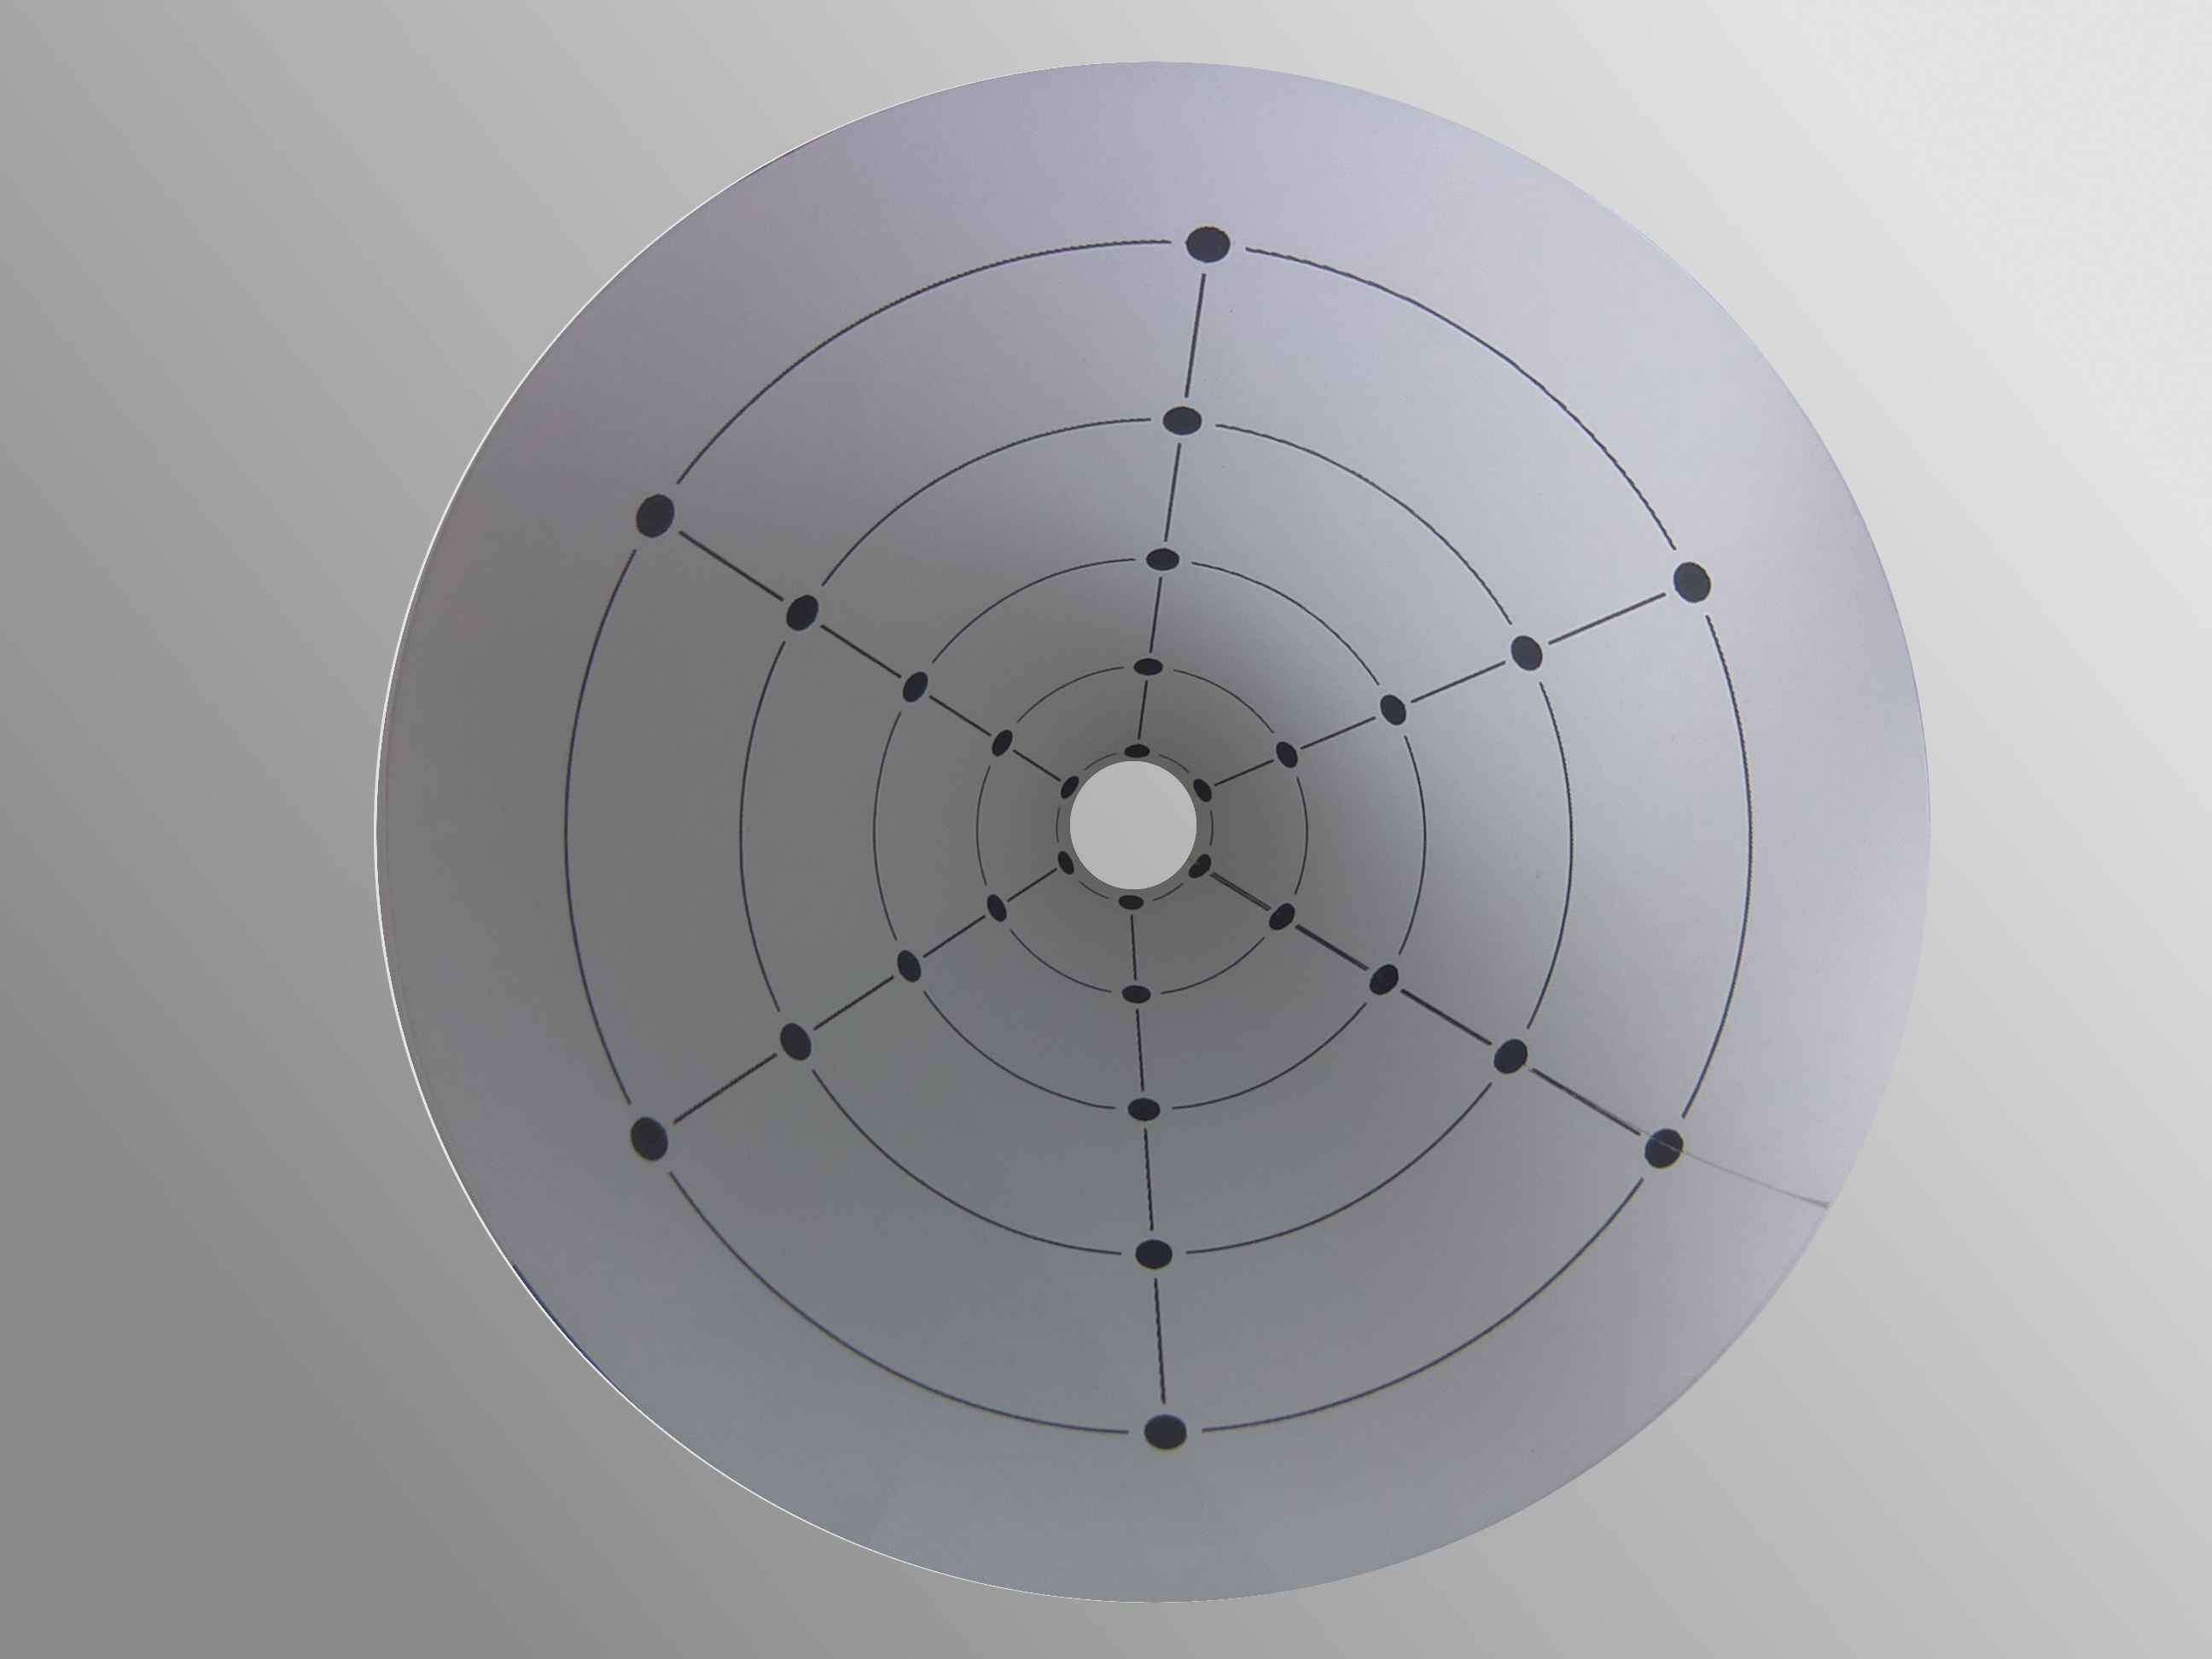
\includegraphics[width=.9\textwidth]{images/coneRasp.jpg}
		\caption{Ursprungsbild}
	\end{subfigure}%
	\begin{subfigure}{.5\textwidth}
		\centering
		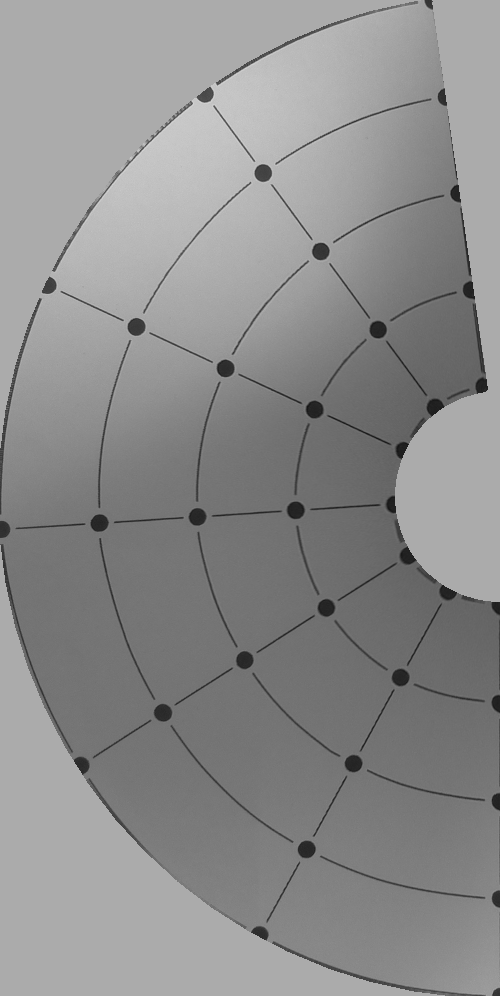
\includegraphics[angle=-90, width=.9\textwidth]{images/coneRaspUnWarpReverse.png}
		\caption{entfaltetes Bild (um 90° im Uhrzeigersinn gedreht)}
	\end{subfigure}
	\caption{Rückwärtsentfaltung}
	\label{fig:reverseUnfold}
\end{figure}

\cleardoubleoddemptypage
%!TEX root = bachelor.tex
\chapter{Implementierung}
\label{ch:implementation}

Zwecks Vereinfachung des Kalibrierungsprozesses wurde ein Assistent in Form einer graphischen Benutzerschnittstelle implementiert. 

Im ersten Schritt des Assistenten wird dabei optional, wie in Abbildung \ref{fig:wizard1} zu sehen, eine intrinsische Kamerakalibrierung durchgeführt. 
\begin{figure}[!htb]
	\centering
	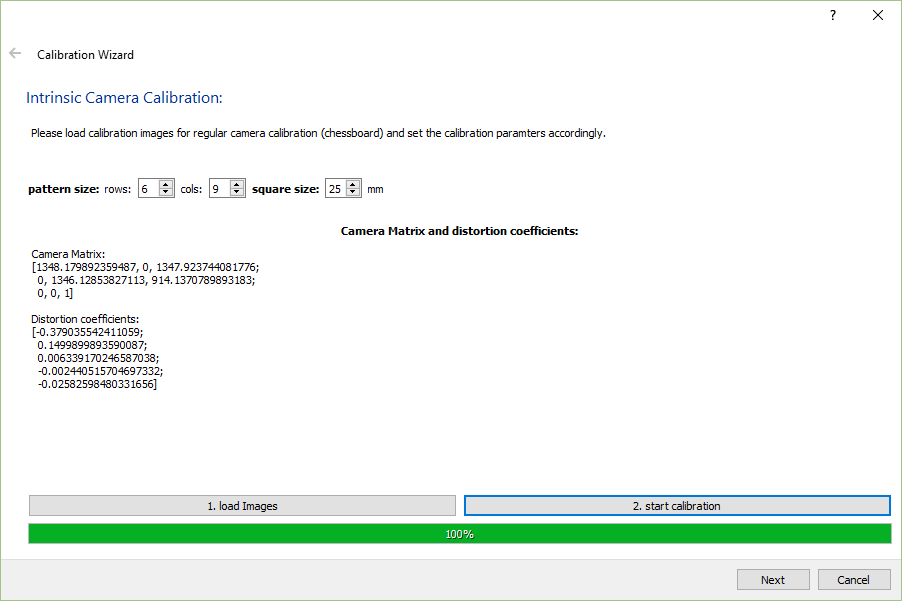
\includegraphics[width=0.9\textwidth]{images/GUI/calibWizard1_1.PNG}
	\caption{Kalibrierungsassistent: intrinsische Kamerakalibrierung}
	\label{fig:wizard1}
\end{figure}

Anschließend wird die eigentliche Kegelkalibrierung durchgeführt. Dabei wird zunächst das Kalibrierungsbild geladen und gegebenenfalls nach einer stattgefundenen intrinsischen Kalibrierung entzerrt. Es werden nun die Sample-Positionen detektiert und der Nutzer hat die Möglichkeit zu überprüfen, ob alle Positionen korrekt detektiert wurden und andernfalls fehlerhafte Punkte zu entfernen und / oder Punkte hinzuzufügen. Im Anschluss werden die Ellipsen und Liniensegmente bestimmt und Punktkorrespondenzen hergestellt (siehe Abbildung \ref{fig:wizard2}).

\begin{figure}[!htb]
	\centering
	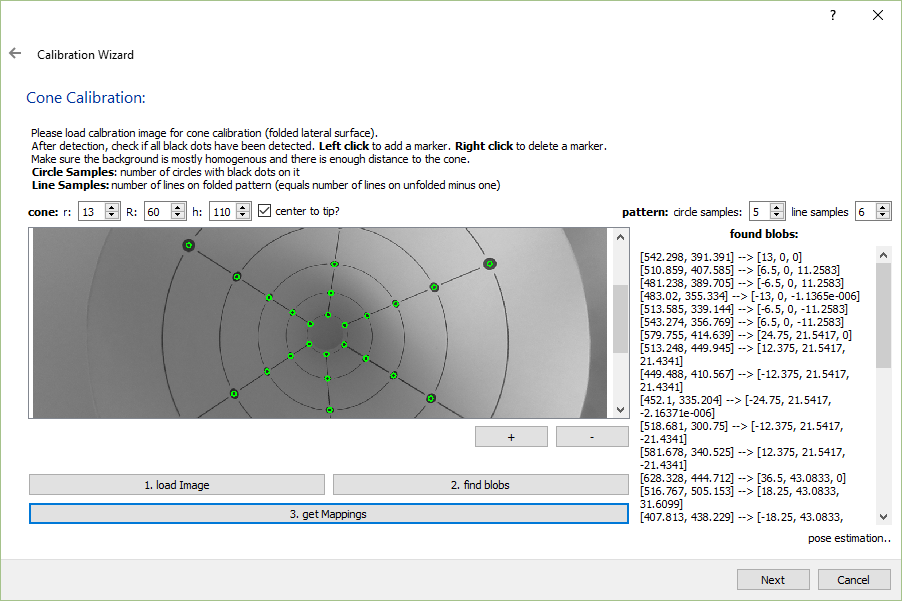
\includegraphics[width=0.9\textwidth]{images/GUI/calibWizard2_1.PNG}
	\caption{Kalibrierungsassistent: Kegelkalibrierung}
	\label{fig:wizard2}
\end{figure}

Im letzten Schritt kann zwischen beiden Entfaltungsverfahren gewählt werden. Anschließend können die Einstellungen in eine XML-Datei exportiert werden, in der, neben der Kamera-Matrix und Verzerrungskoeffizienten, auch die zwei Abbildungsmatrizen des ausgewählten Verfahrens gespeichert werden. 


Die Abbildungsmatrizen sind dabei wie folgt aufgebaut. Als $dst$ bezeichnen wir das entfaltete Bild. $src$ ist das Ursprungsbild.

Bei der Vowärtsentfaltung gilt:
\[
dst(map_x(x,y), map_y(x,y)) = src(x,y),
\]

wobei $map_x$ und $map_y$ die Abbildungsmatrizen sind und die gleiche Größe wie das Ursprungsbild haben. Für ein Pixel $(x,y)$ auf dem Ursprungsbild $src$ geben die Matrizen $map_x$, sowie $map_y$ an, auf welche Position ein das Pixel auf dem entzerrten Bild abgebildet wird. $map_x(x,y)$ bestimmt dabei die $x$-Koordinate, $map_y(x,y)$ die $y$-Koordinate. Da wir bei der Entfaltung die Größe des Ergebnisbildes benötigen, und wir diese bei der Erstellung der Abbildungsmatrizen berechnet haben, sind Breite und Höhe, in $map_x(0,0)$, respektive $map_y(0,0)$ kodiert. Für das Pixel an der Position $(0,0)$ auf dem Ursprungsbild ist anschließend keine Auswertung der Matrizen mehr möglich. Dieses Pixel ist jedoch ohnehin nicht Teil des Kalibrierungsmusters.

Bei der Rückwärtsentfaltung gilt:
\[
dst(x,y) = src((map_x(x,y),map_y(x,y)),
\]
wobei $map_x$ und $map_y$ wieder die Abbildungsmatrizen sind, die analog zur Vorwärtsenfaltung aufgebaut sind. Der grundlegende Unterschied ist hier, dass die wir von einem Pixel auf dem entzerrten Bild auf eine Position auf dem Ursprungsbild schließen. Die Abbildungsmatrizen haben hier die  gleiche Größe wie das entfaltete Bild. Eine Kodierung wie bei der Vowärtsentfaltung ist hier also nicht notwendig.

\cleardoubleoddemptypage
%!TEX root = bachelor.tex
\chapter{Analyse}
\label{ch:analysis}

Im folgenden Kapitel vergleichen wir beide in Kapitel \ref{ch:method} vorgestellten Verfahren zur Entzerrung. Anschließend gehen wir auf verschiedene Einflussfaktoren auf die Qualität und Präzision der Entzerrung ein, woraufhin wir die Laufzeiten analysieren. Im letzten Teil des Kapitels evaluieren wir beide Ansätze zur Ellipsendetektion.


Die Laufzeitanalysen wurden dabei auf einem \textbf{Raspberry Pi 2 Model B} mit folgenden Eigenschaften durchgeführt:
\begin{itemize}
	\item 900MHz quad-core ARM Cortex-A7 CPU
	\item 1GB RAM
	\item GCC-4.9.2
	\item Opencv 2.4.13
\end{itemize}


\section{Vergleich Vorwärtsentfaltung und Rückwärtsentfaltung}
Untersucht man die interpolierten Weltkoordinaten bei der Vorwärtsentfaltung, stellt man fest, dass die Oberfläche des Kegels,  wie in Abbildung \ref{fig:3DInterpol} zu sehen, eckig scheint. Zur Veranschaulichung wird hierbei nur ein Bruchteil der interpolierten Werte dargestellt. Zwischen den Samples auf einer Kreislinie sollten die interpolierte Positionen nach außen gewölbt sein, da ein Kegel rund ist. Da wir jedoch interpolieren und nicht extrapolieren, gehen die Werte nie über die zur Interpolation genutzten Werte hinaus. Konkreter kann eine interpolierte Position keine größeren oder kleineren $x$- und $y$-Koordinaten erhalten, als die der genutzten Samples. Diese wäre jedoch notwendig, sodass die Rundung des Kegels erhalten bleibt.

\begin{figure}[!htb]
	\centering
	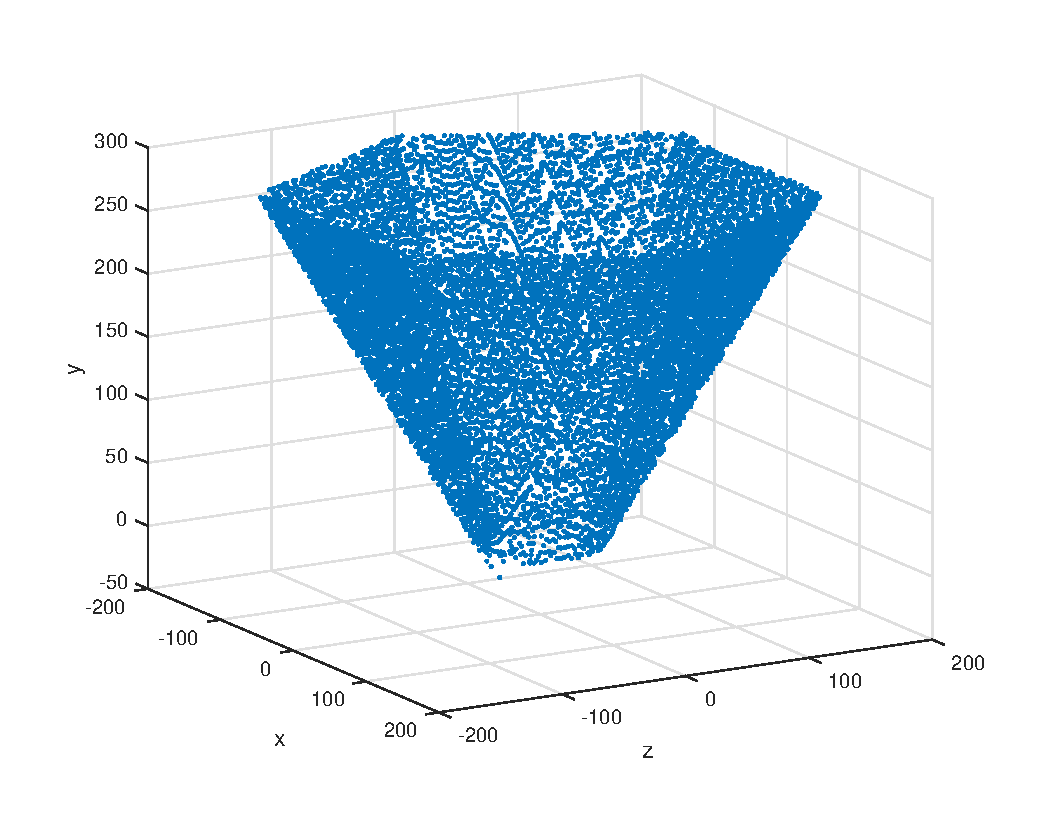
\includegraphics[scale=.7]{images/3d_interpol.eps}
	\caption{interpolierter Kegel}
	\label{fig:3DInterpol}
\end{figure}

\begin{figure}[!htb]
	\centering
	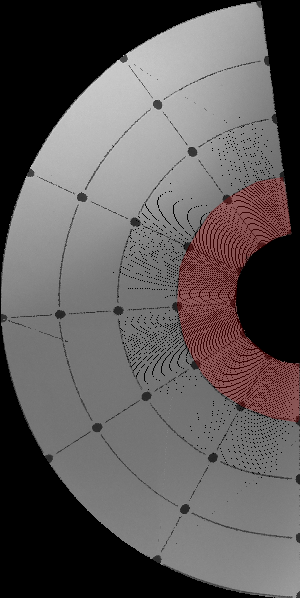
\includegraphics[angle=-90, width=.7\textwidth]{images/coneRaspUnWarpForwardHigh.png}
	\caption{Vorwärtsentfaltung}
	\label{fig:forwardHoles}
\end{figure}

Darüber hinaus zeigt sich ein weiteres Problem nach der Entfaltung. Die Entfaltung geschieht über die Abbildung \ref{eq:coneToLateral}, die in Kapitel \ref{s:cone} konstruiert wurde.
Damit im entfalteten Bild nicht 1mm einem Pixel entspricht, müssen die erhaltenen Werte skaliert werden. Wir wollen dabei entsprechend einer gewünschten Auflösung der entzerrten Seitenhöhe skalieren.
Auch schon bei kleineren Skalierungen entstehen auffällige Risse im entfalteten Bild, die in Abbildung \ref{fig:forwardHoles} exemplarisch zu sehen sind. Grund dafür ist, dass jedes Pixel aus dem Ursprungsbild auf eine 2D-Koordinate der Mantelfläche abgebildet wird. Auch nach einer Skalierung handelt es sich bei diesen Werten im Allgemeinen nicht um ganzzahlige Werte. Es entstehen Rundungsfehler. Auch wenn Rundungsfehler nicht entständen, fehlte es auf Grund der starken Stauchung, in den inneren, kleineren Regionen (siehe Abbildung \ref{fig:forwardHoles} in rot) des Ursprungsbild an genügend Bildinformation. Solche Risse, beziehungsweise nicht erreichte Pixel auf dem entfalteten Bild, bezeichnen wir als Defekte.

Da wir von dem Ursprungsbild aus auf das entfaltete Bild abbilden, ist außerdem eine Interpolation auf dem Ursprungsbild nicht möglich, da wir vorher nicht wissen, wo Defekte entstehen. Man müsste also entweder auf dem resultierendem Bild interpolieren (siehe Kapitel \ref{ch:summary}), oder zu gegebenen Defekten über die Umkehrabbildung auf Pixelkandidaten im Ursprungsbild schließend und dann entsprechend interpolieren.
Es bietet sich dann jedoch an, direkt die Umkehrabbildung zu nutzen, was die Motivation hinter der Rückwärtsentfaltung ist.

Wir möchten untersuchen wie sich die Anzahl der Defekte bei einer Änderung der Ausgabeauflösung der Seitenhöhe verhält. Diese Beziehung lässt sich in Abbildung \ref{fig:influenceRes} ablesen.
\begin{figure}[!htb]
	\centering
	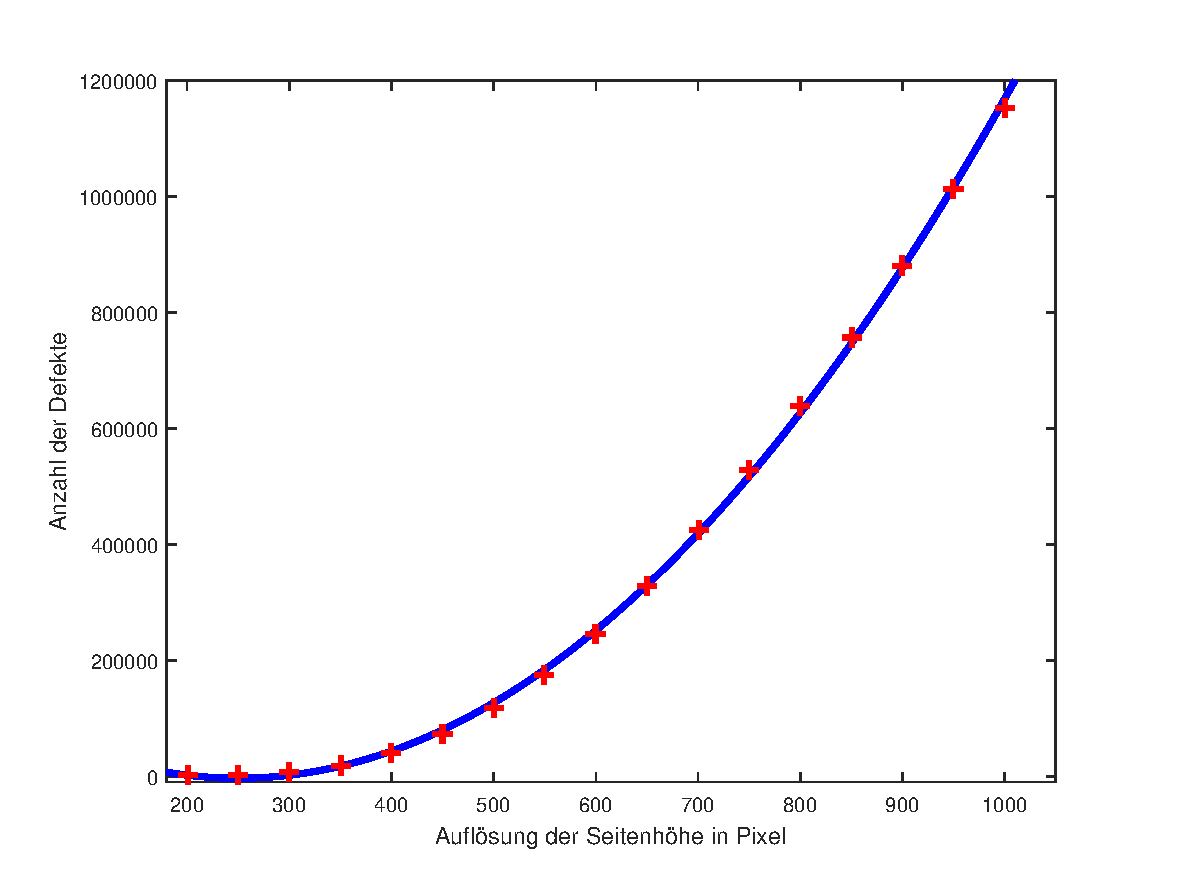
\includegraphics[width=\textwidth]{images/numberOfHoles.eps}
	\caption{Einfluss der Ausgabeauflösung auf die Anzahl der Defekte}
	\label{fig:influenceRes}
\end{figure}

Wie erwartet verhält sich die Anzahl der Defekte quadratisch zur gewählten Ausgabeaufösung. Der Informationsgehalt (Pixelanzahl) des Ursprungsbild bleibt trotz erhöhter Ausgabeauflösung konstant. Wie in Abbildung \ref{fig:sizeOutput} zu sehen, verhält sich die Ausgabeauflösung $res_S$ quadratisch zur Gesamtzahl der Pixel für ein konstantes $\alpha$. Für die Breite $b$ des Ausgabebildes gilt $b = res_S$.
Die Höhe $h$ setzt sich wie folgt zusammen: $h = res_S + res_S\cdot\cos(2\pi-\alpha) = res_S\cdot(1 + cos(2\pi-\alpha)) = res_S\cdot(1+\cos\alpha)$. Dazu betrachten wir das rechtwinklige Dreieck in der rechten oberen Ecke der Abbildung (in magenta). Die Hypotenuse des Dreiecks beträgt $res_S$ und mit $\beta = 2\pi - \alpha$ ergibt sich für die Ankathete eine Länge von $res_S\cdot\cos(2\pi-\alpha)$. Die Gesamtzahl der Pixel beträgt demnach $b\cdot h = res_S^2(1+\cos(\alpha))$.

\begin{figure}[!htb]
	\centering
	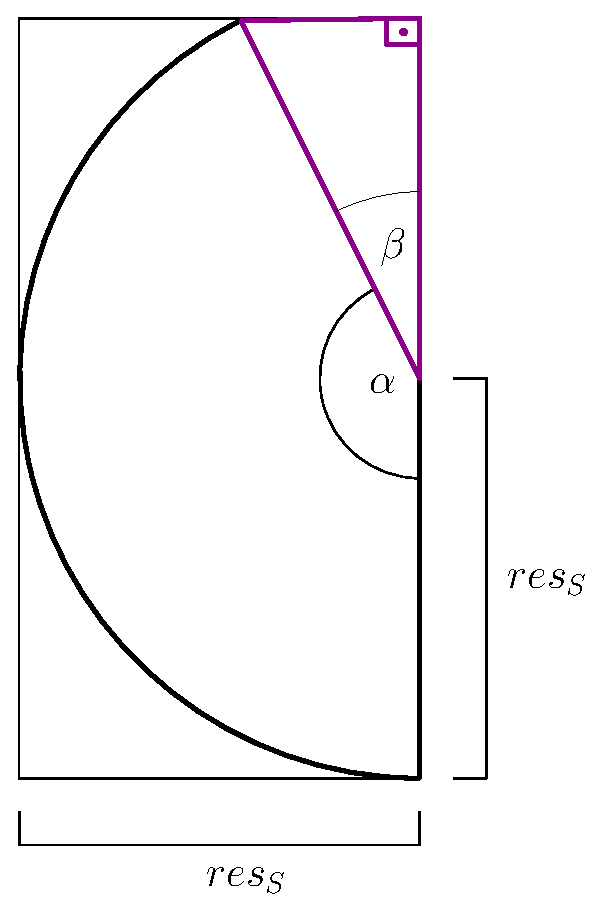
\includegraphics[width=0.3\textwidth]{images/sizeOutput.eps}
	\caption{Größe des Ausgabebildes bei einer Seitenhöhe von $res_S$}
	\label{fig:sizeOutput}
\end{figure}


Obwohl die Laufzeit der Kalibrierung nicht im Vordergrund steht, vergleichen wir die Laufzeit beider Verfahren bei verschiedenen Auflösungen der Seitenhöhe. Da der Großteil des Kalibrierungsprozesses bei beiden Verfahren identisch ist, vergleichen wir nun den Teil, der sich unterscheidet. Das heißt wir messen bei der Vorwärtsentfaltung die Laufzeit für die Interpolation der Weltkoordinaten und die anschließende Abbildung auf die Mantelfläche, und bei der Rückwärtsentfaltung die Laufzeit für die Abbildung auf die Kegelkoordinaten, die Bestimmung der Projektionsmatrix und die anschließende Abbildung auf die Bildkoordinaten, inklusive Interpolation.


Wie in Abbildung \ref{fig:runningTimeComparision} zu sehen, ist der Aufwand bei bei der Vorwärtsentfaltung weitestgehend konstant. Dies da dadurch zu begründen, dass sich die Eingabeauflösung nicht ändert. Der Interpolationsaufwand bleibt gleich und es wird anschließend die gleiche Anzahl Pixel auf die Mantelfläche abgebildet. Nur der Ort der Projektion wird entsprechend der Ausgabeauflösung skaliert.
Bei der Rückwärtsentfaltung hingegen, wächst der Interpolationsaufwand quadratisch. Wir gehen dort von dem Ausgabebild aus, das quadratisch mit der Auflösung wächst und bilden dort jeden Punkt auf das Ursprungsbild ab. Je mehr Pixel auf dem Ausgabebild, desto häufiger muss interpoliert werden. Bei einer Auflösung der Seitenhöhe von $850$ Pixeln ist die Laufzeit bei beiden Verfahren gleich.

\begin{figure}[!htb]
	\centering
	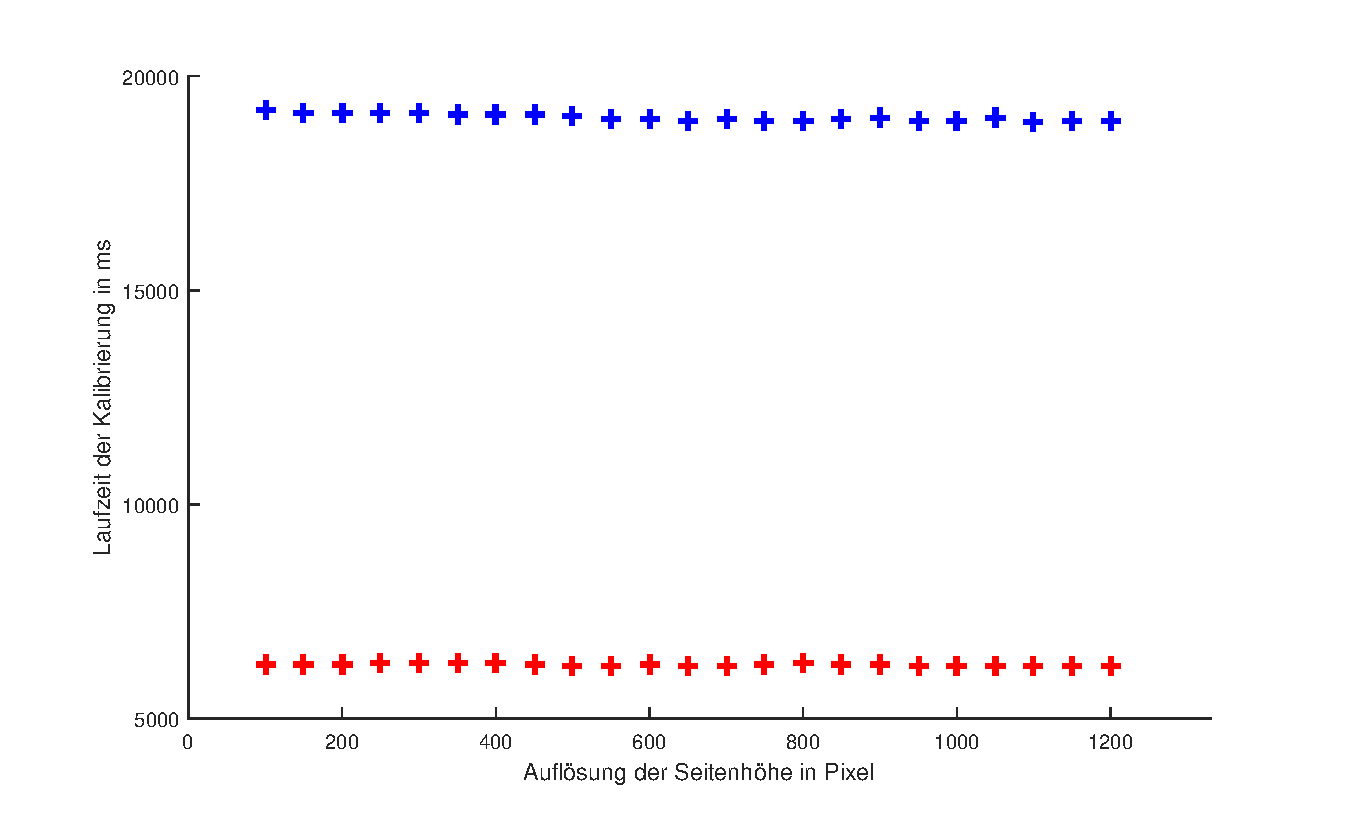
\includegraphics[width=0.9\textwidth]{images/runningTimeCalibration.eps}
	\caption{Laufzeitvergleich zwischen Vorwärtsentfaltung (blau) und Rückwärtsentfaltung (rot)}
	\label{fig:runningTimeComparision}
\end{figure}


\bigskip

Als Reprojektionsfehler einer Abbildung wird die Distanz zwischen einem gemessenem Punkt und einem korrespondierendem (durch die Abbildung) projizierten Punkt bezeichnet.


Im Falle der Rückwärtsentfaltung sind die gemessenen Punkte die Bildpositionen der Samples im Ursprungsbild. Da die Geometrie des Kegels bekannt ist, wissen wir wo sich die  Samples auf dem entfalteten Bild befinden müssen (siehe Parametrisierung der Mantelfläche \ref{eq:paramLateral} in Kapitel \ref{ch:theory}). Wir können nun diese Positionen mit Hilfe der Abbildung zur Entfaltung und der Projektionsmatrix zurück auf das Ursprungsbild abbilden. Diese Punkte sind die projizierten Punkte. Da die Abbildung von der Mantelfläche zur Kegeloberfläche exakt ist, ist der Reprojektionsfehler der Rückwärtsentfaltung alleine durch die Projektionsmatrix bestimmt.

Bei der Vorwärtsentfaltung sind die gemessenen Punkte gegeben durch die bekannten Sample-Positionen auf der Mantelfläche. Die projizierten Punkte erhält man, nach der Abbildung der detektierten Sample-Positionen des Ursprungsbild auf die Mantelfläche. Der Reprojektionsfehler ist also alleine durch die Genaugkeit der Sample-Detektion definiert und somit bei diesem Verfahren immer nahe null.
Obwohl das Endergebnis, bedingt durch die Defekte, bei der Vorwärtsentfaltung optisch schlechter ist, ist der Reprojektionsfehler also bei der Vorwärtsentfaltung im Allgemeinen kleiner.
Als Vergleich zwischen den beiden Verfahren eignet sich der Reprojektionsfehler demnach nicht.

Auf Grund der fehlenden Defekte bei der Rückwärtsentfaltung und der besseren Laufzeit bei Auflösungen unter 850 Pixeln, beziehen sich alle folgenden Auswertungen nur noch auf die Rückwärtsentfaltung.


\section{Einfluss der intrinsischen Kalibrierung}
Ein wichtiger Einflussfaktor auf die Qualität der Entzerrung ist die intrinsische Kamerakalibrierung, die vor der eigentlichen Kegelkalibrierung stattfindet. Ihre Hauptaufgabe besteht darin, die Linsenverzerrungen der Kamera herauszurechnen.

Wir messen den Einfluss der Kamerakalibrierung mit Hilfe des Reprojektionsfehlers. Dazu betrachten wir fünf verschiedene Bilder, die ein Mal mit und ein Mal ohne intrinsische Kalibrierung entzerrt werden. Bei beiden Gruppen wird anschließend jeweils der Reprojektionsfehler pro Sample bestimmt und verglichen. Die Ergebnisse sind in Abbildung \ref{fig:influenceCalib} zu sehen. In der linken Abbildung sind hierbei die Fehler im kalibrierten Fall zu sehen, im Linken im unkalibrierten Fall. In der Abbildung ist dabei ein Kreuz an der Stelle $(u,v)$, falls die Abweichung des projizierten Punktes in $x$-Richtung $u$, sowie in $y$-Richtung $v$ beträgt.

\begin{figure}[!htb]
	\centering
	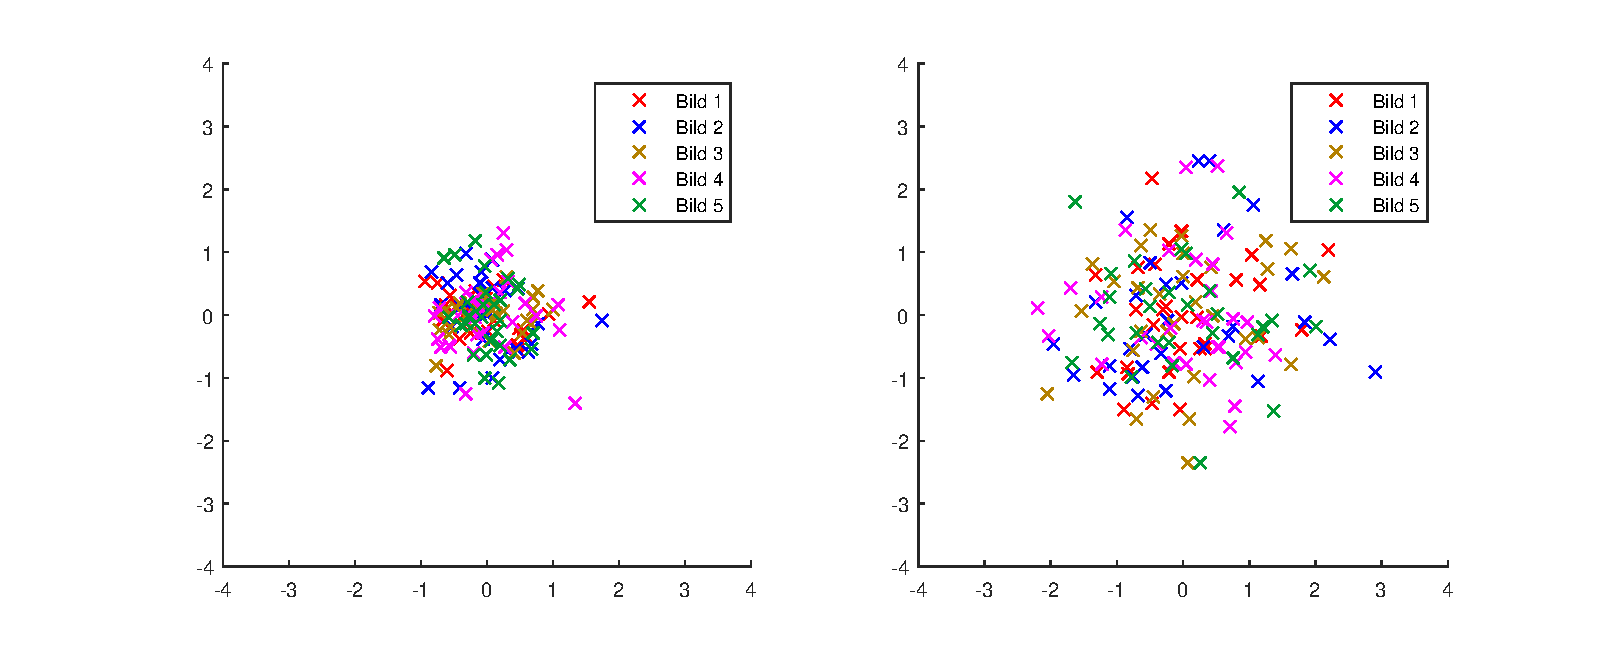
\includegraphics[width=\textwidth]{images/reprojectionErrorReverse.eps}
	\caption{Einfluss der intrinsischen Kalibrierung auf den Reprojektionsfehler}
	\label{fig:influenceCalib}
\end{figure}


Es ist klar zu erkennen, dass der Reprojektionsfehler bei den Bildern ohne intrinsische Kamerakalibrierung wesentlich größer ist. Der starke Einfluss kommt unter Anderem daher, dass wir eine Weitwinkelkamera mit starker tonnenförmiger Verzerrung eingesetzt haben. Ohne eine Modellierung der Linsenverzerrungen weichen die Abstände zwischen den Sample-Positionen stark von der Realität ab. Die Projektionsmatrix wird mit fehlerhaften Daten bestimmt. Die eigentlichen Sample-Positionen auf dem entzerrten Bild, werden also nicht korrekt auf die Sample-Positionen im Ursprungsbild abgebildet.

\section{Einfluss der Rotation der Kamera}
Um den Einfluss der Rotation der Kamera untersuchen zu können, wurde der Kegel mit Kalibrierungsmuster gerendert, da die Kameraposition dann exakt bekannt ist und äußere Faktoren wie Lichtverhältnisse und inhomogene Hintergründe kontrolliert werden können. In Abbildung \ref{fig:blender} ist bei zwei unterschiedlichen Winkeln der gerenderte Kegel zu sehen.

\begin{figure}[!htb]
	\centering
	\begin{subfigure}{.5\textwidth}
		\centering
		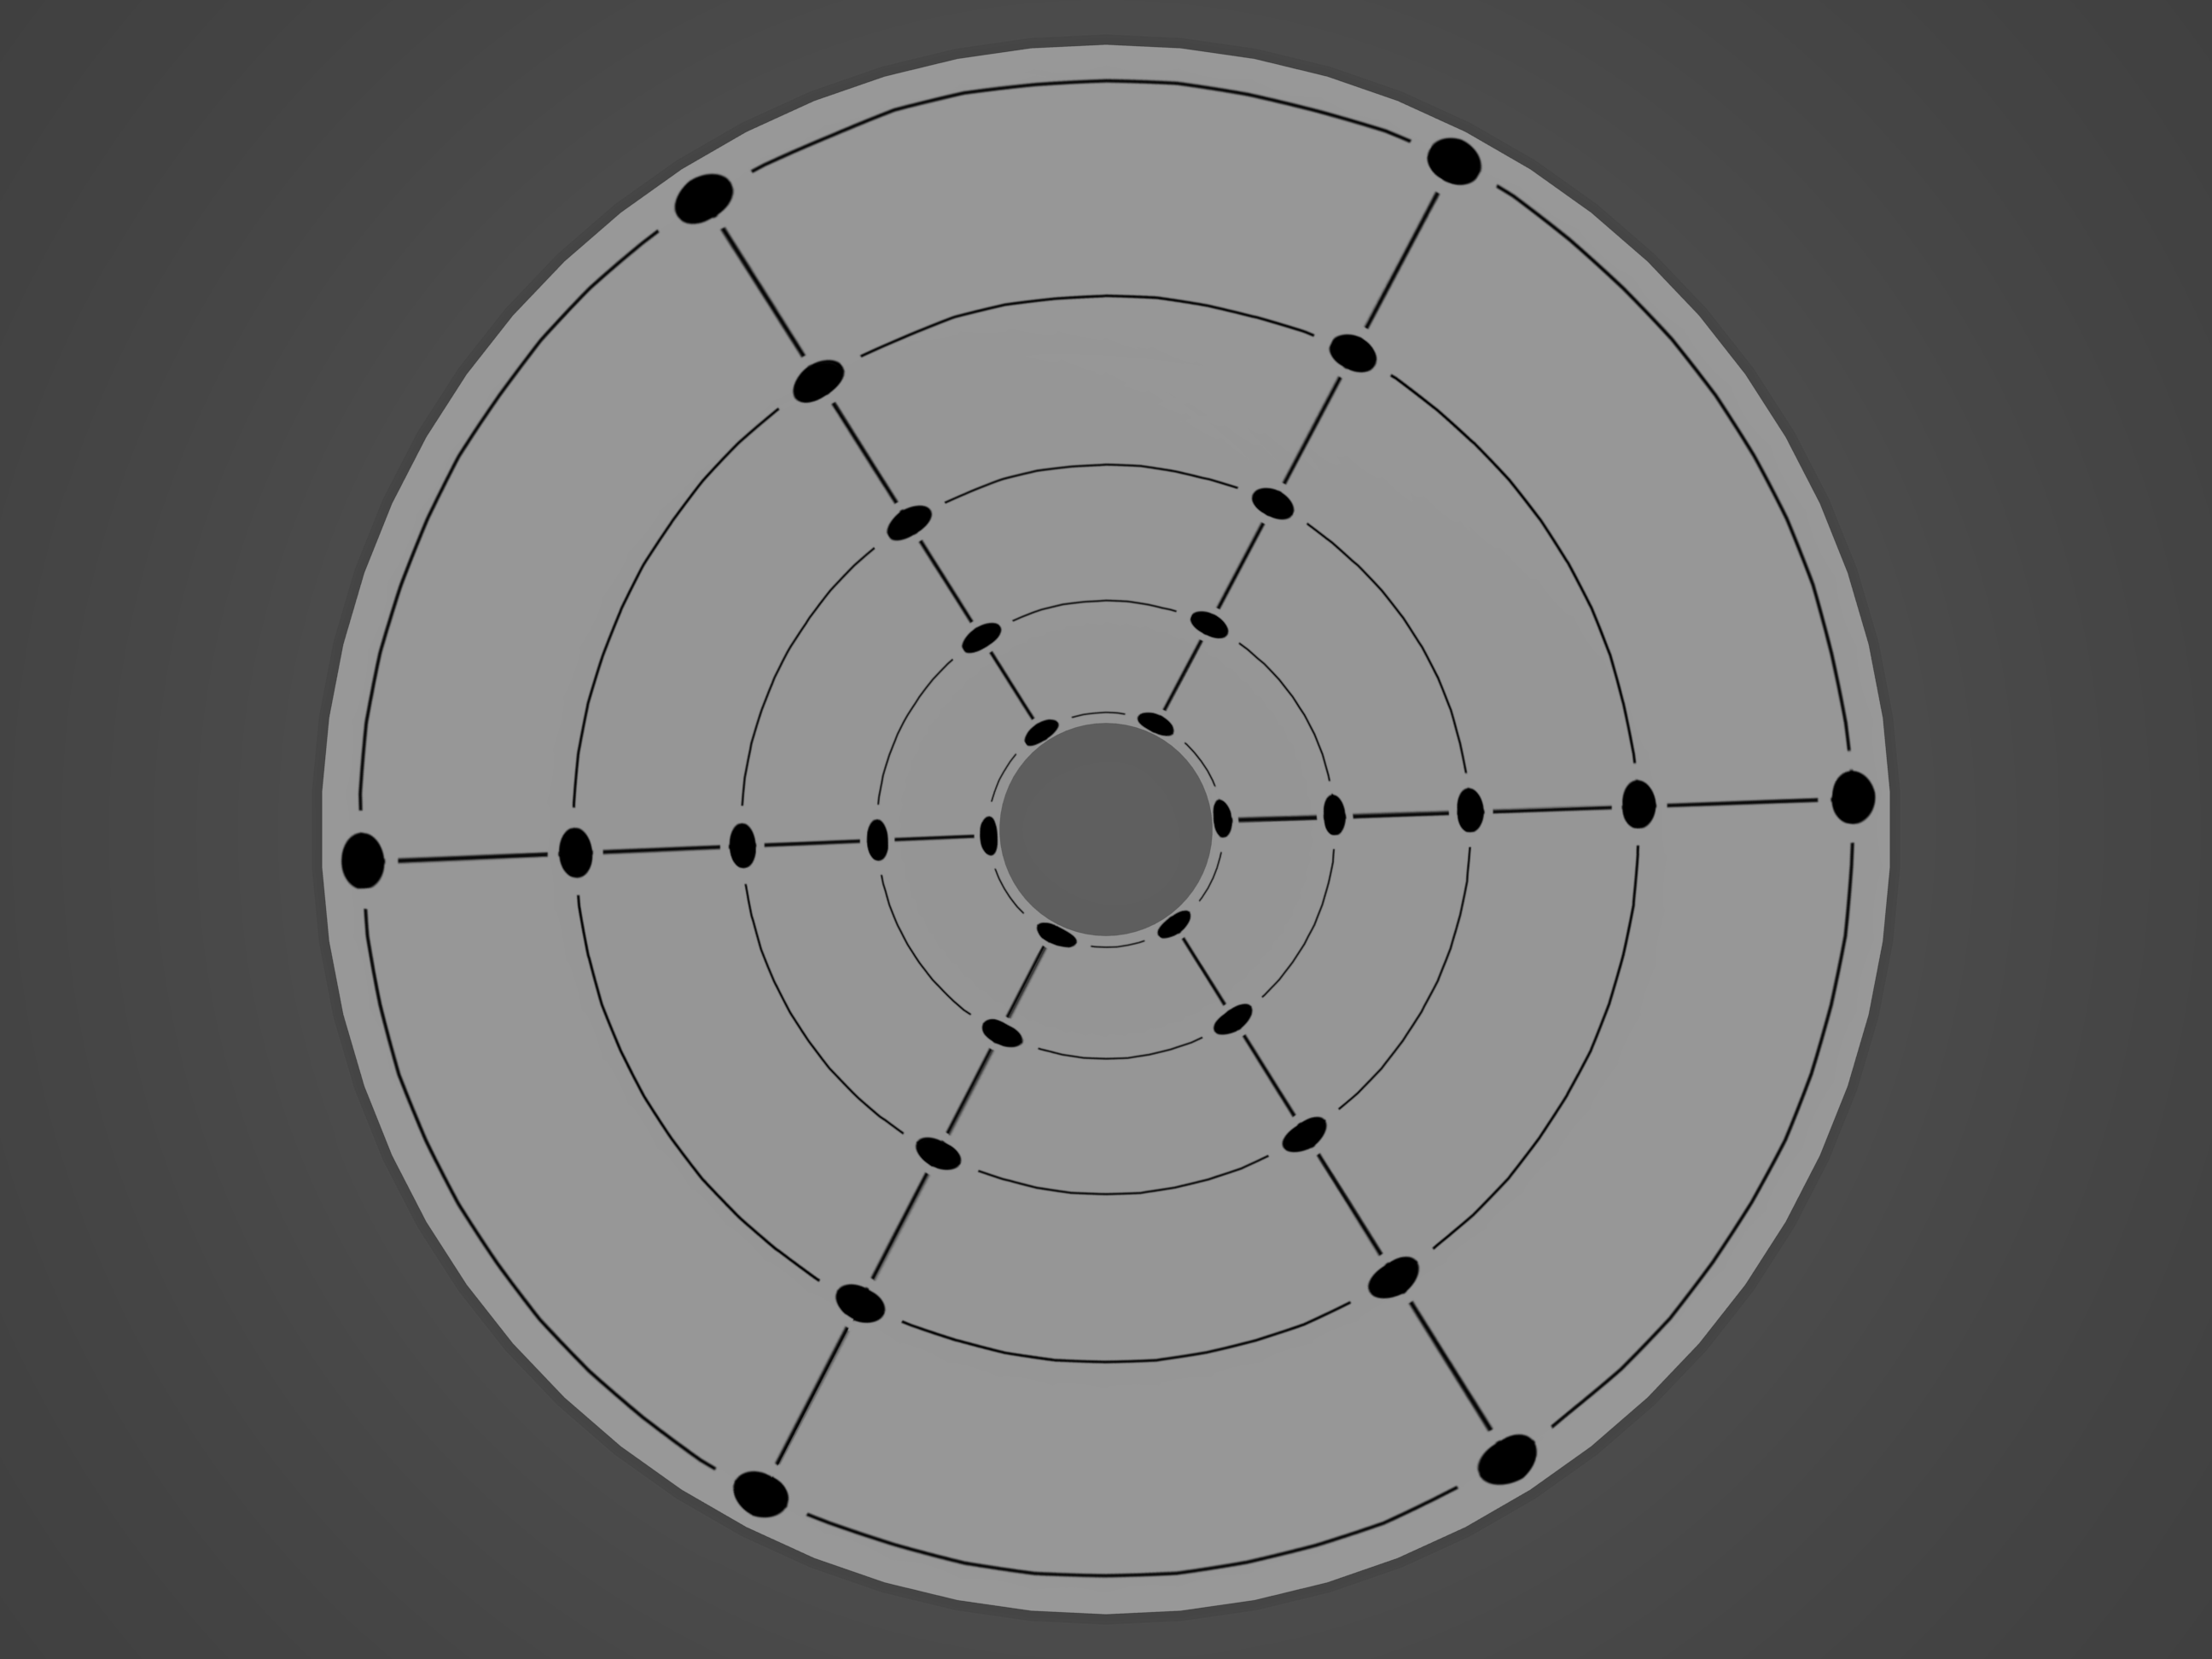
\includegraphics[width=.9\textwidth]{images/blender0.png}
		\caption{bei 0°}
	\end{subfigure}%
	\begin{subfigure}{.5\textwidth}
		\centering
		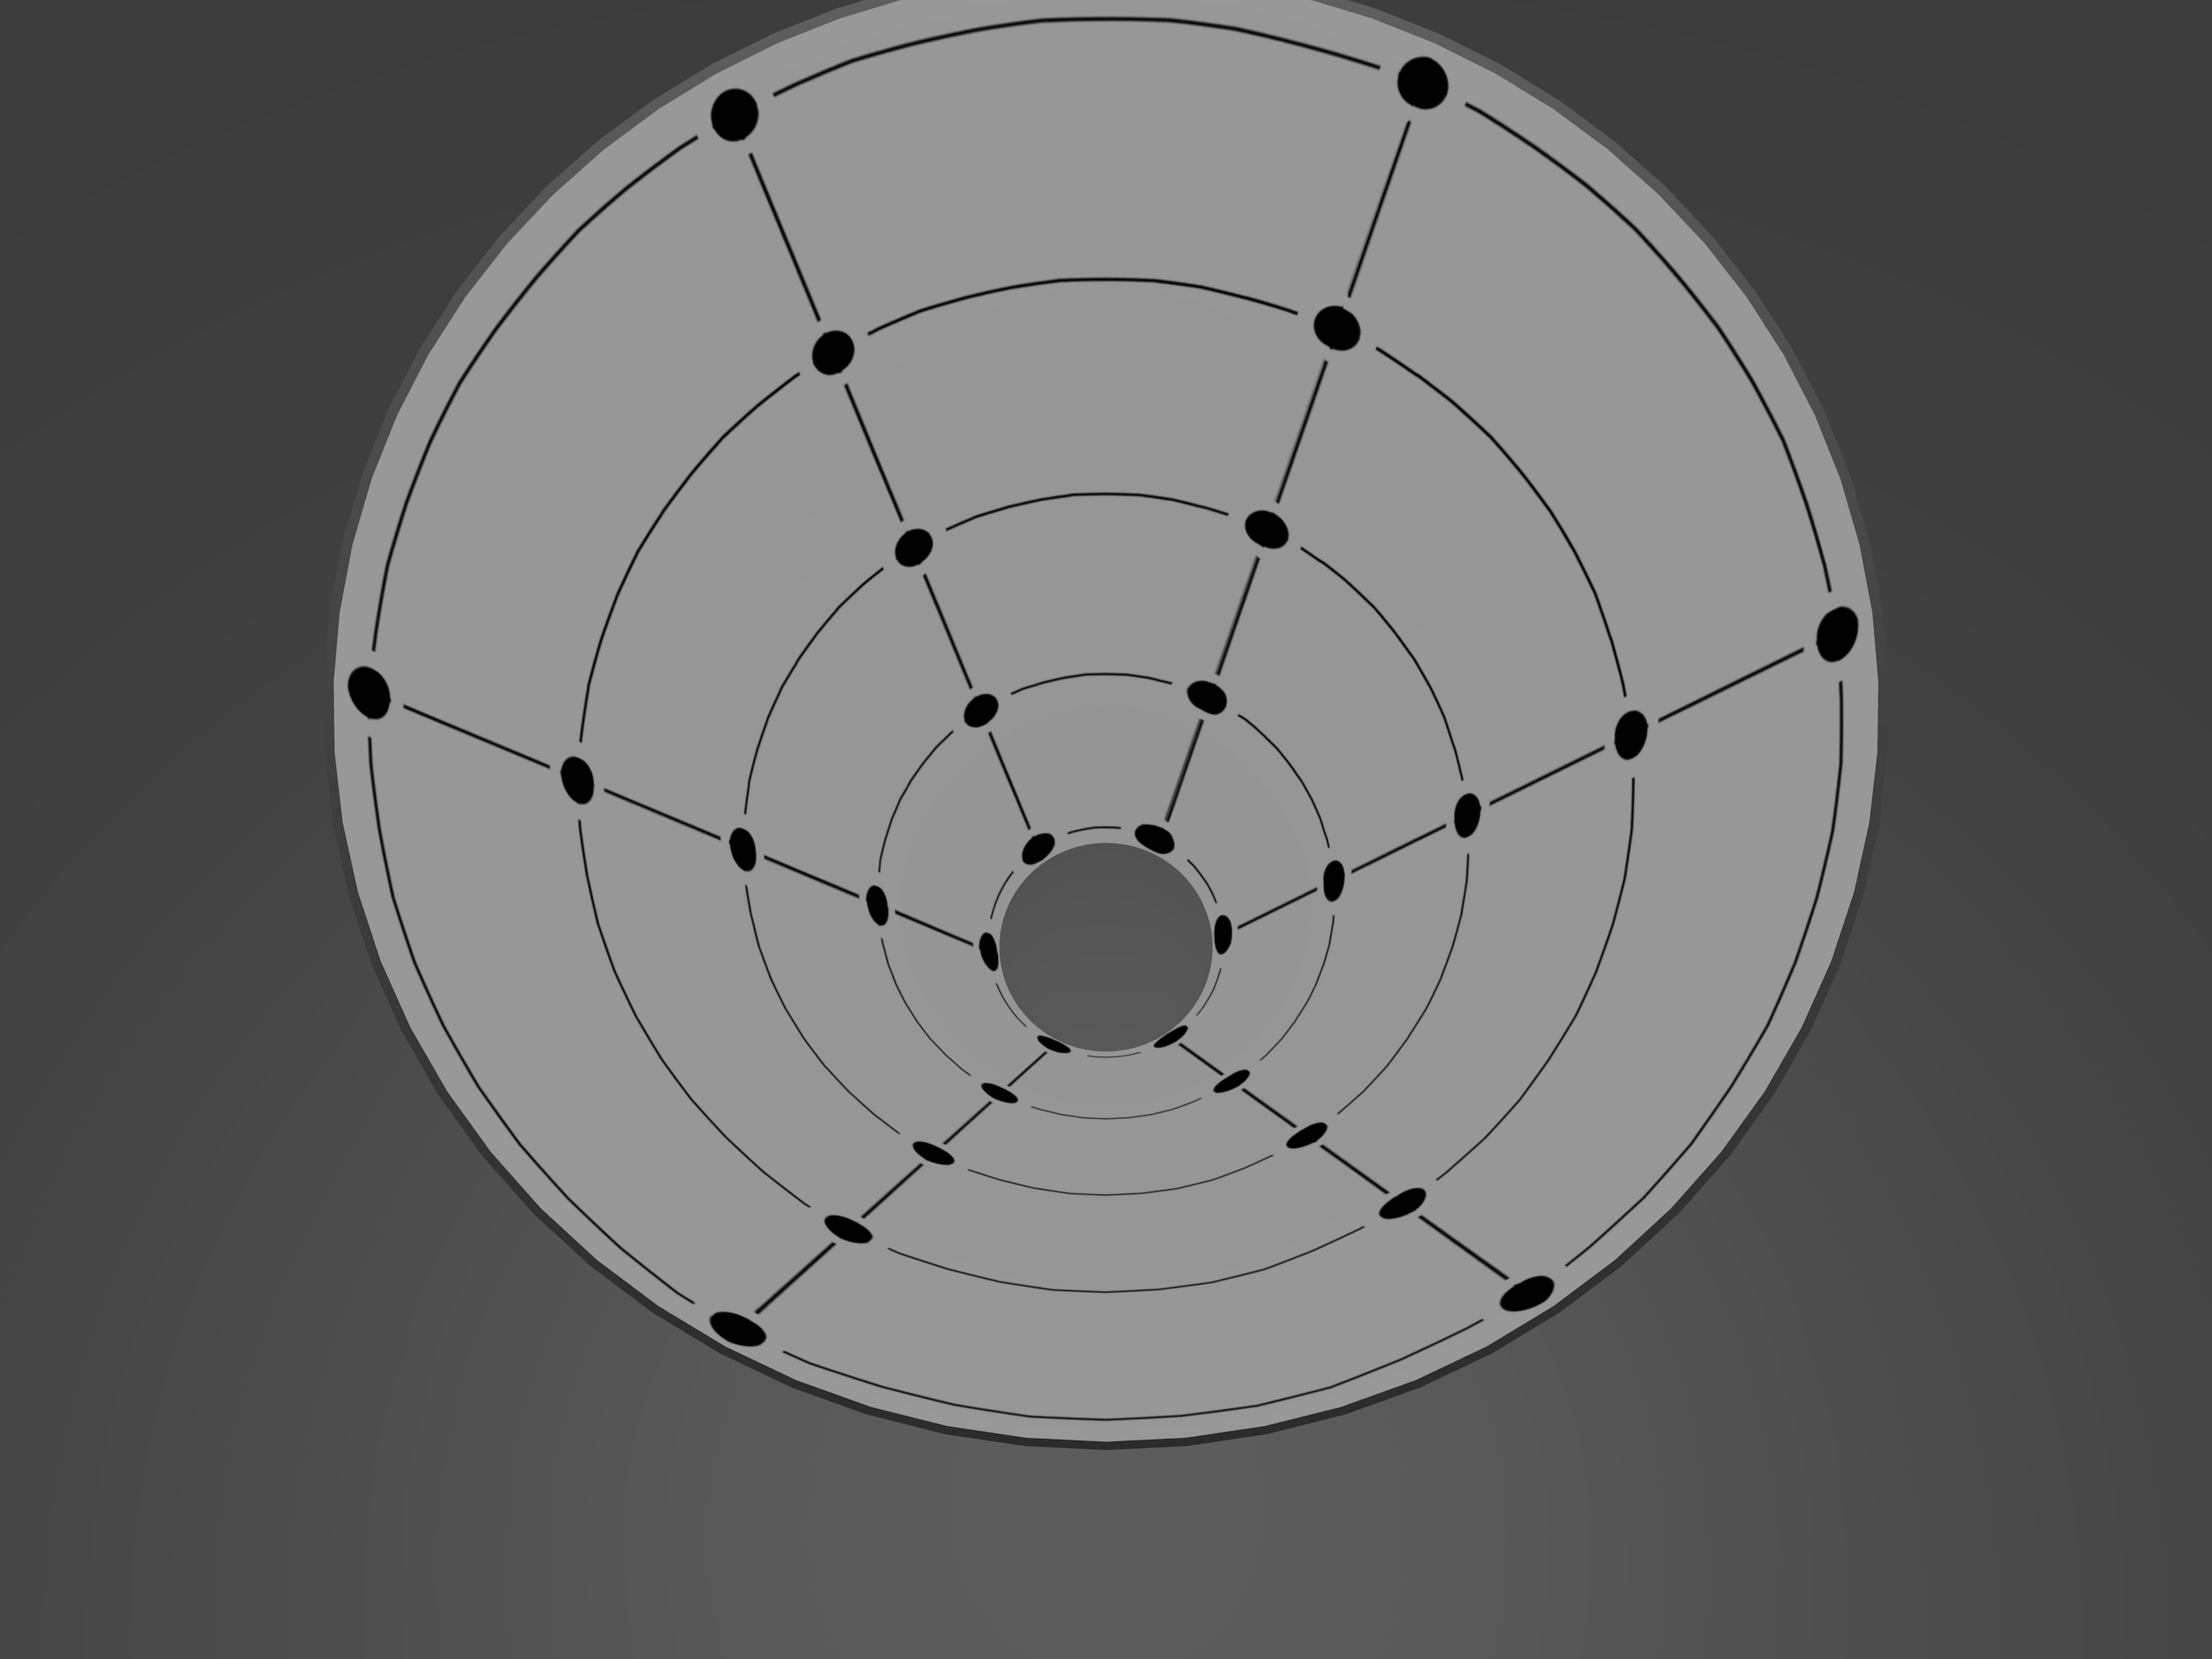
\includegraphics[width=.9\textwidth]{images/blender12.png}
		\caption{bei 12°}
	\end{subfigure}
	\caption{gerendeter Kegel mit Kalibrierungsmuster aus verschiedenen Blickrichtungen}
	\label{fig:blender}
\end{figure}


Es werden anschließend Bilder erzeugt, in denen in 1° Schritten die Kamera von 0° bis 16° um die $x$-Achse rotiert wird. Für jedes dieser Bilder wird anschließend eine Rückwärtsentfaltung durchgeführt und der durchschnittliche Reprojektionsfehler ermittelt. Abbildung \ref{fig:influenceRot} zeigt, dass der Reprojektionsfehler relativ rotationsinvariant ist bei einem durchschnittlichen Reprojektionsfehler von $1.925$. Ab einem Winkel von  13°, werden die Samples teilweise vom Blob-Detektor nicht mehr erkannt (bei 13° und 14° werden zwei nicht erkannt, bei 15° und 16° jeweiles vier) und mussten per Hand markiert werden. Ab einem Winkel von 16° sind die Abstände zischen den Kreislinien so klein, dass die Ellipsendetektion fehlschlägt.


\begin{figure}[!htb]
	\centering
	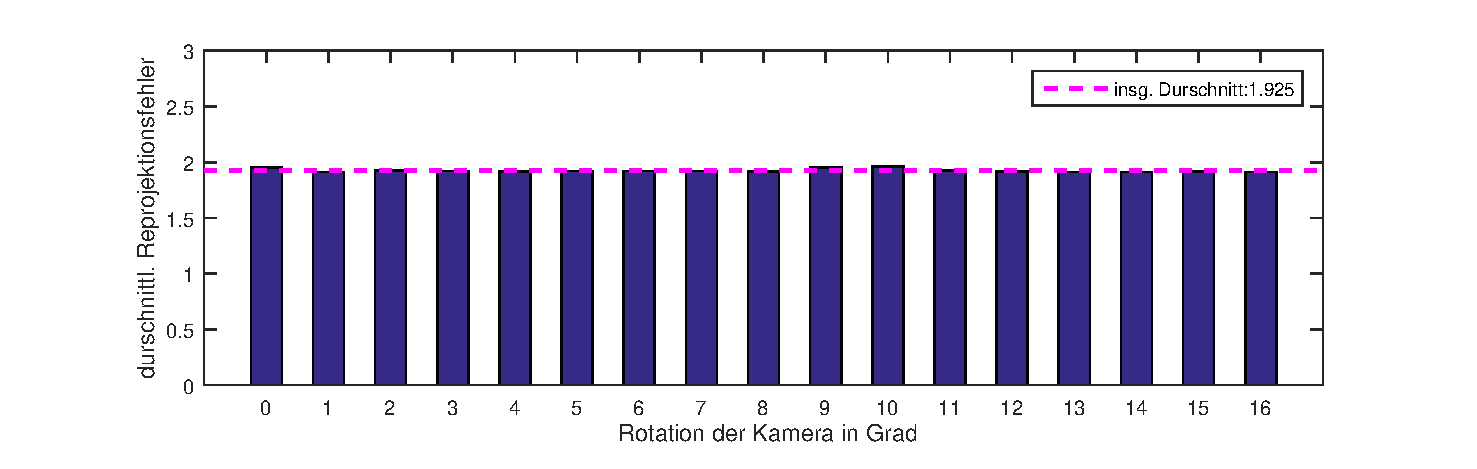
\includegraphics[width=\textwidth]{images/reprojectionErrorDeg2.eps}
	\caption{Einfluss der Rotation der Kamera}
	\label{fig:influenceRot}
\end{figure}


\section{Laufzeit der Entfaltung}
Durch den Kalibrierungsprozess erhalten wir zwei Abbildungsmatrizen (siehe Kapitel \ref{ch:implementation}), mit denen wir anschließend eine Reihe von Bildern entzerren möchten. Wir untersuchen dabei die Laufzeit pro gewählter Auflösung in 50er Schritten, und ermitteln jeweils die Laufzeit gemittelt über 200 Bilder. Untersucht wird die Laufzeit mit bikubischer, sowie mit (bi-) linearer Interpolation.

Im Gegensatz zu linearer Interpolation, werden bei bikubischer Interpolation 16 Nachbarn statt vier betrachtet und mittels (stückweise stetiger) Polynome interpoliert. Der Aufwand bei der bikubischen Interpolation ist wesentlich größer, es entstehen aber weniger Artefakte \cite{Keys1981}.

Wie in Abbildung \ref{fig:influenceRes2} zu sehen, wächst die Laufzeit bei beiden Verfahren quadratisch mit der Auflösung der Seitenhöhe. Die Laufzeit des Verfahrens mittels bikubischer Interpolation wächst dabei um einen Faktor von circa $1.35$ schneller, als das Verfahren mittels linearer Interpolation.

\begin{figure}[!htb]
	\centering
	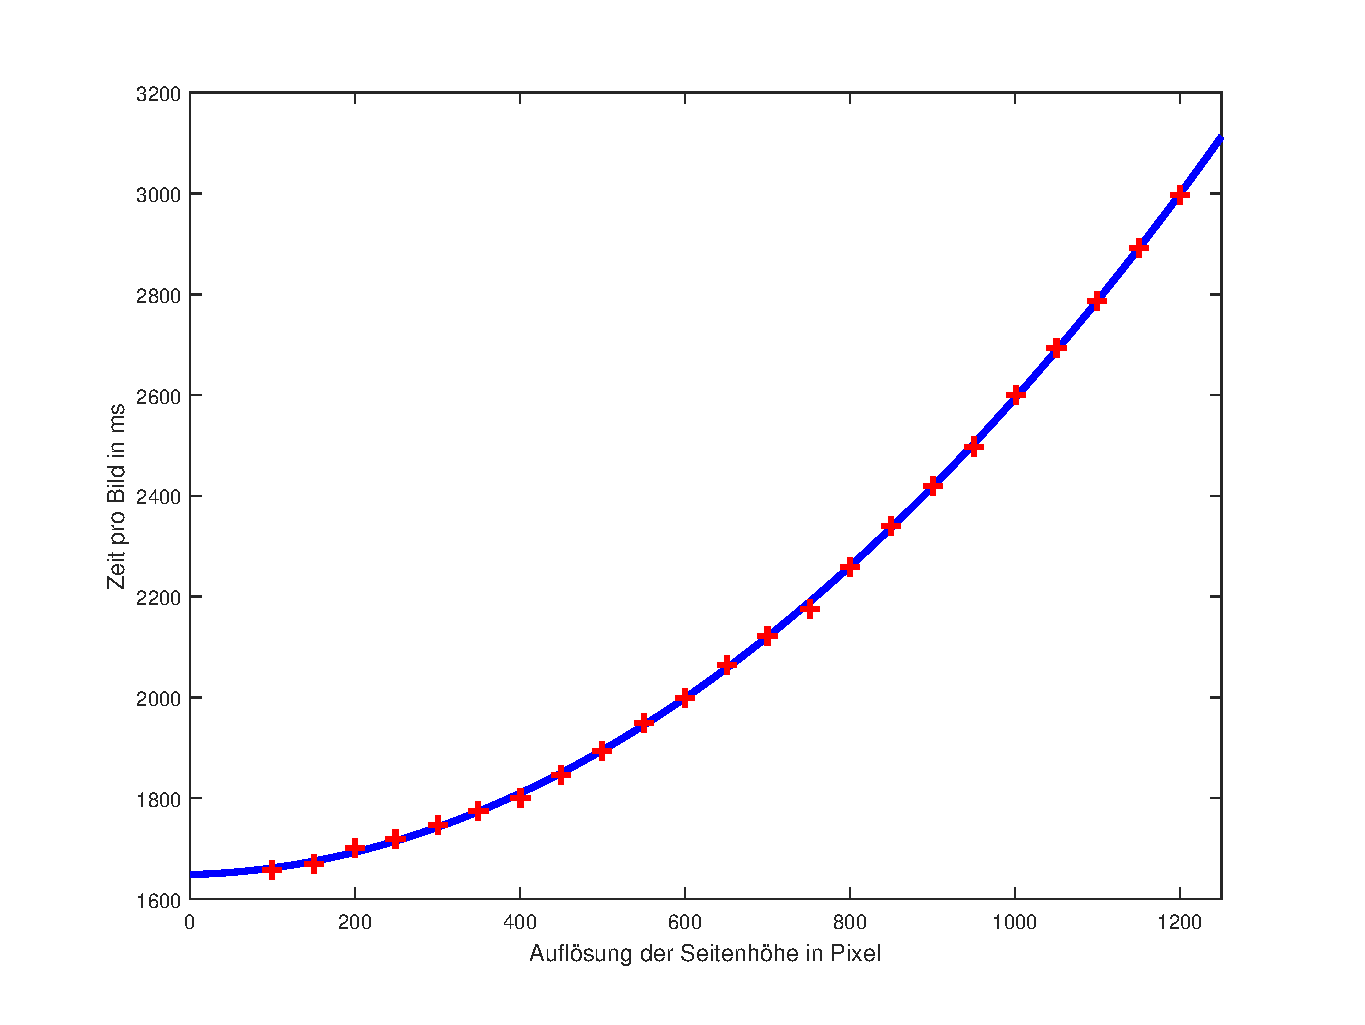
\includegraphics[width=0.8\textwidth]{images/runningTimePerSlantheight.eps}
	\caption{Einfluss der Ausgabeauflösung auf die Laufzeit der Entfaltung}
	\label{fig:influenceRes2}
\end{figure}

\section{Evaluierung der Ellipsendetektion mittels Deformable Templates}
Das Problem bei der Ellipsendetektion mittels {Deformable Templates ist, dass die Energiefunktion, auch nach starker Glättung des Kanten- und Kantenrichtungsbilds, schnell in kleine lokale Minima läuft, obwohl ein wesentlich stärkeres Minimum in näherer Umgebung wäre.

In Abbildung \ref{fig:deformable} sieht man beispielhaft einen Auschnitt der Energiefunktion, wobei in diesem Fall zwecks Veranschaulichung nur die Haupt- und Nebenachse der Ellipse variable sind. Das Zentrum bleibt das Zentrum des Bildes und der Winkel $\theta$ ist konstant null. Trotz dieser Einschränkungen lässt sich gut erkennen, dass circa bei $a = b = 350$ ein starkes Minimum liegt. Es gibt jedoch neben diesem Minimum in näherer Umgebung kleine irrelevante Minima, wie beispielsweise in $(350, 260)$. Solche "`Becken"' (in rot markiert) erschweren die Detektion erheblich.

Darüber hinaus muss für ein robustes und effizientes Optimierungsverfahren der Gradient und im besten Fall sogar die Hesse-Matrix der zu minimierenden Funktion zur Verfügung gestellt werden.  Jede Ableitung des Kanten- und Kantenorientierungsbilds bringt Unstetigkeitsstellen mit sich. Mit einer zu starke Glättung geht jedoch viel Informationsverlust einher.


\begin{figure}[!htb]
	\centering
	\includegraphics[scale=.4]{images/deformableHighlighted.png}
	\caption{Deformable Templates: Ausschnitt der Energiefunktion für variable Haupt- und Nebenachse}
	\label{fig:deformable}
\end{figure}


\section{Evaluierung der Ellipsendetektion mittels RANSAC}
Die robuste Ellipsendetektion ist der wichtigste Schritt bei der Entzerrung. Bei beiden Verfahren werden die bestimmten Ellipsen genutzt um Korrespondenzen zwischen den Sample-Positionen und Punkten auf dem Kegel im Weltkoordinatensystem herzustellen. Bei der Vorwärtsentfaltung werden die Ellipsen darüber hinaus benötigt um für die Pixel geeignete 3D-Koordinaten interpolieren zu können. Es ist also von großer Bedeutung wie gut die Ellipsendetektion mittels RANSAC funktioniert.


\begin{figure}[!htb]
	\centering
	\begin{subfigure}{.5\textwidth}
		\centering
		\includegraphics[width=.9\textwidth]{images/ransac50_0.png}
		\caption{gestörte Messdaten}
		\label{fig:uniformRansac1}
	\end{subfigure}%
	\begin{subfigure}{.5\textwidth}
		\centering
		\includegraphics[width=.9\textwidth]{images/ransac50_1.png}
		\caption{geschätzte Ellipsen: RANSAC (grün), LSQ (cyan)}
		\label{fig:uniformRansac2}
	\end{subfigure}
	\label{fig:uniformRansac}
	\caption{Vergleich RANSAC und LSQ bei gleichverteilten Ausreißern $\epsilon = 0.5, p = 0.99$}
\end{figure}

Wir betrachten zunächst, wie sich eine Gleichverteilung von Ausreißern auf die Schätzung der Ellipse auswirkt. Wie in Abbildung \ref{fig:uniformRansac1} erzeugen wird dazu zunächst eine Ellipse und bestimmen $500$ gleichverteilte Punkte auf der Ellipse. Anschließend erzeugen wir auf dem gesamten Bild gleichverteilt zu einem gegebenen Fehleranteil Ausreißer. Wir inkrementieren den Fehleranteil schrittweise von 0\% bis 60\% und vergleichen die Schätzungen durch Ransac und der Methoder der kleinsten Quadrate mit der eigentlichen Ellipse. Als Fehlermaß benutzen wir den Dice-Koeffizienten \cite{Dice1945}:

\[
	D = \frac{2\abs{A\cap B}}{\abs{A} + \abs{B}} \in [0, 1]
\]

für zwei Mengen $A$ und $B$ mit einem Wert von eins für eine perfekte Übereinstimmung $(A = B)$ und einem Wert von null, falls $A\cap B = \emptyset$. Wir betrachten hierbei die Flächen zweier Ellipsen beziehungsweise die Schnittfläche. Da die Berechnung der Schnittfläche zweier Ellipsen analytisch sehr aufwändig ist \cite{Eberly2008}, berechnen wir stattdessen jeweils die Menge der gemeinsamen Pixel zweier auf ein Bild gezeichneter Ellipsen.
Die Anzahl der Iterationen für RANSAC kann in jedem Schritt mit Hilfe der Formel aus Kapitel \ref{s:ransac} berechnet werden.

In Abbildung \ref{fig:uniformEval} sieht man, dass der Dice-Koeffizient bei RANSAC konstant nahezu bei eins liegt. Das heißt, dass mittels RANSAC auch bei einem Fehleranteil von 60\% immer noch mit sehr großer Genauigkeit die Ellipse korrekt geschätzt wird. Bei der Methode der kleinsten Quadrate weicht die geschätzte Ellipse jedoch schon bei einem kleinen relativen Fehleranteil von 10\% mit einem Dice-Koeffizienten von circa $0.5$ stark von der korrekten Ellipse ab.


\begin{figure}[!htb]
	\centering
	\includegraphics[width=\textwidth]{images/ransacEval0.eps}
	\caption{Dice-Koeffizienten bei einer Schätzung mittels RANSAC und der Methode der kleinsten Quadrate (LSQ) bei gleichverteilten Ausreißern}
	\label{fig:uniformEval}
\end{figure}

In unserem Verfahren ist eine Gleichverteilung der Ausreißer unwahrscheinlich. Viel wahrscheinlicher ist es, dass eine der nächst äußeren Ellipsen frühzeitig sichtbar wird (siehe Kapitel \ref{s:ellipseDetection}).
Dieser Fall ist in Abbildung \ref{fig:nonmUniformRansac} illustriert. Wir wollen nun untersuchen, wie stark solche Ellipsen das korrekte Ergebnis beeinflussen. Wir gehen dabei analog zum dem Verfahren zur Untersuchung von gleichverteilten Ausreißern vor. Ein Fehleranteil von 50\% bedeutet hier, dass auf der inneren Ellipse genauso viele Punkten sind, wie auf der äußeren.

In Abbildung \ref{fig:nonUniformEval} sieht man, dass bei der Schätzung mittels RANSAC die Dice-Koeffizienten bis circa 50\% nahezu bei eins liegt. Bei 50\% ist jedoch ein Sprung auf einen Wert von circa $0.6$. Dies liegt daran, dass ab 50\% auf der äußeren Ellipse mehr Punkte liegen, als auf der inneren. Bei einer zufälligen Auswahl ist es also wahrscheinlicher einen Punkt der äußeren Ellipse zu erhalten. Die Koeffizienten der Schätzung mittels der Methode der kleinsten Quadrate verhalten sich ähnlich wie im Fall der gleichverteilten Ausreißer. Würde man den Ausreißeranteil weiter erhöhen, würde der Dice-Koeffizient hier gegen den gleichen Wert wie bei RANSAC konvergieren. Der Wert ist durch die Entfernung der äußeren Ellipse zur inneren Ellipse definiert. Erhöht man diesen, verringert sich erreichte Dice-Koeffizient.

\begin{figure}[!htb]
	\begin{subfigure}{.5\textwidth}
		\centering
		\includegraphics[width=.9\textwidth]{images/ransacShadow33_0.png}
		\caption{gestörte Messdaten}
		\label{fig:nonmUniformRansa1}
	\end{subfigure}%
	\begin{subfigure}{.5\textwidth}
		\centering
		\includegraphics[width=.9\textwidth]{images/ransacShadow33_1.png}
		\caption{geschätzte Ellipsen: RANSAC (grün), LSQ (cyan)}
		\label{fig:nonmUniformRansac2}
	\end{subfigure}
	\caption{Vergleich RANSAC und LSQ bei bei Ausreißern auf einer äußeren Ellipse mit $p = 0.99$ und $\epsilon = 0.33$}
	\label{fig:nonmUniformRansac}
\end{figure}


\begin{figure}[!htb]
	\centering
	\includegraphics[width=\textwidth]{images/ransacEval1.eps}
	\caption{Dice-Koeffizienten bei einer Schätzung mittels RANSAC und der Methode der kleinsten Quadrate (LSQ) bei Ausreißern auf einer äußeren Ellipse}
	\label{fig:nonUniformEval}
\end{figure}

\cleardoubleoddemptypage
%!TEX root = ../bachelor.tex
\chapter{Fazit und Ausblick}
\label{ch:summary}

In der vorliegenden Arbeit haben wir zwei Verfahren vorgestellt mit denen Kegeloberflächen entzerrt werden können.
Bla bla hier werden einige Verbesserungen vorgeschlagen...\todo{fazit einleitung}

\section{Parallelisierung}
Da der Kalibrierungsprozess nur ein Mal vor der eigentlichen Entzerrung durchgeführt wird, bietet sich eine Parallelisierung hier deshalb nur bedingt an.
Dennoch könnte man hier besonders bei den komplexen Aufgaben, wie der Liniendetektion \cite{Havel2014} und anschließenden Schnittpunktberechnung, sowie der Ellipsendetektion auf parallele Methoden zurückgreifen. 
Bei der Ellipsendetektion mittels RANSAC werden für eine vorher definierte Anzahl an Iterationen, wiederholt Punkte ausgewählt mit denen anschließend eine Ellipse geschätzt wird. Es bietet sich hier an, parallel mehrere Gruppen von Punkten zu verarbeiten. 

Von größerer Bedeutung ist eine Laufzeitverbesserung der Entzerrung. Nach der Bestimmung der Abbildungsmatrizen werden, nach dem in Kapitel \ref{ch:implementation} beschriebenen Schema, eine Reihe von Bildern entzerrt. Um die aufgenommenen Bilder nicht zwischenspeichern zu müssen, wäre eine echtzeitfähige Entfaltung wünschenswert. Die Bilder könnten somit direkt entzerrt gespeichert werden.  Um die Laufzeit der Entfaltung zu verbessern könnte man hier beispielsweise parallel mehrere Bildblöcke gleichzeitig verarbeiten.


\section{Verbesserung der Linien-Detektion}
Die Linien-Detektion basiert auf Hough-Transformationen und funktioniert nur mit relative homogenen Hintergründen. Darüber hinaus werden durch den aktuellen Ansatz sehr viele Linien detektiert, wobei anschließend die Schnittpunkte zwischen all diesen Kandidaten bestimmt werden müssen. Ein besserer Ansatz wäre die Gradientenrichtung des Kantenbilds miteinzubeziehen. Dies reduziert die Anzahl falscher Votes und verbessert darüber hinaus die Laufzeit \cite{Gorman1976}. 


\section{Verbesserung der Vorwärtsentfaltung}
Das Hauptproblem der Vorwärtsentfaltung sind die Defekte auf dem entfalteten Bild. Man könnte mit Hilfe einer Delaunay-Triangulierung versuchen, die Defekte zu beheben. 
Die auf die Mantelfläche abgebildeten Punkte werden bei diesem Verfahren nicht gerundet. Anschließend werden die Punkte trianguliert. Es entstehen Dreiecksnetze, wie beispielhaft in Abbildung \ref{fig:delaunayTriag} zu sehen sind. Zum Zwecke der Veranschaulichung wurde hierbei nur ein Teil der Daten benutzt. Mit Hilfe dieser Dreiecke wird nun das Ergebnisbild abgetastet, das heißt man untersucht für jedes Pixel auf dem entzerrten Bild in welchem Dreieck es sich befindet und bestimmt dann die Farbe des Pixels mittels baryzentrischer  Interpolation aus den drei umgebenden Punkten. Die Delaunay-Triangulierung ist jedoch relativ aufwendig mit einer Laufzeit von $\mathcal{O}(p\log p)$ für $p$ Punkte \cite{Su1997}. Sie richtet sich bei einer konstanten Eingabeauflösung also nach der Gesamtanzahl der Pixel im Kalibrierungskegel. Anschließend muss für jedes Pixel auf dem Ausgabebild eine Interpolation durchgeführt werden. Die Laufzeit der Vorwärtsentfaltung wird somit quadratisch mit einer großen additiven Konstante bedingt durch die Triangulierung.

\begin{figure}[!htb]
	\centering
	\begin{subfigure}{.9\textwidth}
		\centering
		\includegraphics[angle=-90, width=.8\textwidth]{images/delaunay1.png}
		\caption{Triangulierung mit $10\%$ der Punkte}
	\end{subfigure}
	\begin{subfigure}{.9\textwidth}
		\centering
		\includegraphics[angle=-90, width=.8\textwidth]{images/delaunay2.png}
		\caption{Triangulierung mit $40\%$ der Punkte}
	\end{subfigure}
	\caption{Delaunay-Triangulierung}
	\label{fig:delaunayTriag}
\end{figure}


\section{Verbesserung der Rückwärtsentfaltung}
Aktuell wird die Projektionsmatrix bei der Rückwärtsentfaltung durch \textit{Direct Linear Transformation} bestimmt. Dieses Verfahren minimiert jedoch nicht den Reprojektionsfehler. Besser wäre hier deshalb ein iteratives Verfahren, wie der Levenberg–Marquardt-Algorithmus (konkret für Projektionsmatrizen beschrieben in \cite{Hartley2000}).
Im Gegensatz dazu könnte auch ein RANSAC-Ansatz verwendet werden. Statt eine optimale Lösung für alle detektierte Samples zu bestimmen, berechnet man wiederholt für sechs Punkte\footnote{sechs Punkte sind mindestens notwendig um eine Projektionsmatrix bestimmen zu können, da es elf unbekannte gibt (siehe Kapitel \ref{s:calib}).} eine Projektionsmatrix und untersucht dann den Reprojektionsfehler für alle anderen Punkte und wählt schließlich die Projektionsmatrix mit dem größten Consensus Set aus. 


\section{Verbesserung der Ellipsendetektion mittels Deformable Templates}
Die Minimierung der konstruierten Energiefunktion wird stark durch irrelevante lokale Minima erschwert. Ein Umformulieren der Energiefunktion könnte hier Abhilfe schaffen. 
Darüber hinaus muss untersucht werden, wie die Einflussparameter $\alpha,\beta$ und $\gamma$ eingestellt werden müssen, um zuverlässige Ergebnisse zu liefern. 










\cleardoubleoddemptypage
\appendix % hier beginnt der Anhang
\chapter{Inhalt der CD}
\label{ch:cdContent}

Auf der beiliegenden CD befindend sich folgende Ordner:
\begin{enumerate}
	\item Blender-Dateien (Kegel mit Muster, beide Versuchsaufbauten)
	\item CAD-Dateien (parametrisierbares Kalibrierungsmuster)
	\item Bilder des Kegels (generierte Bilder, Bilder mit Weitwinkelkamera und normaler Kamera)
	\item Daten (CSV-Dateien der Ergebnisse aus Kapitel \ref{ch:analysis})
	\item Latex (Ausarbeitung)
	\item Matlab (Deformable Templates und Skripte zum Zeichnen der Ergebnisse)
	\item Qt (GUI- und Konsolenanwendung)
	
\end{enumerate}
\cleardoubleoddemptypage
\listoffigures
\cleardoubleoddemptypage
%\listoftables
%\cleardoubleoddemptypage
%\listof{algorithm}{Algorithmenverzeichnis}
%\cleardoubleoddemptypage
%\listoflistings
%\cleardoubleoddemptypage
\printbibliography
\cleardoubleoddemptypage
%!TEX root = bachelor.tex

\chapter*{Plagiatserklärung}

Hiermit versichere ich, dass die vorliegende Arbeit über 
\begin{center}
\textit{\printtitel}
\end{center}
selbstständig verfasst worden ist, dass keine anderen Quellen und Hilfsmittel als die angegebenen benutzt worden sind und dass die Stellen der Arbeit, die anderen Werken – auch elektronischen Medien – dem Wortlaut oder Sinn nach entnommen wurden, auf jeden Fall unter Angabe der Quelle als Entlehnung kenntlich gemacht worden sind.

\vspace{2cm}

\parbox{20em}{\hrulefill}

\printname, \printort, \today

\vspace{3cm}
\noindent Ich erkläre mich mit einem Abgleich der Arbeit mit anderen Texten zwecks Auffindung von Übereinstimmungen sowie mit einer zu diesem Zweck vorzunehmenden Speicherung der Arbeit in eine Datenbank einverstanden.

\vspace{2cm}

\parbox{20em}{\hrulefill}

\printname, \printort, \today

\end{document}
